\def\conf{0}
\def\icalp{0}
\def\both{0}

\documentclass[11pt]{article}
\usepackage{fullpage}


\usepackage{graphicx,amsfonts,amsmath,amssymb,epsfig,hyperref,color}
\usepackage{algorithm}
\usepackage{pdfpages}
\usepackage{enumitem}
\usepackage{multirow}
\usepackage{thm-restate}

\usepackage{mathtools}

\usepackage[noend]{algpseudocode}
\usepackage[english]{babel}
\usepackage[utf8]{inputenc}
\usepackage{amsmath}
\usepackage{graphicx}
\usepackage[colorinlistoftodos]{todonotes}

\usepackage{verbatim}
\usepackage{comment}
\usepackage{hyperref}

\usepackage{boxedminipage}
\usepackage{fullpage}
\usepackage{array}
\usepackage[normalem]{ulem}

\usepackage{relsize}
\usepackage{amsthm}

%\usepackage{amsmath,amssymb,amsthm}
%\theoremstyle{definition}
%\newtheorem{defn}{Definition}
%\newtheorem{ques}{Question}

%\theoremstyle{remark}
%\newtheorem{obs}{Observation}
%\newtheorem{rem}{Remark}

%\theoremstyle{definition}
\newtheorem{lemma}{Lemma}
\newtheorem{claim}{Claim}
\newtheorem{theorem}{Theorem}
\newtheorem{definition}{Definition}
\newtheorem{corollary}{Corollary}
\newtheorem{proposition}{Proposition}

\setlength{\parindent}{0pt}
\setlength{\parskip}{1em}

\def\ll{\left}
\def\rr{\right}
\def\RR{\mathbb{R}}
\def\ee{\mathbb{E}}
\def\pp{\mathbb{P}}
\def\bo{\mathcal{O}}
\def\Bo{\mathlarger{\mathcal{O}}}
\def\bt{\Theta}
\def\polylog{\mathrm{polylog}\;}

\DeclarePairedDelimiter\floor{\lfloor}{\rfloor}
\newcommand{\SL}[2]{\sum\limits_{#1}^{#2}}
\newcommand{\BSL}[2]{\mathlarger{\mathlarger{\sum}\limits_{#1}^{#2}}}
\newcommand{\PL}[2]{\prod\limits_{#1}^{#2}}
\newcommand{\BPL}[2]{\mathlarger{\mathlarger{\prod}\limits_{#1}^{#2}}}
\newcommand{\func}[1]{\textsc{#1}}
\newcommand{\distr}[1]{\mathsf{#1}}
\newcommand{\matr}[1]{\mathbf{#1}}
\newcommand{\data}[1]{\mathbf{#1}}
\def\poly{\mathrm{poly}}

\def\filled{\textup{\textsf{filled}}}
\def\unfilled{\textup{\textsf{unfilled}}}

\def\ZERO{\mathsf{0}}
\def\ONE{\mathsf{1}}
\def\PHI{\phi}
\def\LAST{\matr{last}}
\def\BUCKET{\matr{bucket}}
\def\BEGIN{\matr{begin}}
\def\END{\matr{end}}
\def\ADJ{\matr{A}}

\renewcommand{\vec}[1]{\mathbf{#1}}

%\usepackage{hyperref}
\usepackage{multirow}

\usepackage[margin=10pt]{subfig}

\usepackage{graphicx}
\usepackage{colortbl}
\newcommand{\lemautorefname}{Lemma}
\usetikzlibrary{
  shapes.multipart,
  matrix,
  positioning,
  shapes.callouts,
  shapes.arrows,
  calc}


\title{Miscellaneous Results}

\date{}
\author{
%Amartya Shankha Biswas
%\thanks{MIT, Cambridge MA 02139.
%E-mail: {\tt  asbiswas@mit.edu}.}
}


\begin{document}

\maketitle

\tableofcontents
\newpage

%\begin{abstract}

\todo[inline,color=red!80!green!25]{Consistency, keywords and spell check}
\todo[inline]{Kleinberg}
Consider an algorithm performing a computation on a \emph{huge random object} (for example a random graph or a ``long'' random walk).
Is it necessary to generate the entire object prior to the computation,
or is it possible to provide query access to the object and sample it incrementally ``on-the-fly'' (as requested by the algorithm)?
Such an \emph{implementation} should emulate the random object by answering queries in a manner consistent with
an instance of the random object sampled from the true distribution (or close to it).
This paradigm is useful when the algorithm is sub-linear and thus, sampling the entire object up front would ruin its efficiency.

Our first set of results focus on undirected graphs with independent edge probabilities,
i.e. each edge is chosen as an independent Bernoulli random variable.
We provide a general implementation for this model under certain assumptions.
Then, we use this to obtain the first efficient local implementations for the Erd\"os-R\'enyi $G(n,p)$ model for \emph{all} values of $p$,
and the Stochastic Block model.
As in previous local-access implementations for random graphs, we support \func{Vertex-Pair} and \func{Next-Neighbor} queries.
In addition, we introduce a new \func{Random-Neighbor} query.
Next, we give the first local-access implementation for \func{All-Neighbors} queries in the (sparse and directed) Kleinberg's Small-World model.
Our implementations require no pre-processing time, and answer each query using $ \mathcal{O}(\poly(\log n)) $ time, random bits, and additional space.

Next, we show how to implement random Catalan objects, specifically focusing on Dyck paths
(balanced random walks on the integer line that are always positive).
Here, we support $\func{Height}$ queries to find the location of the walk,
and $\func{First-Return}$ queries to find the time when the walk returns to a specified location.
This in turn can be used to implement $\func{Next-Neighbor}$ queries on random rooted and binary trees,
and $\func{Matching-Bracket}$ queries on random well bracketed expressions (the Dyck language).

Finally, we define a new model that allows us to generate a richer class of random objects that do not have a succinct description.
Specifically, we study uniformly random \emph{valid} $q$-colorings of an input graph $G$ with maximum degree $\Delta$.
This is in contrast to prior work in the area, where random objects are defined as a distribution with $\mathcal O(1)$ parameters
(for example, $n$ and $p$ in the $G(n,p)$ model).
The distribution over valid colorings of $G$ is instead specified via a ``huge'' input (the underlying graph $G$),
that is far too large to be read by a sub-linear time algorithm.
Instead, our implementation accesses the description through local neighborhood probes to $G$.

This new model can be compared to \emph{Local Computation Algorithms}, which also implement query access to a consistent valid solution,
and read their input using local probes.
Inspired by this connection, we extend our model to support implementations that are memory-less.
This setting allows multiple independent (possibly simultaneous) instantiations to agree on the same random object, without any communication.
When $q > \alpha\Delta$ for a small constant $\alpha$, we show how to implement queries to the color of any given node in sub-linear time,
such that the resulting colors are consistent with a single valid coloring drawn from the uniform distribution.
Unlike LCAs which can return an arbitrary valid solution, our model requires a uniformly random one.

\end{abstract}

\newpage

%\section{Introduction}

The problem of computing local information of huge random objects
was pioneered in \cite{huge_old,huge}. 
Further work of \cite{sparse} considers the generation of sparse random $G(n,p)$ graphs
from the Erd\"{o}s-R\'{e}nyi model \cite{er}, with $p = O(\poly(\log n)/n)$,
which answers $\poly(\log n)$ \func{all-neighbors} queries,
listing the neighbors of queried vertices.
While these generators use polylogarithmic resources over their entire execution, 
they generate graphs that are  only guaranteed to {\em appear random} to algorithms
that inspect a {\em limited portion} of the generated graph.

In \cite{reut}, the authors construct an oracle for the generation of recursive trees,
and BA preferential attachment graphs.
Unlike \cite{sparse}, their implementation allows for an arbitrary number of queries.
This result is particularly interesting --  
although the graphs in this model are generated via a sequential process,
the oracle is able to locally generate arbitrary portions of it
and answer queries in polylogarithmic time.
Though preferential attachment graphs are sparse,
they contain vertices of high degree,
thus \cite{reut} provides access to 
the adjacency list through \func{next-neighbor} queries.
%On a high level, this is due to the fact that the BA model is directed, and all edges are independent.

In this work, we begin by \emph{formalizing} a model of local-access generators
implicitly used in \cite{reut}.
We next construct oracles that allow queries to both the adjacency matrix
and adjacency list representation of a basic class of random
graph families, without generating the entire graph at the onset.
Our oracles
provide \func{vertex-pair}, \func{next-neighbor}, and \func{random-neighbor} queries\footnote{\func{vertex-pair}$(u,v)$ returns whether $u$ and $v$ are adjacent, \func{next-neighbor}$(v)$ returns a new neighbor of $v$ each time it is invoked (until none is left), and \func{random-neighbor}$(v)$ returns a uniform random neighbor of $v$ (if $v$ is not isolated).}
for graphs with {\em independent edge probabilities}, that is,
when each edge is chosen as an independent Bernoulli random variable. 
Using this framework, we construct the first \emph{efficient} local-access generators for undirected graph models, supporting all three types of queries
using $\mathcal{O}(\poly(\log n))$ time, space, and random bits
per query, under assumptions on the ability to compute certain values
pertaining to consecutive edge probabilities. In particular, our construction yields local-access generators for the Erd\"{o}s-R\'{e}nyi $G(n,p)$ model (for \emph{all} values of $p$), and the Stochastic Block model with random community assignment. 
As in \cite{reut} (and unlike the generators in \cite{huge_old,huge,sparse}), 
our techniques allow unlimited queries.%(i.e. the entire graph can be generated).

While \func{vertex-pair} and \func{next-neighbor} queries, as well as \func{all-neighbors} queries for sparse graphs, have been considered in the prior works of \cite{reut, huge_old, huge, sparse}, we provide the first implementation (to the best of our knowledge)
of \func{random-neighbor} queries, which do not follow trivially from the
\func{all-neighbor} queries in \emph{non-sparse graphs}.
Such queries are useful, for instance, for sub-linear algorithms that employ random walk processes.
\func{random-neighbor} queries
present particularly interesting challenges,  since as we note in 
Section~\ref{par:random_neighbor_queries},
(1) \func{random-neighbor} queries affect the conditional probabilities
of the remaining neighbors in a non-trivial manner, and
(2) our implementation does not resort to explicitly sampling the degree of any vertex in order to generate a random neighbor.
First, sampling the degree of the query vertex, we suspect, is not viable for \emph{sub-linear} generators,
because this quantity alone imposes dependence on the existence of \emph{all} of its potential incident edges.
Therefore, our generator needs to return a random neighbor, with probability reciprocal to the query vertex's degree,
without resorting to ``knowing'' its degree.
Second, even without committing to the degrees, answers to \func{random-neighbor} querie
affect the conditional probabilities of the remaining adjacencies in a global and non-trivial manner
-- that is, from the point of view of the \emph{agent} interacting with the generator.
The generator, however, must somehow maintain and leverage its additional \emph{internal knowledge}
of the partially-generated graph, to keep its computation tractable throughout the entire graph generation process.

We then consider local-access generators for directed graphs in Kleinberg's Small World model.
In this case, the probabilities are based on distances in a 2-dimensional grid.
Using a modified version of our previous sampling procedure,
we present such a generator supporting \func{all-neighbors} queries in 
$\mathcal{O}(\poly(\log n))$ time, space and random bits per query (since such graphs
are sparse, the other queries follow directly).

For additional related work, see Section~\ref{sec:related_work}.

%\subsection{Our results and techniques}

\anak{TODO: Is this subsection presented well? Are we mixing our results with related works too much here? Should we add a table (arxiv version)? Does it overlap too much with the above stuff? Should we highlight multivariate hypergeometric distribution?}

Our work provides local-access generators for the following
aforementioned three families of random graphs, 
where each query is processed using $\poly(\log n)$ 
time, random bits, and additional space, with no initialization overhead. 
Assuming constant computation time for each arithmetic operation with
$O(\log n)$-bit precision, each of our generators constructs a random graph
drawn from a distribution that is $\frac{1}{\poly(n)}$-close
to the desired distribution in the $L_1$-distance.
\footnote{The \emph{$L_1$-distance} between two probability distributions $\distr{p}$ 
and $\distr{q}$ over domain $D$ is defined as $\|\distr{p-q}\|_1 = 
\sum_{x \in D } |p(x)-q(x)|$.
We say that $\distr{p}$ and $\distr{q}$ are $\epsilon$-close if $\|\distr{p-q}\|_1 \leq \epsilon$. 
%Note that the \emph{total variation distance} is related to the $L_1$-distance as $d_{\mathrm{TV}}(\matr{p},\matr{q})=\frac{1}{2}\|\distr{p-q}\|_1$.
}
\anak{I saw \href{https://stat.mit.edu/calendar/optimal-lower-bounds-for-universal-relation-and-for-samplers-and-finding-duplicates-in-streams}{Jelani's 9/29 talk abstract} describing this ``$L_1$-close'' output as: with prob $1-\epsilon$ the generator outputs something close to the desired distribution; with prob $\epsilon$ can do anything, like fail or output something outside the support. That's an alternative to giving an explicit definition, I suppose; also a good sign we're consider a suitable notion.}

The main complication in our setup, as compared to \cite{reut},
arises from the fact that our graph is undirected.
Each next neighbor query, can affect the probabilties
of a large number of other vertices.
For instance, if $u_1$, and $u_2$ are sampled as two consecutive neighbors of $v$,
we have to maintain consistency in all subsequent steps,
by ensuring that none of the vertices in the range $(u_1,u_2)$
return $v$ as a neighbor.

We present both a deterministic, and a randomized strategy to deal with this.
The randomized algorithm, presented in Section~\ref{sec:ER-rand},
uses the result from Lemma~\ref{alg:oblivious-coin-toss}.
The deterministic algorithm is presented in Section~\ref{sec:ER-det}.

\paragraph{Erd\"{o}s-R\'{e}nyi model}
First, we design generators for constructing $G(n,p)$ graphs.
%Our final local-access implementation answers both adjacency matrix and adjacency list queries
%with $poly(\log n)$ overhead. It is worth noting that if we use this to generate the entire graph,
%we obtain an almost optimal \emph{global} generator that takes $\tilde{\Bo}(m)$ time.
%This matches the bound presented in \cite{er_gen}, upto $\Bo(\log n)$ factors.
We first provide a generator supporting \func{next-neighbor} queries using $\poly(\log n)$ resources per query \emph{in the worst case}:  
In particular, note that when the graph is sparse,
maintaining an adjacency matrix is impossible as a \func{next-neighbor} call may ``skip'' as many as $\Theta(n)$ vertices, and updating this matrix would take linear time. 
Our implementation allows access to the graph's adjacency list representation, enumerating all neighbors of each queried vertex in the lexicographical order. 
We remark that, while $\Omega(n+m)$ time is clearly necessary to generate a full random graph, our implementation supports the local-access via \func{next-neighbor} queries, and yet can generate a full graph within $\widetilde{O}(n+m)$ time, which is tight up to polylogarithmic factors.

We avoid making random choices for all edges by sampling for the index of the next neighbor directly using the geometric distribution (used in \cite{er_gen}).
The difficulty of this approach lies in succinctly and efficiently maintaining the state of the generated graph.
Finding the next neighbor of $v$ requires verifying whether each vertex $u$ has already been decided as a neighbor or a non-neighbor of $v$ during a previous \func{next-neighbor}$(u)$ call, or whether $u$ remains a potential neighbor.
Instead, we observe that it is sufficient to simply maintain the last returned neighbor and all known neighbors for each vertex to compute the status of $u$. We then design a data structure (Section~\ref{sec:ER-det}) that counts and samples the next neighbor while restricting to only the potential neighbors of $v$, and prove that given accurate samples from the geometric distribution one may achieve the desired guarantee in the $L_1$-distance. Additionally, we augment our implementation so that \func{vertex-pair} queries are also supported in $\poly(\log n)$ \emph{amortized} time.

We also provide an alternative implementation that does not require any complicated data structure (Section~\ref{sec:ER-rand}).
Instead, it samples for the next neighbor without excluding the known non-neighbors,
then retries the sampling process if it samples a non-neighbor.
While this approach may encounter many failures, especially if many vertices has been designated as non-neighbors of $v$,
we prove that such an event is extremely unlikely to take more than $O(\log n)$ tries.
This guarantee applies for \emph{arbitrary probabilities} and an
\emph{adversarial} series of queries,
even when the adversary knows the random bits used by the algorithm.
Our generator answers every query using $\poly(\log n)$ resources per query with high probability.
\footnote{An event happens \emph{with high probability} if it holds with probability $\ge 1-n^{-c}$ for any constant $c > 0$.}

\paragraph{Stochastic Block model}
We generalize the $G(n,p)$ construction to the Stochastic Block Model under random community assignment.
Our approach is similarly to sample for the next neighbor directly,
although it does not simply follow the geometric distribution,
as the probabilities for the potential edges now depend on the communities of endpoints.
To handle this issue, we observe that it is sufficient to count
the number of vertices of each community in any interested range of contiguous vertex indices.
We then design a data structure extending a construction of \cite{huge},
which maintain these counts for ranges of vertices, and ``sample'' the partition of their counts only on an as-needed basis.
This extension results in an efficient technique  to sample counts from the \emph{multivariate hypergeometric distribution}.
For $r$ communities, this yields an implementation with $r\,\poly(\log n)$ overhead in required resources for each operation.
This upholds all previous polylogarithmic guarantees when $r = \poly(\log n)$.

\paragraph{Small-World model} 
We design generators for the aforementioned case of the Small-World model, supporting each \func{all-neighbors} query, listing all neighbors from closest to furthest away from the queried vertex, using $\poly(\log n)$ resources per query. Providing local access for directed graphs is simpler because the out-neighbors of vertices may be chosen independently at each vertex, so the main challenge is to sample for the next (closest) neighbor, when the probabilities are a function of the Manhattan distance on the lattice. Rather than sampling for a neighbor directly, we sample the next smallest distance with a neighbor, employing the rejection sampling technique that allows efficient sampling through an approximate distribution that have closed-form description, then as a second step, sample for all neighbors for each chosen distance.

\paragraph{CDF Based Sampling}
It is worth noting that our techniques for implementing local-access for the ER and SBM graphs
can easily be extended to other similar models of random graphs.
The only requirement is that the CDF of the probability sequences can be efficiently computed as in Section~\ref{para:CDF}.


\section{Our Contributions and Techniques}

We begin by formalizing a model of {\em local-access generators}
(Section~\ref{sec:oracle_model}), implicitly used in \cite{reut}.
Our work provides local-access generators for various
basic classes of graphs described in the following, with 
\func{vertex-pair}, \func{next-neighbor}, and \func{random-neighbor}
queries.  In all of our results,
each query is processed using $\poly(\log n)$
time, random bits, and additional space, with \emph{no initialization overhead}.
These guarantees hold even in the case of adversarial queries.
Our bounds assume constant computation time for each arithmetic operation with
$O(\log n)$-bit precision. Each of our generators constructs a random graph
drawn from a distribution that is $1/\poly(n)$-close
to the desired distribution in the $L_1$-distance.\footnote{The \emph{$L_1$-distance} between two probability distributions $\distr{p}$
and $\distr{q}$ over domain $D$ is defined as $\|\distr{p-q}\|_1 = 
\sum_{x \in D } |p(x)-q(x)|$.
We say that $\distr{p}$ and $\distr{q}$ are $\epsilon$-close if $\|\distr{p-q}\|_1 \leq \epsilon$.
%Note that the \emph{total variation distance} is related to the $L_1$-distance as $d_{\mathrm{TV}}(\matr{p},\matr{q})=\frac{1}{2}\|\distr{p-q}\|_1$.
}
%One of our contributions is to formalize this model (Section~\ref{sec:oracle_model}).

\subsection{Undirected Graphs}
\label{sec:undirected_graphs}

In Section~\ref{sec:undirected} we construct local access generators for the generic
class of undirected graphs
with {\em independent edge probabilities} $\left\{ p_{u,v} \right\}_{u,v\in V}$,
where $p_{u,v}$ denote the probability that there is an edge between $u$ and $v$.
Throughout, we identify our vertices via their unique IDs from $1$ to $n$, namely $V = [n]$.
We assume that we can compute various values pertaining to consecutive
edge probabilities for the class of graphs, as detailed below.
We then show that such values can be computed for graphs
generated according to the Erd\"{o}s-R\'{e}nyi $G(n,p)$ model
and the Stochastic Block model.

\paragraph{\func{next-neighbor} Queries}
\label{par:next_neighbor_queries}
We note that the next neighbor of a vertex can be found trivially by generating consecutive
entries of the adjacency matrix, but for small edge probabilities $p_{u,v} = o(1)$
this implementation can be too slow.  In our algorithms, we achieve speed-up by sampling multiple 
neighbor values at once for a given vertex $u$; more specifically,  
we sample for the number of ``non-neighbors'' preceding
the next neighbor.
To do this, we assume that we have access to
an oracle which can estimate the ``skip'' probabilities 
$F(v,a,b)=\prod^{b}_{u=a} (1-p_{v,u})$,
where $F(v,a,b)$ is the probability that $v$ 
has no neighbors in the range $[a,b]$.
We later show that it is possible to compute this quantity efficiently
for the $G(n,p)$ and Stochastic block models.

A main difficulty in our setup, as compared to \cite{reut},
arises from the fact that our graph is undirected, and thus
we must design a data structure that ``informs'' all (potentially $\Theta(n)$) non-neighbors once we decide on the query vertex's next neighbor.
%Unlike in the case of directed graphs, each $\func{next-neighbor}$ query
%can affect the probabilities of a large number of other vertices.
More concretely, if $u'$ is sampled as the next neighbor of $v$ after its previous neighbor $u$,
we must maintain consistency in subsequent steps
by ensuring that none of the vertices in the range $(u,u')$
return $v$ as a neighbor. This update will become even more complicated as we later handle \func{random-neighbor} queries, where we may generate non-neighbors at random locations.

In Section~\ref{sec:ER-rand}, we present a very simple randomized generator
(Algorithm~\ref{alg:oblivious-coin-toss}) that supports \func{next-neighbor}
queries efficiently, albeit the analysis of its performance is rather complicated.
We remark that this approach may be extended to support \func{vertex-pair} queries with superior performance (given that we do not to support \func{random-neighbor} queries) and to provide deterministic resource usage guarantee -- the full analysis can be found in Section~\ref{sec:reroll-cont} and \ref{sec:ER-det}, respectively.

\paragraph{\func{random-neighbor} Queries}
\label{par:random_neighbor_queries}
We provide efficient \func{random-neighbor} queries (Section~\ref{sec:buckets}).
The ability to do so is surprising.  First, note that after performing a \func{random-neighbor} query
all other conditional probabilities will be affected in a non-trivial way.
\footnote{Consider a $G(n,p)$ graph with small $p$, say $p = 1/\sqrt n$,
such that vertices will have $\tilde{\mathcal{O}}(\sqrt n)$ neighbors with high probability.
After $\tilde{\mathcal{O}}(\sqrt n)$ \func{random-neighbor} queries,
we will have uncovered all the neighbors (w.h.p.),
so that the conditional probability of the remaining
$\Theta(n)$ edges should now be close to zero.}
This requires a way of implicitly keeping track of all the resulting changes.
Second, we can sample a \func{random-neighbor} with the correct probability $1/\deg(v)$,
even though we do not sample or know the degree of the vertex.

We formulate a {\em bucketing approach} (Section~\ref{sec:buckets})
which samples multiple consecutive edges at once, in such a way
that the conditional probabilities of the unsampled edges
remain independent and ``well-behaved'' during subsequent queries.
For each vertex $v$, we divide the vertex set (potential neighbors) or $v$ into consecutive ranges (buckets),
so that each bucket contains, in expectation, roughly the same number of neighbors
$\sum^{b}_{u=a} p_{v,u}$ (which we must be able to compute efficiently).
The subroutine of \func{next-neighbor} may be applied to sample the neighbors within a bucket in expected constant time.
Then, one may obtain a random neighbor of $v$ by picking a random neighbor from a random bucket;
probabilities of picking any neighbors may be normalized to the uniform distribution via rejection sampling,
while stilling yielding $\poly(\log n)$ complexities overall.
This bucketing approach also naturally leads to our data structure that requires
constant space for each bucket and for each edge, using $\Theta(n+m)$ overall memory requirement.
The \func{vertex-pair} queries are implemented by sampling the relevant bucket.

We now consider the application of our construction above to actual random graph models,
where we must realize the assumption that $\prod^{b}_{u=a} (1-p_{v,u})$
and $\sum^{b}_{u=a} p_{v,u}$ can be computed efficiently.
This holds trivially for the $G(n,p)$ model via closed-form formulas,
but requires an additional back-end data structure for the Stochastic Block models.

\paragraph{Erd\"{o}s-R\'{e}nyi}
\label{par:erdos_renyi}
In Section~\ref{sec:app_er}, we apply our construction to random $G(n,p)$ graphs for
arbitrary $p$, and obtain
$\func{vertex-pair}$, $\func{next-neighbor}$, and $\func{random-neighbor}$ queries,
using polylogarithmic resources (time, space and random bits) per query.
We remark that, while $\Omega(n+m) = \Omega(p n^2)$ time and space
is clearly necessary to generate and represent a full random graph,
our implementation supports local-access via all three types of queries, 
and yet can generate a full graph in $\widetilde{O}(n+m)$ time and space (Corollary~\ref{thm:er-optimal}),
which is tight up to polylogarithmic factors.

%{\color{red}
\paragraph{Stochastic Block Model}
\label{par:stochastic_block_model}
We generalize our construction to the Stochastic Block Model.
In this model, the vertex set is partitioned into $r$ \emph{communities}
$\left\{ C_1, \ldots, C_r \right\}$.
The probability that an edge exists depends on the communities of its endpoints:
if $u\in C_i$ and $v \in C_j$, then $\{u,v\}$ exists with probability $p_{i,j}$,
given in an $r\times r$ matrix $\matr{P}$.
As communities in the observed data are generally unknown a priori,
and significant research has been devoted to designing efficient algorithm
for community detection and recovery,
these studies generally consider the \emph{random community assignment} condition for the purpose of designing and analyzing algorithms (see e.g., \cite{mossel2015reconstruction}).
Thus, in this work, we aim to construct generators for this important case, where the community assignment of vertices are independently sampled from some given distribution $\distr{R}$.
%}

Our approach is, as before, to sample for the next neighbor or a random neighbor directly,
although our result does not simply follow closed-form formulas,
as the probabilities for the potential edges now depend
on the communities of endpoints.
To handle this issue, we observe that it is sufficient to efficiently count
the number of vertices of each community in any
range of contiguous vertex indices.
We then design a data structure extending a construction of \cite{huge},
which maintain these counts for ranges of vertices,
and ``sample'' the partition of their counts only on an as-needed basis.
This extension results in an efficient technique to sample counts
from the \emph{multivariate hypergeometric distribution} (Section~\ref{sec:partition}).
This sampling procedure may be of independent interest.
For $r$ communities, this yields an implementation with
$ \mathcal{O}(r\cdot \poly(\log n))$ overhead in required resources for each operation.
This upholds all previous polylogarithmic guarantees when $r = \poly(\log n)$.

\subsection{Directed Graphs}
\label{sec:directed_graphs}

Lastly, we consider Kleinberg's Small World model (\cite{kleinberg, klein}) in Section~\ref{sec:small_world}.
While Small-World models are proposed to capture 
properties of observed data such as small shortest-path 
distances and large clustering coefficients \cite{watts1998collective}, 
this important special case of Kleinberg's model, defined on two-dimensional grids, 
demonstrates underlying geographical structures of networks. 
The vertices are aligned on a $\sqrt{n}\times\sqrt{n}$ grid,
and the edge probabilities are a function of a two-dimensional distance metric.
Since the degree of each vertex in this model is $\Bo(\log n)$ with high probability,
we design generators supporting \func{all-neighbor} queries.
%In contrast to our previous cases, this model imposes an underlying
%two-dimensional structure of the vertex set, which governs
%the distance function as well as complicates the individual edge probabilities.


%\section{Additional related work}
\label{sec:additional_related_work}

\paragraph*{Random graph models}
The Erd\"{o}s-R\'{e}nyi model, given in \cite{er}, is one of the most simple theoretical random graph model,
yet more specialized models are required to capture properties of real-world data.
The Stochastic Block model (or the planted partition model) was proposed in \cite{holland} originally for modeling social networks;
nonetheless, it has proven to be an useful general statistical model in numerous fields,
including recommender systems \cite{rec0,rec1}, medicine \cite{med0}, social networks \cite{social0,social1},
molecular biology \cite{bio0,bio1}, genetics \cite{gene0,gene1,gene2}, and image segmentation \cite{img0}.
Canonical problems for this model are the community detection and community recovery problems:
some recent works include \cite{chin2015stochastic,mossel2015reconstruction,abbe2015community,abbe2016exact};
see e.g., \cite{abbe} for survey of recent results.
The study of Small-World networks is originated in \cite{watts1998collective} has frequently been observed,
and proven to be important for the modeling of many real world graphs such as social networks \cite{small0, small1},
brain neurons \cite{bassett2006small}, among many others.
Kleinberg's model on the simple lattice topology (as considered in this paper) imposes a geographical that allows navigations,
yielding important results such as routing algorithms (decentralized search) \cite{kleinberg, klein}.
See also e.g., \cite{newman2000models} and Chapter 20 of \cite{easley2010networks}.

\paragraph*{Generation of random graphs}
The problem of local-access implementation of random graphs has been considered in the aforementioned work \cite{huge_old,sparse,reut},
as well as in \cite{mansour} that locally generates out-going edges on bipartite graphs while minimizing the maximum in-degree.
The problem of generating full graph instances for random graph models have been frequently considered in many models of computations,
such as sequential algorithms \cite{milo2003uniform,er_gen,nobari2011fast,miller2011efficient},
and the parallel computation model \cite{alam2017parallel}.

\paragraph*{Query models}
In the study of sub-linear time graph algorithms where reading the entire input is infeasible,
it is necessary to specify how the algorithm may access the input graph,
normally by defining the type of queries that the algorithm may ask about the input graph;
the allowed types of queries 
can greatly affect the performance of the algorithms.
While \func{Next-Neighbor} query is only recently considered in \cite{reut},
there are other query models providing a neighbor of a vertex,
such as asking for an entry in the adjacency-list representation \cite{goldreich1997property},
or traversing to a random neighbor. On the other hand,
the
\func{Vertex-Pair} query is common in the study of dense graphs as accessing the adjacency matrix representation \cite{goldreich1998property}.
The \func{All-Neighbors} query has recently been explicitly considered in local algorithms \cite{feige2017probe}.

Other constructions of huge pseudorandom functions that are permutations or random hash functions were given in \cite{luby_rackoff, naor, mansour}.


%\section{Preliminaries}
\label{sec:model}
\subsection{Local-Access Generators}
\label{sec:oracle_model}

We begin by formalizing a model of {\em local-access generators} (Section~\ref{sec:oracle_model}), implicitly used in \cite{reut}.
\todo{Not good}
Our work provides local-access generators for various basic classes of graphs described in the following, with 
\func{Vertex-Pair}, \func{Next-Neighbor}, and \func{Random-Neighbor} queries.
In all of our results, each query is processed using $\poly(\log n)$ time, random bits, and additional space, with \emph{no initialization overhead}.
These guarantees hold even in the case of adversarial queries.
Our bounds assume constant computation time for each arithmetic operation with $O(\log n)$-bit precision.
Each of our generators constructs a random graph drawn from a distribution that is $1/\poly(n)$-close to the desired distribution in the $L_1$-distance.
\footnote{The \emph{$L_1$-distance} between two probability distributions $\distr{p}$ and $\distr{q}$ over domain $D$
is defined as $\|\distr{p-q}\|_1 = \sum_{x \in D } |p(x)-q(x)|$.
We say that $\distr{p}$ and $\distr{q}$ are $\epsilon$-close if $\|\distr{p-q}\|_1 \leq \epsilon$.}

We consider the problem of locally generating random graphs $G = (V,E)$ drawn from the desired families of simple unweighted graphs, undirected or directed. We denote the number of vertices $n = |V|$, and refer to each vertex simply via its unique ID from $[n]$. For undirected $G$, the set of neighbors of $v \in V$ is defined as $\Gamma(v) = \{u \in V: \{v,u\} \in E\}$; denote its degree by $\deg(v) = |\Gamma(v)|$.
Inspired by the goals and results of \cite{reut}, we define a model of local-access generators as follows.
\begin{definition}
A \emph{local-access generator} of a random graph $G$ sampled from a distribution $\distr{D}$,
is a data structure that provides access to $G$ by answering various types of
\emph{supported queries}, while satisfying the following:
%For clarity, we assume that the generator is invoked until its entire graph $G$ is exposed.
%The local-access generator for a probability distribution $\distr{D}$ of the desired random graph model must satisfy the following properties:
\begin{itemize}
\item \textbf{Consistency.} The responses of the local-access generator to all probes throughout the entire execution must be consistent with a single graph $G$.
\item \textbf{Distribution equivalence.} 
The random graph $G$ provided by the generator must be sampled from some distribution $\distr{D}'$
that is $\epsilon$-close to the desired distribution $\distr{D}$ in the $L_1$-distance.
In this work we focus on supporting $\epsilon = n^{-c}$ for any desired constant $c>0$.
As for \func{Random-Neighbor}$(v)$, the distribution from which a neighbor is returned
must be $\epsilon$-close to the uniform distribution over neighbors of $v$
with respect to the sampled random graph $G$ (w.h.p $1-n^{-c}$ for each query).
\item \textbf{Performance.} The resources, consisting of (1) computation time, (2) additional random bits required, and (3) additional space required, in order to compute an answer to a single query and update the data structure, must be sub-linear, preferably $\poly(\log n)$.
\end{itemize}
\end{definition}
In particular, we allow queries to be made adversarially and non-deterministically. The adversary has full knowledge of the generator's behavior and its past random bits.

For ease of presentation, we allow generators to create graphs with self-loops.
When self-loops are not desired, it is sufficient to add a wrapper function that simply re-invokes \func{Next-Neighbor}$(v)$ or \func{Random-Neighbor}$(v)$ when the generator returns $v$.


\paragraph*{Supported Queries in our Model} 
For undirected graphs, we consider queries of the following forms.
now we might want to do \func{Next-Neighbor} first for consistency.
\begin{itemize}
\item \func{Next-Neighbor}$(v)$: The generator returns the neighbor of $v$ with the lowest ID that has not been returned during the execution of the generator so far. If all neighbors of $u$ have already been returned, the generator returns $n+1$.
\item \func{Random-Neighbor}$(v)$: The generator returns a neighbor of $v$ uniformly at random (with probability $1/\deg(v)$ each). If $v$ is isolated, $\bot$ is returned.
\item \func{Vertex-Pair}$(u,v)$: The generator returns either $\ONE$ or $\ZERO$, indicating whether $\{u,v\}\in E$ or not.
\item \func{All-Neighbors}$(v)$: The generator returns the entire list of out-neighbors of $v$. We may use this query for relatively sparse graphs, specifically in the Small-World model.
\end{itemize}

\subsection{Random Graph Models}
\label{sec:graph_model}

\paragraph*{Erd\"{o}s-R\'{e}nyi Model}
We consider the $G(n, p)$ model: each edge $\{u,v\}$ exists independently with probability $p \in [0, 1]$.
Note that $p$ is not assumed to be constant, but may be a function of $n$.

\paragraph*{Stochastic Block Model}
This model is a generalization of the Erd\"{o}s-R\'{e}nyi Model. The vertex set $V$ is partitioned into $r$ communities $C_1, \ldots, C_r$. The probability that the edge $\{u,v\}$ exists is $p_{i,j}$ when $u\in C_i$ and $v\in C_j$, where the probabilities are given as an $r\times r$ symmetric matrix $\matr{P} = [p_{i,j}]_{i,j \in [r]}$.
We assume that we are given explicitly the distribution $\distr{R}$ over the communities, and
each vertex is assigned its community according to $\distr{R}$ independently at random.\footnote{Our algorithm also supports the alternative specification where the community sizes $\langle |C_1|, \ldots, |C_r|\rangle$ are given instead, where the assignment of vertices $V$ into these communities is chosen uniformly at random.}
%The main difficulty here is being able to compute the uniformly sampled assignment of vertices to communities on-the-fly.

\paragraph*{Small-World Model}
In this model, each vertex is identified via its 2D coordinate $v = (v_x, v_y) \in [\sqrt{n}]^2$. Define the Manhattan distance as $\func{dist}(u,v)=|u_x-v_x|+|u_y-v_y|$, and the probability that each directed edge $(u,v)$ exists is $c/(\func{dist}(u,v))^{2}$. Here, $c$ is an indicator of the number of long range directed edges present at each vertex. A common choice for $c$ is given by normalizing the distribution so that there is exactly one directed edge emerging from each vertex ($c = \Theta(1/\log n)$).
We will however support a range of values of $c=\log^{\pm\Theta(1)}n$.
While not explicitly specified in the original model description of \cite{kleinberg}, we assume that the probability is rounded down to $1$ if $c/(\func{dist}(u,v))^{2} > 1$.


\subsection{Miscellaneous}

\paragraph*{Arithmetic operations} Let $N$ be a sufficiently large number of bits required to maintain a multiplicative error of at most a $\frac{1}{\poly(n)}$ factor over $\poly(n)$ elementary computations ($+, -, \cdot, /, \exp$).\footnote{In our application of $\exp$, we only compute $a^b$ for $b \in \mathbb{Z}^+$ and $0 < a \leq 1+\Theta(\frac{1}{b})$, where $a^b = \Bo(1)$. For this, $N=\Bo(\log n)$ bits are sufficient to achieve the desired accuracy, namely an additive error of $n^{-c}$.} We assume that each elementary operation on words of size $N$ bits can be performed in constant time. Likewise, a random $N$-bit integer can be acquired in constant time. We assume that the input is also given with $N$-bit precision. %Any other non-trivial operations will be justified later.

\paragraph*{Sampling via a CDF}\label{para:CDF}
Consider a probability distribution $\distr{X}$ over $O(n)$ consecutive integers, whose cumulative distribution function (CDF) for can be computed with at most $n^{-c}$ additive error for constant $c$.
Using $\Bo(\log n)$ CDF evaluations, one can sample from a distribution that is
$\frac{1}{\poly(n)}$-close to $\distr{X}$ in $L_1$-distance.\footnote{Generate a random $N$-bit number $r$, and binary-search for the smallest domain element $x$ where $\mathbb P[X\leq x] \geq r$.}

%\section{Local-Access Generators for Random Undirected Graphs}\label{sec:undirected}

In this section, we provide an efficient implementation of local-access generators for random undirected graphs when the probabilities $p_{u,v} = \pp[\{u,v\} \in E]$ are given. More specifically, we assume that the following quantities can be efficiently computed:
(1) the probability that there is no edge between a vertex $u$ and a range of consecutive vertices from $[a,b]$, namely $\prod_{u=a}^b (1-p_{v,u})$, and
(2) the sum of the edge probabilities (i.e., the expected number of edges) between $u$ and vertices from $[a,b]$, namely $\sum_{u=a}^b p_{v,u}$. We will later give subroutines for computing these values for the Erd\"{o}s-R\'{e}nyi model and the Stochastic Block model with randomly-assigned communities in Section~\ref{sec:applications}. We also begin by assuming perfect-precision arithmetic, until Section~\ref{sec:remove-perfect} where we show how to relax this assumption to $N = \Theta(\log n)$-bit precision.

First, we propose a simple implementation of our generator in Section~\ref{sec:ER-naive} that sequentially fills out the adjacency matrix; while we do not focus on its efficiency, we establish some basic concepts for further analysis in this section. Next, we improve our subroutine for \func{next-neighbor} queries in Section~\ref{sec:ER-rand}: this algorithm samples for the next candidate of the next neighbor in a more direct manner to speed-up the process. Extending this construction, we obtain our main algorithm in Section~\ref{sec:buckets} via the bucketing technique: partition the vertex set into contiguous ranges to normalize the expected number of neighbors in each bucket, allowing an efficient \func{random-neighbor} implementation by picking a random neighbor from a random bucket. The subroutine that samples for neighbors within a bucket, along with the remaining analysis of the algorithm, is given later in Section~\ref{sec:fill_implement}. Lastly, Section~\ref{sec:remove-perfect} handles the errors that may occur due to the use of finite precision.

\iffalse
{\color{blue}
Alternatively, we provide an implementation for these two models with a deterministic performance guarantee in Section~\ref{sec:ER-det}.
In this setting, introducing the \func{vertex-pair} queries results in an amortized guarantee on the run-time.
The deterministic guarantee comes at the cost of more complicated data-structures
(we use a two-level nested interval tree and binary search tree).
%We then give two modifications to this implementation; a simplified generator that provides a randomized guarantee in Section~\ref{sec:ER-rand}, and an augmented generator that also implements \func{vertex-pair} queries in Section~\ref{sec:ER-pair}.
}
\fi

\subsection{Na\"{i}ve Generator with an Explicit Adjacency Matrix}\label{sec:ER-naive}

      \begin{algorithm}[H]
        \caption{Na\"{i}ve Generator}
        \begin{algorithmic}
\Procedure{vertex-pair}{$u,v$}
	\If {$\ADJ[u][v] = \PHI$}
      	 \State{\textbf{draw} $X_{u,v}\sim\distr{Bern}(p_{u,v})$}
	     \State{$\ADJ[v][u], \ADJ[u][v] \gets X_{u,v}$}
	\EndIf
	\State \Return $\ADJ[u][v]$
\EndProcedure
\Procedure{next-neighbor}{$v$}
	\For {$u \gets \LAST[v]+1$ to $n$}
	    \If {$\func{vertex-pair}(v,u) = \ONE$}
	            \State{$\LAST[v] \gets u$}
	            \State \Return $u$
        \EndIf
    \EndFor
    \State{$\LAST[v] \gets n+1$}
    \State \Return $n+1$
\EndProcedure
\Procedure{random-neighbor}{$v$}
	\State{$R \gets V$}
	\Repeat
		\State{\textbf{sample} $u \in R$ u.a.r.}
	    \If {$\func{vertex-pair}(v,u) = \ONE$}
	            \State \Return $u$
		\Else \State{$R \gets R\setminus\{u\}$}
        \EndIf
	\Until{$R=\emptyset$}
	\State \Return $\bot$
\EndProcedure
        \end{algorithmic}
\label{alg:naive}
      \end{algorithm}

First, consider a na\"{i}ve implemention that simply fills out the cells of the $n\times n$ adjacency matrix $\ADJ$ of $G$ one-by-one as required by each query.
Each entry $\ADJ[u][v]$ occupies exactly one of following three states:
$\ADJ[u][v] = \ONE$ or $\ZERO$ if the generator has determined that $\{u,v\}\in E$ or $\{u,v\} \notin E$, respectively, and $\ADJ[u][v] = \PHI$ if whether $\{u,v\} \in E$ or not will be determined by future random choices.
\iffalse
\begin{itemize}
\item $\ONE$ if the generator has determined that $\{u,v\} \in E$.
\item $\ZERO$ if the generator has determined that $\{u,v\} \notin E$.
\item $\PHI$ if whether $\{u,v\} \in E$ or not will be determined by future random choices. In particular, %since the decisions to include any edges are independent in this model,
the marginal probability that $\{u,v\} \in E$, conditioned on the current state of $\ADJ$, is still exactly $p_{u,v}$. %(including the case $u = v$ due to our simplifying assumption).
\end{itemize}
\fi
Aside from $\ADJ$, our generator also maintains the vector $\LAST$, where $\LAST[v]$ records the neighbor of $v$ returned in the last call \func{next-neighbor}$(v)$, or $\LAST[v]=0$ if no such call has been invoked.
This definition of $\LAST$ was introduced in \cite{reut}.
All cells of $\ADJ$ and $\LAST$ are initialized to $\PHI$ and $0$, respectively.
%, and note that $\LAST[v]=n+1$ if the last call returned $n+1$.
\iffalse
We initialize the data structure by setting all entries of $\ADJ$ to $\PHI$ and those of $\LAST$ to $0$. %Each $\ADJ[u][v]$ will become $\ONE$ with probability $p_{u,v}$, or $\ZERO$ with probability $1-p_{u,v}$.
At any point during the execution, $\ADJ$ will be symmetric, composed entirely of $\ONE, \ZERO$ and $\PHI$. Entries $\ADJ[u][v]$ and $\ADJ[v][u]$ correspond to the same edge and will always be updated together.
\fi
We refer to Algorithm~\ref{alg:naive} for its straightforward implemention, but highlight some notations and useful observations here.

\paragraph{Characterizing random choices via $X_{u,v}$'s}
Algorithm~\ref{alg:naive} updates the cell $\ADJ[u][v] = \PHI$ to the value of the Bernoulli random variable (RV) $X_{u,v} \sim \distr{Bern}(p_{u,v})$ (i.e., flip a coin with bias $p_{u,v}$) only when it needs to decide whether $\{u,v\}\in E$. %: we say that $X_{u,v}$ is \emph{decided} if $\ADJ[u][v] \neq \PHI$, and call it \emph{undecided} otherwise.
For the sake of analysis, we will frequently consider the \emph{entire} table of RVs $X_{u,v}$ being sampled \emph{up-front} (i.e., flip all coins), and the algorithm simply ``uncovers'' these variables instead of making coin-flips. Thus, every cell $\ADJ[u][v]$ is originally $\PHI$, but will eventually take the value $X_{u,v}$ once the graph generation is complete. An example application of this view of $X_{u,v}$ is the following analysis.

\paragraph{Sampling from $\Gamma(v)$ uniformly without knowing $\deg(v)$}
Consider a \func{random-neighbor}$(v)$ query. We create a \emph{pool} $R$ of vertices, draw from this pool one-by-one, until we find a neighbor of $u$. Then, for any fixed table $X_{u,v}$, the probability that a vertex $u \in \Gamma(v)$ is returned is simply the probability that, in the sequence of vertices drawn from the pool $R$, $u$ appears first among all neighbors in $\Gamma(v)$. Hence, we sample each $u \in \Gamma(v)$ with probability $1/\deg(v)$, even without \emph{knowing} the specific value of $\deg(v)$.

\paragraph{Capturing the state of the partially-generated graph with $\ADJ$}
Under the presence of \func{random-neighbor} queries, the probability distribution of the random graphs conditioned on the past queries and answers can be very complex: for instance, the number of repeated returned neighbors of $v$ reveals information about $\deg(v) = \sum_{u\in V}X_{u,v}$, which imposes dependencies on as many as $\Theta(n)$ variables. Our generator, on the other hand, records the neighbors and also \emph{non-neighbors} not revealed by its answers, yet surprisingly this internal information fully captures the state of the partially-generated graph. This suggests that we should design generators that maintain $\ADJ$ as done in Algorithm~\ref{alg:naive}, but in a more implicit and efficient fashion in order to achieve the desired complexities. Another benefit of this approach is that any analysis can be performed on the simple representation $\ADJ$ rather than any complicated data structure we may employ.

\paragraph{Obstacles for maintaining $\ADJ$}
There are two problems in the current approach. Firstly, the algorithm only finds a neighbor, for a \func{random-neighbor} or \func{next-neighbor} query, with probability $p_{u,v}$, which requires too many iterations: for $G(n,p)$ this requires $1/p$ iterations, which is already infeasible for $p = o(1/\poly(\log n))$. Secondly, the algorithm may generate a large number of non-neighbors in the process, possibly in random or arbitrary locations.

\iffalse
\paragraph{The table of Bernoulli random variables $X_{u,v}$'s} To process a \func{vertex-pair}$(u,v)$ query, we first check if $\ADJ[u][v]=\PHI$; if so, draw $X_{u,v}$ from a Bernoulli trial $\distr{Bern}(p_{u,v})$ (i.e., flip a coin with bias $p_{u,v}$) to choose whether $\{u,v\} \in E$, and update the cells corresponding to this edge accordingly. Then we simply answer with $\ADJ[u][v]$. That is, each $\ADJ[u][v]$ is originally $\PHI$, but eventually takes the value of the random variable (RV) $X_{u,v}$ (which is the same RV as $X_{v,u}$, only written differently) once the graph generation process is complete. For the sake of analysis, we will frequently consider the \emph{entire} table of Bernoulli RVs $X_{u,v}$ being sampled \emph{up-front}, and the algorithm inspects these variables instead of making coin-flips.

More concretely, consider a \func{random-neighbor}$(v)$ query, where the subroutine samples a uniform random neighbor of $v$ \emph{without} knowing $\deg(v)$. We create a pool $R$ of vertices, draw from this pool one-by-one, until we find a neighbor of $u$. Then, for any fixed table $X_{u,v}$, the probability that a vertex $u \in \Gamma(v)$ is returned is simply the probability that, in the sequence of vertices drawn from the pool $R$, $u$ appears first among all neighbors in $\Gamma(v)$. Hence, $u$ is clearly sampled with probability $1/\deg(v)$, as desired.

As for \func{next-neighbor}$(v)$, we straightforwardly consider each potential neighbor $u > \LAST[v]$: if $\{v,u\}\in E$, we update $\LAST[v]\leftarrow u$, return $u$ and terminate. We return $n+1$ if no such neighbor $u$ exists.
\fi


%Algorithm~\ref{alg:naive} clearly generates a graph drawn from the correct distribution $X_{u,v}\sim\distr{Bern}(p_{u,v})$ if the coin-flips are performed with no error. Otherwise, using random $N$-bit words, we may sample $X_{u,v}$ from a distribution that is $\frac{1}{\poly(n)}$-close to $\distr{Bern}(p_{u,v})$. Since all $O(n^2)$ RVs $X_{u,v}$'s are drawn independently, the distribution from which $G$ is generated is represented via the product distribution for these variables. Thus its $L_1$-distance to the desired distribution is increased by at most a factor of $O(n^2)$, which is still $\frac{1}{\poly(n)}$. %Unfortunately, Algorithm~\ref{alg:naive} may take up to $\Theta(n)$ iterations to answer a single \func{next-neighbor} query.


\subsection{Improved \func{next-neighbor} Queries via Run-of-$\ZERO$'s Sampling}\label{sec:ER-rand}

We now speed-up our \func{next-neighbor}$(v)$ procedure by attempting to sample for the first index $u > \LAST[v]$ of $X_{v,u}=\ONE$, from a sequence of Bernoulli RVs $\{X_{v, u}\}_{u > \LAST[v]}$, in a direct fashion. To do so, we sample a consecutive ``run'' of $\ZERO$'s with probability $\prod_{u=\LAST[v]+1}^{u'} (1-p_{v,u})$: this is the probability that there is no edge between a vertex $v$ and any $u \in (\LAST[v],u']$, which can be computed efficiently by our assumption. The problem is that, some entries $\ADJ[v][u]$'s in this run may have already been determined (to be $\ONE$ or $\ZERO$) by queries $\func{next-neighbor}(u)$ for $u > \LAST[v]$. To this end, we give a succinct data structure that determines the value of $\ADJ[v][u]$ for $u >\LAST[v]$ and, more generally, captures the state $\ADJ$, in Section~\ref{sec:nn-ds}. Using this data structure, we ensure that our sampled run does not skip over any $\ONE$. Next, for the sampled index $u$ of the first occurrence of $\ONE$, we check against this data structure to see if $\ADJ[v][u]$ is already assigned to $\ZERO$, in which case we re-sample for a new candidate $u' > u$. Section~\ref{sec:nn-correctness} discusses the subtlety of this issue.

We note that we do not yet try to handle other types of queries here yet. We also do not formally bound the number of re-sampling iterations of this approach here, because the argument is not needed by our final algorithm. Yet, we remark that $O(\log n)$ iterations suffice with high probability, even if the queries are adversarial. This method can be extended to support \func{vertex-pair} queries (but unfortunately not \func{random-neighbor} queries). See Section~\ref{sec:reroll-cont} for full details.

\subsubsection{Data structure}\label{sec:nn-ds}

From the definition of $X_{u,v}$, \func{next-neighbor}$(v)$ is given by $\min\{u > \LAST[v]: X_{v,u} = \ONE\}$ (or $n+1$ if no satisfying $u$ exists). Let
%\begin{align*}
%P_v &= \{u \in (\LAST[v], n]: \ADJ[v][u]=1\},\\
%w_v &= \min P_v \textrm{, or $n+1$ if $P_v = \emptyset$}. 
%\end{align*}
$P_v = \{u: \ADJ[v][u]=1\}$ be the set of known neighbors of $v$, and $w_v = \min \{(P_v \cap (\LAST[v], n]) \cup \{n+1\}\}$ be its first known neighbor not yet reported by a $\func{next-neighbor}(v)$ query, or equivalently, the next occurrence of $\ONE$ in $v$'s row on $\ADJ$ after $\LAST[v]$. Note that $w_v = n+1$ denotes that there is no known neighbor of $v$ after $\LAST[v]$.
Consequently, $\ADJ[v][u] \in \{\PHI,\ZERO\}$ for all $u \in (\LAST[v], w_v)$, so \func{next-neighbor}$(v)$ is
either the index $u$ of the first occurrence of $X_{v,u} = \ONE$ in this range, or $w_v$ if no such index exists.

We keep track of $\LAST[v]$ in a dictionary, where the key-value pair $(v,\LAST[v])$ is stored only when $\LAST[v] \neq 0$: this removes any initialization overhead.
Each $P_v$ is maintained as an ordered set, which is also only instantiated when it becomes non-empty.
We maintain $P_v$ simply by adding $u$ to $v$ if a call \func{next-neighbor}$(v)$ returns $u$, and vice versa. Clearly, $\ADJ[v][u]=1$ if and only if $u \in P_v$ by construction.

As discussed in the previous section, we cannot maintain $\ADJ$ explicitly, as updating it requires replacing up to $\Theta(n)$ $\PHI$'s to $\ZERO$'s for a single \func{next-neighbor} query in the worst case. Instead, we argue that $\LAST$ and $P_v$'s provide a succinct representation of $\ADJ$ via the following observation. For simplicity, we say that $X_{u,v}$ is \emph{decided} if $\ADJ[u][v] \neq \PHI$, and call it \emph{undecided} otherwise.
%For $\ADJ[v][u] \neq \ONE$, we observe that our algorithm upholds the following condition: $\ADJ[v][u] = \ZERO$ if $u < \LAST[v]$ or $v < \LAST[u]$; otherwise $\ADJ[v][u]=\PHI$. To see why this is true, $\ADJ[v][u]$ changes its value from $\PHI$ to $\ZERO$ only when a new neighbor $u' > u$ has been found, and only in this occasion that 

\iffalse
\begin{restatable}{lem}{cond}\label{lem:cond-0}
Assuming that only \func{next-neighbor} queries are allowed, consider $u > \LAST[v]$. Then, $\ADJ[v][u] = \ZERO$ if and only if $\LAST[u] > v$ and $u \notin P_v$.
\end{restatable}
\begin{proof}
\label{proof:cond-0}
If $\ADJ[v][u] = \ZERO$ while $\LAST[v] < u$, then the coin-flip for $X_{v,u}$ must have been performed during some call \func{next-neighbor}$(u)$ returning a value $v' > v$: $\LAST[u]$ is increased to $v' > v$ right before the return. Further, $v$ could not have been returned from \func{next-neighbor}$(u)$ at any time because $X_{v,u}=\ZERO$, and thus $u$ is never added to $P_v$.

Similarly, if $\LAST[u] > v$ then $X_{v,u}$ is already determined. Further, suppose to the contrary that $X_{v,u} = \ONE$, then $v$ must have been returned in a \func{next-neighbor}$(u)$ call. As we still have $u > \LAST[v]$ and $\LAST[v]$ can never decrease, $u$ must have been added to $P_v$ during that call and not removed yet, contradicting $u \notin P_v$.
\end{proof}
Combined with the fact that all entries $\ADJ[v][u]$ for $u < \LAST[v]$ has been revealed (by as a result of repeatedly invoking \func{next-neighbor}$(v)$), we conclude that $\LAST$ and $P_v$'s fully represent $\ADJ$.
\fi
\begin{restatable}{lem}{cond}\label{lem:cond-0}
The data structures $\LAST$ and $P_v$'s together provide a succinct representation of $\ADJ$ when only \func{next-neighbor} queries are allowed. In particular, $\ADJ[v][u]=\ONE$ if and only if $u \in P_v$. Otherwise, $\ADJ[v][u]=\ZERO$ when $u <\LAST[v]$ or $v < \LAST[u]$. In all remaining cases, $\ADJ[v][u]=\PHI$.
\end{restatable}
\begin{proof}
The condition for $\ADJ[v][u]=\ONE$ clearly holds by constuction. Otherwise, observe that $\ADJ[v][u]$ becomes decided (that is, its value is changed from $\PHI$ to $\ZERO$) precisely during the first call of \func{next-neighbor}$(v)$ that returns a value $u' > u$ which thereby sets $\LAST[v]$ to $u'$ yielding $u<\LAST[v]$, or vice versa.
\end{proof}

\subsubsection{Queries and Updates}\label{sec:nn-correctness}
\begin{algorithm}[H]
\caption{Sampling \func{next-neighbor}}
\begin{algorithmic}
\Procedure{next-neighbor}{$v$}
	\State{$u \gets \LAST[v]$}
	\State{$w_v \gets \min \{(P_v \cap (u, n]) \cup \{n+1\}\}$}
	\Repeat
		\State{\textbf{sample} $F\sim\distr{F}(v,u,w_v)$}
		\State{$u \gets F$}
	\Until{$u = w_v$ or $\LAST[u] < v$}
	\If{$u \neq w_v$}
		\State{$P_v \gets P_v \cap \{u\}$}
		\State{$P_u \gets P_u \cap \{v\}$}
	\EndIf
	\State{$\LAST[v] \gets u$}
	\State \Return $u$
\EndProcedure
\end{algorithmic}
\label{alg:oblivious-coin-toss}
\end{algorithm}

We now provide our generator (Algorithm~\ref{alg:oblivious-coin-toss}), and discuss the correctness of its sampling process. The argument here is rather subtle and relies on viewing the random process as an ``uncovering'' process on the table of RVs $X_{u,v}$'s as previously introduced in Section~\ref{sec:ER-naive}.
Algorithm~\ref{alg:oblivious-coin-toss}, considers the following experiment for sampling the next neighbor of $v$ in the range $(\LAST[v],w_v)$.
Suppose that we generate a sequence of $w_v-\LAST[v]-1$ independent coin-tosses,
where the $i^\textrm{th}$ coin $C_{v,u}$ corresponding to $u = \LAST[v]+i$ has bias $p_{v,u}$,
regardless of whether $X_{v,u}$'s are decided or not.
Then, we use the sequence $\langle C_{v,u} \rangle$ to assign values to \emph{undecided} random variable $X_{v,u}$.
The crucial observation here is that, the \emph{decided} random variables $X_{v,u} = \ZERO$ do not need coin-flips, and the corresponding coin result $C_{v,u}$ can simply be discarded.
Thus, we need to generate coin-flips up until we encounter some $u$ satisfying
both (i) $C_{v,u} = \ONE$, and (ii) $\ADJ[v][u] = \PHI$.

%\anak{Due to Shankha's change, $\distr{F}$ here and $\distr{ExactF}$ in the deterministic construction have rather different meaning; consider using a different name altogether in the latter.}

Let $\distr{F}(v,a,b)$ denote the probability distribution of the occurrence $u$ of the first coin-flip $C_{v,u} = \ONE$ among the neighbors in $(a, b)$.
More specifically, $F\sim\distr{F}(v,a,b)$ represents the event that $C_{v,a+1}=\cdots=C_{v,F-1}=\ZERO$ and $C_{v,F}=\ONE$,
which happens with probability $\pp[F=f]=\prod_{u=a+1}^{f-1} (1-p_{v,u}) \cdot p_{v,f}$.
For convenience, let $F = b$ denote the event where all $C_{v,u}=\ZERO$. Our algorithm samples $F_1\sim\distr{F}(v,\LAST[v],w_v)$ to find the first occurrence of $C_{v,F_1} = \ONE$, then samples $F_2\sim\distr{F}(v,F_1,w_v)$ to find the second occurrence $C_{v,F_2} = \ONE$, and so on.
These values $\{F_i\}$ are iterated as $u$ in Algorithm~\ref{alg:oblivious-coin-toss}.
As this process generates $u$ satisfying (i) in the increasing order, we repeat until we find one that also satisfies (ii).
Note that once the process terminates at some $u$, we make no implications on the results of any uninspected coin-flips after $C_{v,u}$.

\paragraph{Obstacles for extending beyond \func{next-neighbor} queries}
There are two main issues that prevent this method from supporting \func{random-neighbor} queries. Firstly, while one might consider applying \func{next-neighbor} from some random location $u$ to find the minimum $u' \geq u$ where $\ADJ[v][u']=\ONE$, the probability of choosing $u'$ will depend on the probabilities $p_{v,u}$'s, and is generally not uniform. While a rejection sampling method may be applied to balance out the probabilities of choosing neighbors, these arbitrary $p_{v,u}$'s may distribute the neighbors rather unevenly: some small contiguous locations may contain so many neighbors that the rejection sampling approach requires too many iterations to obtain a single uniform neighbor.

 %{\color{red}
 Secondly, in developing Algorithm~\ref{alg:oblivious-coin-toss}, we observe that $\LAST[v]$ and $P_v$ together provide a succinct representation of $\ADJ[v][u] = \ZERO$ only for contiguous cells $\ADJ[v][u]$ where $u \leq \LAST[v]$ or $v \leq \LAST[u]$: they cannot handle $\ZERO$ anywhere else. Unfortunately, in order to extend our construction to support \func{random-neighbor} queries using the idea suggested in Algorithm~\ref{alg:naive}, we must unavoidably assign $\ADJ[v][u]$ to $\ZERO$ in random locations beyond $\LAST[v]$ or $\LAST[u]$, which cannot be captured by the current data structure. Furthermore, unlike $\ONE$'s, we cannot record $\ZERO$'s using a data structure similarly to that of $P_v$. More specifically, to speed-up the sampling process for small $p_{v,u}$'s, we must generate many random non-neighbors at once as suggested in Algorithm~\ref{alg:oblivious-coin-toss}, but we cannot afford to spend time linear in the number of created $\ZERO$'s to update our data structure. We remedy these issues via the following bucketing approach.
 %}

\iffalse
\subsubsection{Correctness}

The CDF of the distribution $\distr{F}(v,a,b)$ is given by $\pp[F \leq f] = 1-\prod_{i=a+1}^{f} (1-p_{v,i})$ for $F<b$
(i.e., $C_{v,u} = \ONE$ for some $u \in (a,F]$).
Since $b=w_v$ is already a neighbor of $v$, $\pp[F \leq b] = 1$.
By our assumption, this CDF can be efficiently computed, and thus sampling with $\frac{1}{\poly(n)}$ error in the $L_1$-distance requires a random $N$-bit word and a binary-search in $O(\log (b-a+1)) = O(\log n)$ iterations.
However, unlike the case of Algorithm~\ref{alg:naive}, a single sample of our Algorithm~\ref{alg:oblivious-coin-toss} determines the values of multiple $X_{v,u}$'s, and we cannot represent the distribution of our generated graph simply via a product distributions of $X_{v,u}$'s.
Instead, we prove a more general statement given below.
Note that $\distr{F}, \distr{F}'$ need not be the same pair of distributions for every sample.
\begin{restatable}{lem}{transition}\label{lemma:transition}
If Algorithm~\ref{alg:oblivious-coin-toss} constructs a graph $G$ by making at most $S$ random choices (samples), each of which comes from some distribution $\distr{F}'(v,a,b)$ that is $\epsilon$-close in $L_1$-distance to the correct distribution $\distr{F}(v,a,b)$ that perfectly generates the desired distribution $\distr{G}$ over all graphs, then the distribution $\distr{G}'$ of the generated graph $G$ is $(\epsilon S)$-close to $\distr{G}$ in the $L_1$-distance.
\end{restatable}
\begin{proof}
\label{proof:transition}
For simplicity, assume that the algorithm generates the graph to completion according to a sequence of $n^2$ \func{next-neighbor} queries $Q = \langle q_1, q_2, \ldots q_{n^2}\rangle$, where each $q_i \in V$ specifies the vertex in which the query \func{next-neighbor} is invoked, and there are $n$ occurrences of each vertex $Q$. Define an \emph{internal state} of our generator as the triplet $s = (k, u, \ADJ)$, representing that the algorithm is currently processing the $k^\textrm{th}$ \func{next-neighbor} query in the iteration (the \textbf{repeat} loop) with value $u$, and have generated $\ADJ$ so far. Let $t_{\ADJ}$ denote the \emph{terminal state} after processing all queries and having generated the graph $G_\ADJ$ represented by $\ADJ$. We note that $\ADJ$ is used here in the analysis but not explicitly maintained; further, it reflects the changes in every iteration: as $u$ is updated during each iteration of \func{next-neighbor}, the cells $\ADJ[v][u'] = \PHI$ for $u' \in (\LAST[v],u)$ are also updated to $\ZERO$.

Let $\mathcal{S}$ denote the set of all (internal and terminal) states. For each state $s$, the generator samples $F$ from the corresponding $\distr{F}'(v,a,b)$ where $\|\distr{F}(v,a,b)-\distr{F}'(v,a,b)\|_1 \leq \epsilon = \frac{1}{\poly(n)}$, then moves to a new state according to $F$. In other words, there is an induced pair of collection of distributions over the states: $(\mathcal{T},\mathcal{T}')$ where $\mathcal{T}=\{\distr{T}_s\}_{s\in\mathcal{S}}, \mathcal{T}'=\{\distr{T}'_s\}_{s\in\mathcal{S}}$, such that $\distr{T}_s(s')$ and $\distr{T}'_s(s')$ denote the probability that the algorithm advances from $s$ to $s'$ by using a sample from the correct $\distr{F}(v,a,b)$ and from the approximated $\distr{F}'(v,a,b)$, respectively. Consequently, $\|\distr{T}_s-\distr{T}'_s\|_1 \leq \epsilon$ for every $s\in\mathcal{S}$.

The generator begins with the initial (internal) state $s_0 = (1, 0, \ADJ_\PHI)$ where all cells of $\ADJ_\PHI$ are $\PHI$'s, goes through at most $S=O(n^3)$ other states as there are up to $n^2$ values of $k$ and $O(n)$ values of $u$, and reach some terminal state $t_\ADJ$. Let $P = \langle s^P_0 = s_0, s^P_1, \ldots, s^P_{\ell(P)} = t_\ADJ \rangle$ for some $\ADJ$ denote a sequence of up to $S+1$ states the algorithm proceeds through. For simplicity, let $T_{t_\ADJ}(t_\ADJ)=1$ and $T_{t_\ADJ}(s)=0$ for all state $s \neq t_\ADJ$, so that the terminal state can be repeated, and we may assume $\ell(P) = S$ for every $P$. Then, for the correct transition probabilities described as $\mathcal{T}$, each $P$ occurs with probability $q(P) = \prod_{i=1}^{S} \distr{T}_{s_{i-1}}(s_i)$, and thus $\distr{G}(G_\ADJ) = \sum_{P:s^P_{S} = t_\ADJ} q(P)$.

Let $\mathcal{T}^{\min}=\{\distr{T}^{\min}_s\}_{s\in\mathcal{S}}$ where $\distr{T}^{\min}_s(s') = \min\{\distr{T}_s(s'),\distr{T}'_s(s')\}$, and note that each $\distr{T}^{\min}_s$ is not necessarily a probability distribution. Then, $\sum_{s'} \distr{T}^{\min}_s(s') = 1 - \|\distr{T}_s-\distr{T}'_s\|_1 \geq 1-\epsilon$. Define $q', q^{\min}, \distr{G}'(G_\ADJ),\distr{G}^{\min}(G_\ADJ)$ analogously, and observe that $q^{\min}(P) \leq \min\{q(P), q'(p)\}$ for every $P$, so $\distr{G}^{\min}(G_\ADJ) \leq \min\{\distr{G}(G_\ADJ),\distr{G}'(G_\ADJ)\}$ for every $G_\ADJ$ as well. In other words, $q^{\min}(P)$ lower bounds the probability that the algorithm, drawing samples from the correct distributions or the approximated distributions, proceeds through states of $P$; consequently, $\distr{G}^{\min}(G_\ADJ)$ lower bounds the probability that the algorithm generates the graph $G_\ADJ$.

Next, consider the probability that the algorithm proceeds through the prefix $P_i = \langle s^P_0, \ldots, s^P_{l}\rangle$ of $P$. Observe that for $i \geq 1$,
\begin{align*}\sum_{P} q^{\min}(P_i) &=\sum_{P} q^{\min}(P_{l-1})\cdot \distr{T}^{\min}_{s^P_{i-1}}(s^P_{i}) 
= \sum_{s,s'} \sum_{P:s^P_{i-1} = s,s^P_{i} = s'} q^{\min}(P_{i-1})\cdot \distr{T}^{\min}_{s}(s') \\
&= \sum_{s'} \distr{T}^{\min}_s(s')\cdot\sum_{s} \sum_{P:s^P_{i-1} = s} q^{\min}(P_{i-1})
\geq (1-\epsilon) \sum_{P} q^{\min}(P_{i-1}).\end{align*}
Roughly speaking, at least a factor of $1-\epsilon$ of the ''agreement'' between the distributions over states according to $\mathcal{T}$ and $\mathcal{T}'$ is necessarily conserved after a single sampling process. As $\sum_{P} q^{\min}(P_0)=1$ because the algorithm begins with $s_0 = (1, 0, \ADJ_\PHI)$, by an inductive argument we have $\sum_{P} q^{\min}(P)=\sum_{P} q^{\min}(P_S) \geq (1-\epsilon)^S \geq 1-\epsilon S$. So, $\sum_{G_\ADJ} \min\{\distr{G}(G_\ADJ),\distr{G}'(G_\ADJ)\} \geq \sum_{G_\ADJ} \distr{G}^{\min}(G_\ADJ) \geq 1-\epsilon S$, implying that $\|\distr{G}-\distr{G}'\|_1 \leq \epsilon S$. In particular,  by substituting $\epsilon = \frac{1}{\poly(n)}$ and $S = O(n^3)$, we have shown that Algorithm~\ref{alg:oblivious-coin-toss} only creates a $\frac{1}{\poly(n)}$ error in the $L_1$-distance. 
\end{proof}


\anak{Ronitt says the proof above is known (e.g., from pseudorandomness) and will help find a reference.}
\iffalse
We defer its proof in Section~\ref{proof:transition}, and provide a high-level proof sketch here.
To prove Lemma~\ref{lemma:transition}, we consider an arbitrary sequence of up to $n^2$ queries  $Q = \langle q_i \rangle$, where $q_i \in V$ specifies the vertex in which the query \func{next-neighbor} is invoked. We represent a \emph{state} of the generator as triplet $s = (k, u, \ADJ)$, representing that the algorithm is currently processing the $k^\textrm{th}$ \func{next-neighbor} query in the iteration with value $u$, and have generated $\ADJ$ so far. Then, each random choice sampled from $\distr{F}$ and $\distr{F}'$ maps each state $s$ to some new state $s'$; in other words, they describe the transition probability that the generator moves to its next state. The distributions of the new states according to each $\distr{F}$ and $\distr{F}'$ only differ by $\epsilon = \frac{1}{\poly(n)}$ in the $L_1$-distance; that is, at least a factor of $1-\epsilon$ of the ''agreement'' between the distributions over states according to these two transitions is necessarily conserved after a single sampling process. 

Observe that a generator can only undergo at most $S = O(n^3)$ states before it generate the entire graph: for the specification of a state $s = (k, u, \ADJ)$, there are up to $n^2$ values of $k$ and $O(n)$ values of $u$. By an inductive argument, the distribution of $\ADJ$ generated by the ''correct'' sequence of distributions $\distr{F}$'s and the ``actual'' sequence of distributions $\distr{F}'$'s still agree on at least a fraction of $(1-\epsilon)^S \geq 1-\epsilon S = 1-\frac{1}{\poly(n)}$ of their probability masses, yielding the desired $L_1$-distance guarantee.
We remark that our proof above is rather robust: it is straightforward to embed more information into the state depending on the application, and the proof will still guarantee the desired correctness as long as $\epsilon S \leq \frac{1}{\poly(n)}$.
\fi

\subsubsection{Performance Guarantee}
We now show the following lemma that bounds the required resources per query of Algorithm~\ref{alg:oblivious-coin-toss}.
\begin{restatable}{lem}{res:ER-rand-iterations}\label{lem:ER-rand-iterations}
The loop of Algorithm~\ref{alg:oblivious-coin-toss} requires at most $O(\log n)$ iterations with high probability.
\end{restatable}

\paragraph{Specifying random choices} The performance of the algorithm depends on not only the random variables $X_{v,u}$'s, but also the unused coins $C_{v,u}$'s. We characterize the two collections of Bernoulli variables $\{X_{v,u}\}$ and $\{Y_{v,u}\}$ that cover all random choices made by Algorithm~\ref{alg:oblivious-coin-toss} as follows.

\begin{itemize}
\item Each $X_{v,u}$ (same as $X_{u,v}$) represents the result for the \emph{first} coin-toss corresponding to cells $\ADJ[v][u]$ and $\ADJ[u][v]$, which is the coin-toss obtained when $X_{v,u}$ becomes decided: either $C_{v,u}$ during a \func{next-neighbor}$(v)$ call when $\ADJ[v][u] = \PHI$, or $C_{v,u}$ during a \func{next-neighbor}$(u)$ call when $\ADJ[u][v] = \PHI$, whichever occurs first.
This description of $X_{v,u}$ respects our invariant that, if the generation process is executed to completion, we will have $\ADJ[v][u]=X_{v,u}$ in all entries.
\item Each $Y_{v,u}$ represents the result for the \emph{second} coin-toss corresponding to cell $\ADJ[v][u]$, which is the coin-toss $C_{v,u}$ obtained during a \func{next-neighbor}$(v)$ call when $X_{v,u}$ is already decided. In other words, $\{Y_{v,u}\}$'s are the coin-tosses that should have been skipped but still performed in Algorithm~\ref{alg:oblivious-coin-toss} (if they have indeed been generated). Unlike the previous case, $Y_{v,u}$ and $Y_{u,v}$ are two independent random variables: they may be generated during a \func{next-neighbor}$(v)$ call and a \func{next-neighbor}$(u)$ call, respectively.
\end{itemize}
As mentioned earlier, we allow any sequence of probabilities $p_{v,u}$ in our proof. The success probabilities of these indicators are therefore given by $\pp[X_{v,u}=\ONE] = \pp[Y_{v,u}=\ONE] = p_{v,u}$.

\anak{Consider improving paragraph below.}
\paragraph{Characterizing iterations}
Suppose that we compute \func{next-neighbor}$(v)$ and obtain an answer $u$. Then $X_{v,\LAST[v]+1} = \cdots = X_{v, u-1} = \ZERO$ as none of $u' \in (\LAST[v], u)$ is a neighbor of $v$. The vertices considered in the loop of Algorithm~\ref{alg:oblivious-coin-toss} that do not result in the answer $u$, are $u' \in (\LAST[v], u)$ satisfying $\ADJ[v][u'] = \ZERO$ and $Y_{v,u'} = \ONE$; we call the iteration corresponding to such a $u'$ a \emph{failed iteration}. Observe that if $X_{v,u'} = \ZERO$ but is undecided ($\ADJ[v][u'] = \PHI$), then the iteration is not failed, even if $Y_{v,u'} = \ONE$ {\color{red}(in which case, $X_{v,u'}$ takes the value of $C_{v,u'}$ while $Y_{v,u'}$ is never used)}. Thus we assume the worst-case scenario where all $X_{v,u'}$ are revealed: $\ADJ[v][u']=X_{v,u'}=\ZERO$ for all $u'\in(\LAST[v], u)$. The number of failed iterations in this case stochastically dominates those in all other cases.\footnote{There exists an adversary who can enforce this worst case. Namely, an adversary that first makes \func{next-neighbor} queries to learn all neighbors of every vertex except for $v$, thereby filling out the whole $\ADJ$ in the process. The claimed worst case then occurs as this adversary now repeatedly makes \func{next-neighbor} queries on $v$. In particular, a committee of $n$ adversaries, each of which is tasked to perform this series of calls corresponding to each $v$, can always expose this worst case.}

Then, the upper bound on the number of failed iterations of a call \func{next-neighbor}$(v)$ is given by the maximum number of cells $Y_{v, u'} = 1$ of $u' \in(\LAST[v], u)$, over any $u \in(\LAST[v], n]$ satisfying $X_{v,\LAST[v]+1} = \cdots = X_{v,u} = \ZERO$. Informally, we are asking ''of all consecutive cells of $\ZERO$'s in a single row of $\{X_{v,u}\}$-table, what is the largest number of cells of $\ONE$'s in the corresponding cells of $\{Y_{v,u}\}$-table?''

\paragraph{Bounding the number of iterations required for a fixed pair $(v, \LAST[v])$}
We now proceed to bounding the number of iterations required over a sampled pair of $\{X_{v,u}\}$ and $\{Y_{v,u}\}$, from any probability distribution. For simplicity we renumber our indices and drop the index $(v,\LAST[v])$ as follows. Let $p_1, \ldots, p_L \in [0, 1]$ denote the probabilities corresponding to the cells $\ADJ[v][\LAST[v]+1 \ldots n]$ (where $L = n-\LAST[v]$), then let $X_1, \ldots, X_L$ and $Y_1, \ldots, Y_L$ be the random variables corresponding to the same cells on $\ADJ$.

For $i=1, \ldots, L$, define the random variable $Z_i$ in terms of $X_i$ and $Y_i$ so that
\begin{itemize}
\item $Z_i = 2$ if $X_i = 0$ and $Y_i = 1$, which occurs with probability $p_i(1-p_i)$. \\
This represents the event where $i$ is not a neighbor, and the iteration fails.
\item $Z_i = 1$ if $X_i = Y_i = 0$, which occurs with probability $(1-p_i)^2$.\\
 This represents the event where $i$ is not a neighbor, and the iteration does not fail.
\item $Z_i = 0$ if $X_i = 1$, which occurs with probability $p_i$. \\
This represents the event where $i$ is a neighbor.
\end{itemize}

For $\ell \in [L]$, define the random variable $M_\ell := \prod_{i=1}^\ell Z_i$, and $M_0 = 1$ for convenience. If $X_i = 1$ for some $i \in [1, \ell]$, then $Z_i = 0$ and $M_\ell = 0$. Otherwise, $\log M_\ell$ counts the number of indices $i \in [\ell]$ with $Y_i = 1$, the number of failed iterations. Therefore, $\log(\max_{\ell \in \{0, \ldots, L\}} M_\ell)$ gives the number of failed iterations this \func{next-neighbor}$(v)$ call.

To bound $M_\ell$, observe that for any $\ell\in[L]$, $\mathbb{E}[Z_\ell] = 2p_\ell(1-p_\ell) + (1-p_\ell)^2 = 1 - p_\ell^2 \leq 1$ regardless of the probability $p_\ell \in [0, 1]$. Then, $\mathbb{E}[M_\ell] = \mathbb{E}[\prod_{i=1}^\ell Z_i] = \prod_{i=1}^\ell \mathbb{E}[Z_i] \leq 1$ because $Z_\ell$'s are all independent. By Markov's inequality, for any (integer) $r \geq 0$, $\Pr[\log M_\ell > r] = \Pr[M_\ell > 2^r] < 2^{-r}$. By the union bound, the probability that more than $r$ failed iterations are encountered is $\Pr[\log(\max_{\ell \in \{0, \ldots, L\}} M_\ell) > r] < L\cdot 2^{-r} \leq n\cdot 2^{-r}$.

\paragraph{Establishing the overall performance guarantee}
So far we have deduced that, for each pair of a vertex $v$ and its $\LAST[v]$, the probability that the call \func{next-neighbor}$(v)$ encounters more than $r$ failed iterations is less that $n \cdot 2^{-r}$, which is at most $n^{-c-2}$ for any desired constant $c$ by choosing a sufficiently large $r = \Theta(\log n)$. As Algorithm~\ref{alg:oblivious-coin-toss} may need to support up to $\Theta(n^2)$ \func{next-neighbor} calls, one corresponding to each pair $(v, \LAST[v])$, the probability that it ever encounters more than $O(\log n)$  failed iterations to answer a single \func{next-neighbor} query is at most $n^{-c}$. That is, with high probability, $O(\log n)$ iterations are required per \func{next-neighbor} call, which concludes the proof of Lemma~\ref{lem:ER-rand-iterations}.
%For the $G(n,p)$ model, each iteration requires $O(\log n)$ time and random bits (for sampling), so this bound on the number of iterations implies that each \func{next-neighbor} call requires $O(\log^2 n)$ time, $O(1)$ additional space for the maintained data structure, and $O(\log^2 n)$ random bits with high probability. The former two offer an improvement over Algorithm~\ref{alg:exact-coin-toss}, but note also that the bounds of Algorithm~\ref{alg:exact-coin-toss} holds deterministically.

\subsubsection{Supporting \func{Vertex-Pair} Queries} \label{sec:ER-pair}
We consider extending our generator (Algorithm~\ref{alg:oblivious-coin-toss}) to support the \func{vertex-pair} queries: given a pair of vertices $(u, v)$, decide whether there exists an edge $\{u, v\}$ in the generated graph. To answer a \func{vertex-pair} query, we must first check whether the value $X_{u,v}$ for $\{u, v\}$ has already been assigned, in which case we answer accordingly. Otherwise, we must make a coin-flip with the corresponding bias $p_{u,v}$ to assign $X_{u,v}$, deciding whether $\{u, v\}$ exists in the generated graph. If we maintained the full $\ADJ$ as done in the na\"{i}ve Algorithm~\ref{alg:naive}, we would have been able to simply set $\ADJ[u][v]$ and $\ADJ[v][u]$ to this new value. However, our more efficient Algorithm~\ref{alg:oblivious-coin-toss} that represents $\ADJ$ compactly via $\LAST$ and $P_v$'s cannot record these arbitrary modifications to $\ADJ$. In our following analysis, we do not modify $\ADJ$ during any \func{vertex-pair} query: $\LAST$ and $P_v$'s would still together capture the correct state of $\ADJ$. Instead, we create data structures that explicitly record the modifications made by \func{vertex-pair} queries.

More specifically, we define the following additional set data structures:
\begin{align*}
P &= \{(u,v): X_{u,v}\textrm{ is assigned to }\ONE \textrm{ (during any query)}\},\\
Q &= \{(u,v): X_{u,v}\textrm{ is assigned to }\ZERO \textrm{ during a \func{vertex-pair} query}\}.
\end{align*}
Maintaining these data structures is trivial: we simply add $(u,v)$ to $P$ or $Q$ before we finish processing the query if their respective conditions hold. Employing hashing, each insertion requires constant time and additional space. We remark that $P_v = \{u \in (\LAST[v], n]: \ADJ[v][u]=1\}$ by definition, so if we assign $X_{u,v} = 1$ during a \func{vertex-pair} query, we must also add $u$ to $P_v$ or add $v$ to $P_u$, should they satisfy their respective conditions. Note that updating $P_v$ takes $O(\log n)$ time and $O(1)$ additional space.

To handle a \func{vertex-pair}$(u,v)$ query, we first decide whether $X_{u,v}$ has already been assigned or not. If $\LAST[v] \geq u$ or $\LAST[u] \geq v$, then $X_{u,v}$ is already assigned (as $X_{u,v}=\ADJ[u][v] \in \{\ZERO,\ONE\}$). In this case, we simply check whether $(u,v)\in P$ and answer \YES~or \NO~accordingly. Otherwise, we have $u > \LAST[v]$ and $v > \LAST[u]$. This condition implies that $\ADJ[u][v] \neq \ZERO$ by Lemma~\ref{lem:cond-0}. It also implies that $\ADJ[u][v] \neq \ONE$, because otherwise, we would have either increased $\LAST[u]$ to $u$ or vice versa when $\ADJ[u][v]$ was set to $\ONE$. Thus $\ADJ[u][v] = \PHI$, implying that $X_{u,v}$ could not have possibly been assigned a value during a \func{next-neighbor} query.

In other words, if $X_{u,v}$ is assigned, it must have happened during a \func{vertex-pair} query. Since all assignments done by \func{vertex-pair} queries are recorded in $P$ and $Q$, we answer \YES~if $(u,v)\in P$, answer \NO~if $(u,v)\in Q$, or safely conclude that $X_{u,v}$ has not been assigned otherwise. In the last case, we perform a coin-toss to assign $X_{u,v}$, and update the data structures as outlined above. This process takes $O(\log n)$ time and $O(1)$ additional space per \func{vertex-pair} call in the worst case.

We now explain other necessary changes to Algorithm~\ref{alg:oblivious-coin-toss}. In the implementation of \func{next-neighbor}, an iteration is not failed when the chosen $X_{v,u}$ is still undecided: $\ADJ[v][u]$ must still be $\phi$. Since $X_{v,u}$ may also be assigned to $\ZERO$ via a \func{vertex-pair}$(v,u)$ query, we must also consider an iteration where $(v,u) \in Q$ failed. That is, we now require one additional condition $(v,u) \notin Q$ for termination (which only takes $O(1)$ time to verify per iteration). As for the analysis, aside from handling the fact that $X_{v,u}$ may also be assigned during a \func{vertex-pair} call, and allowing the states of the algorithm to support \func{vertex-pair} queries, all of the remaining analysis for correctness and performance guarantee still holds. 


Therefore, we have established that our augmentation to Algorithm~\ref{alg:oblivious-coin-toss} still maintains all of its (asymptotic) performance guarantees for \func{next-neighbor} queries, and supports \func{vertex-pair} queries with complexities as specified above, concluding the following theorem.
\begin{restatable}{theorem}{res:oblivious-thm}
Let $t(n)$ and $w(n)$ denote the time and random $N$-bit words required to sample from the distribution $\distr{F}(v,a,b)$ with error $\frac{1}{\poly(n)}$ in the $L_1$-distance, respectively. Then Algorithm~\ref{alg:oblivious-coin-toss} is a random access generator that answers each \func{next-neighbor} or \func{vertex-pair} query using $O(t(n) \log n)$ time, $O(w(n) \log n)$ random $N$-bit words, and $O(\log n)$ additional space, with high probability.
\end{restatable} 
\fi


%\subsection{Final Generator via the Bucketing Approach}
\label{sec:buckets}

We now resolve both of the above issues via the bucketing approach, allowing our generator to support all remaining types of queries.
We begin this section by focusing first on \func{random-neighbor} queries, then extend the construction to the remaining ones. In order to handle \func{random-neighbor}$(v)$,
we divide the neighbors of $v$ into \emph{buckets} $B_v = \{ B_v^{(1)}, B_v^{(2)},\ldots\}$,
so that each bucket contains, in expectation, roughly the same number of neighbors of $v$.
We may then implement \func{random-neighbor}$(v)$ by randomly selecting a bucket $B_v^{(i)}$,
fill in entries $\ADJ[v][u]$ for $u \in B_v^{(i)}$ with $\ONE$'s and $\ZERO$'s, then report a random neighbor from this bucket.
As the bucket size may be too large when the probabilities are small, instead of using a linear scan, our \func{fill} subroutine will be implemented with the \func{next-neighbor} subroutine in Algorithm~\ref{alg:oblivious-coin-toss} previously developed in Section~\ref{sec:ER-rand}.
Since the number of iterations required by this subroutine is roughly proportional to the number of neighbors, we choose to allocate a constant number of neighbors in expectation to each bucket: with constant probability the bucket contains some neighbors, and with high probability it has at most $O(\log n)$ neighbors.

Nonetheless, as the actual number of neighbors appearing in each bucket may be different, we balance out these discrepancies by performing \emph{rejection sampling}, equalizing the probability of choosing any neighbor implicitly, again without the knowledge of $\deg(v)$ as previously done in Section~\ref{sec:ER-naive}.
Leveraging the fact that the maximum number of neighbors in any bucket is $\Bo(\log n)$, we show not only that the probabability of success in the rejection sampling process is at least $1/\poly(\log n)$, but the number of iterations required by \func{next-neighbor} is also bounded by $\poly(\log n)$, achieving the overall $\poly(\log n)$ complexities.
Here in this section, we will extensively rely on the assumption that the expected number of neighbors for consecutive vertices, $\sum_{u=a}^b p_{v,u}$, can be computed efficiently.

\subsubsection{Partitioning into buckets}
\label{sec:bucket_partition}
More formally, we fix some sufficiently large constant $L$,
and assign the vertex $u$ to the $\lceil\sum^{u}_{i=1} p_{v,i}/L\rceil^\textrm{th}$ bucket of $v$.
%So the total number of buckets is $|B_v| = \lceil\sum^{n}_{i=1} p_{v,i}/L\rceil$.
Essentially, each bucket represents a contiguous range of vertices,
where the expected number of neighbors of $v$ in the bucket is (mostly) in the range $[L-1,L+1]$
(for example, for $G(n,p)$, each bucket contains roughly $L/p$ vertices).
Let us define $\Gamma^{(i)}(v) = \Gamma(v) \cap B_v^{(i)}$,
the actual neighbors appearing in bucket $B^{(i)}_v$.
Our construction ensures that $\ee \left[|\Gamma^{(i)}(v)|\right] < L+1$ for every bucket,
and $\ee\left[|\Gamma^{(i)}(v)|\right] > L-1$ for every $i < |B_v|$
(i.e., the condition holds for all buckets but possibly the last one).

Now, we show that with high probability, all the bucket sizes $|\Gamma^{(i)}(v)|=\mathcal{O}(\log n)$, and at least a $1/3$-fraction of the buckets are non-empty (i.e., $|\Gamma^{(i)}(v)|>0$), via the following lemmas.

\begin{restatable}{lem}{max-bucket-size}
\label{lem:max_bucket_size}
With high probability, the number of neighbors in every bucket, $|\Gamma^{(i)}(v)|$, is at most $ \mathcal{O}(\log n)$.
\end{restatable}
\begin{proof}
Fix a bucket $B_v^{(i)}$, and consider the Bernoulli RVs $\left\{ X_{v,u}\right\}_{u\in B_v^{(i)}}$.
The expected number of neighbors in this bucket is
$ \textstyle\mathbb{E} \left[ |\Gamma^{(i)}(v)| \right] =\mathbb{E} \left[ \sum_{u\in B_v^{(i)}} X_{v,u} \right] < L+1$.
Via the Chernoff bound,
$$
\mathbb{P} \left[ |\Gamma^{(i)}(v)|> (1+3c\log n)\cdot L \right]
\le e^{-\frac{3c\log n\cdot L}{3}} = n^{-\Theta(c)}
$$
for any constant $c > 0$.
\end{proof}

\begin{restatable}{lem}{empty-bucket}
\label{lem:empty_bucket}
With high probability, for every $v$ such that $|B_v| = \Omega(\log n)$ (i.e., $\ee\left[|\Gamma(v)|\right] = \Omega(\log n)$), at least a $1/3$-fraction of the buckets $\{B_v^{(i)}\}_{i\in[|B_v|]}$ are non-empty.
\end{restatable}
\begin{proof}
For $i < |B_v|$, since $ \mathbb{E} \left[ |\Gamma^{(i)}(v)| \right] =\mathbb{E} \left[ \sum_{u\in B_v^{(i)}} X_{v,u} \right] > L-1$, we bound the probability that $B_v^{(i)}$ is empty:
$$\pp[B_v^{(i)}\textrm{ is empty}] = \prod_{u\in B_v^{(i)}} (1-p_{v,u}) \leq e^{-\sum_{u\in B_v^{(i)}} p_{v,u}} \leq e^{1-L}=c
$$
for any arbitrary small constant $c$ given sufficienty large constant $L$. Let $T_{i}$ be the indicator for the event that $B_v^{(i)}$ is \emph{not} empty, so $\ee[T_i]\geq 1-c$. By the Chernoff bound, the probability that less than $|B_v|/3$ buckets are non-empty is 
$$\textstyle
\pp\left[\sum_{i\in[|B_v|]} T_i<\frac{|B_v|}{3}\right]<\pp\left[\sum_{i\in[|B_v|-1]} T_i<\frac{|B_v-1|}{2}\right]\leq e^{-\Theta(|B_v|-1)} = n^{-\Omega(1)}
$$ as $|B_v| = \Omega(\log n)$ by assumption.
\end{proof}

\label{sec:bucket_fill}

\subsubsection{Filling a bucket}
\label{sec:bucket_filling}

We consider buckets to be in two possible states -- \filled~or \unfilled.
Initially, all buckets are considered \unfilled.
In our algorithm we will maintain, for each bucket $B^{(i)}_v$, the set $P^{(i)}_v$ of known neighbors of $u$ in bucket $B^{(i)}_v$; this is a refinement of the set $P_v$ in Section~\ref{sec:ER-rand}. 
We define the behaviors of the procedure $\func{fill}(v,i)$ as follows. When invoked on an unfilled bucket $B_v^{(i)}$, $\func{fill}(v,i)$ performs the following tasks:
\begin{itemize}
\item decide whether each vertex $u \in B_v^{(i)}$ is a neighbor of $v$ (implicitly setting $\ADJ[v][u]$ to $\ONE$ or $\ZERO$) unless $X_{v,u}$ is already decided; in other words, update $P_v^{(i)}$ to $\Gamma^{(i)}(v)$
\item mark $B_v^{(i)}$ as \filled.
\end{itemize}
For the sake of presentation, we postpone our description of the implementation of $\func{fill}$ to Section~\ref{sec:fill_implement}. For now, let us use $\func{fill}$ as a black-box operation.

\subsubsection{Putting it all together: \func{random-neighbor} queries}
\label{sec:random_neighbor}

      \begin{algorithm}[H]
      % TODO: Better Name <28-10-17, shankha> %
        \caption{Bucketing Generator}
        \begin{algorithmic}
\Procedure{random-neighbor}{$v$}
    \State{$R \gets [|B_v|]$}
    % TODO: Set correct value for M_v <28-10-17, shankha> %
%    \State{$M_v \gets \max_i{|P_v^{(i)}|}$}
    \Repeat
        \State{\textbf{sample} $i \in R$ u.a.r.}
        \If {$B_v^{(i)}$ is not \emph{filled}}
            \State$\func{fill}\left( v,i\right)$
        \EndIf
        \If {$|P_v^{(i)}| > 0$}
            \State{\textbf{with probability} $\frac{|P_v^{(i)}|}{M}$}
            \State{\hspace{\algorithmicindent}\textbf{sample} $u\in P_v^{(i)}$ u.a.r }
            \State{\hspace{\algorithmicindent}\Return $u$}
        \Else
        % TODO: Is his necessary? <28-10-17, shankha> %
            \State{$R \gets R\setminus\{i\}$}
        \EndIf
    \Until{$R=\emptyset$}
    \State \Return $\bot$
\EndProcedure
        \end{algorithmic}
\label{alg:random}
      \end{algorithm}

Consider Algorithm~\ref{alg:random} for generating a random neighbor via rejection sampling, in a rather similar overall framework as the simple implementation in Section~\ref{sec:ER-naive}.
For simplicity, throughout the analysis, we assume $|B_v| = \Omega(\log n)$; otherwise, invoke $\func{fill}(v,i)$ for all $i \in [|B_v|]$ to obtain the entire neighbor list $\Gamma(v)$. This does not affect the analysis because we will soon bound the number of calls that Algorithm~\ref{alg:random} makes to \func{fill} by $O(\log n)$ (in expectation) for $|B_v| = \Omega(\log n)$.

To obtain a random neighbor, we first choose a bucket $B_v^{(i)}$ uniformly at random.
% TODO: Reference to Anak's section <28-10-17, shankha> %
If the bucket is not yet filled, we invoke $\func{fill}(v,i)$ and fill this bucket.
Then, we \emph{accept} the sampled bucket for generating our random neighbor with probability proportional to $|P_v^{(i)}|$. More specifically, let $M = \Theta(\log n)$ be the upper bound on the maximum number of neighbors in any bucket, as derived in Lemma~\ref{lem:max_bucket_size}; we accept this bucket with probability $|P_v^{(i)}|/M$, which is well-defined (i.e., does not exceed $1$) with high probability. 
(Note that if $P_v^{(i)} = \emptyset$, we remove $i$ from the pool, then repeat as usual.) 
If we choose to accept this bucket, we return a random neighbor from $P_v^{(i)}$.
Otherwise, \emph{reject} this bucket and repeat the process again.

Since the returned value is always a member of $P_v^{(i)}$,
a valid neighbor is always returned.
Further, $i$ is removed from $R$ only if $B_v^{(i)}$ does not contain any neighbors.
So, if $v$ has any neighbor, $\func{random-neighbor}$ does not return $\bot$.
We now proceed to showing the correctness of the algorithm and bound the number of iterations required for the rejection sampling process.
\begin{restatable}{lem}{rand-gen-correct}
\label{lem:rand_gen_correct}
Algorithm~\ref{alg:random} returns a uniformly random neighbor of vertex $v$.
\end{restatable}
\begin{proof}
It suffices to show that the probability that any neighbor in $\Gamma(v)$ is return with uniform positive probability, within the same iteration.
Fix a single iteration and consider a vertex $u\in P_v^{(i)}$:
we compute the probability that $u$ is accepted.
The probability that $i$ is picked is $1/|R|$, the probability that $B_v^{(i)}$ is accepted is $|P_v^{(i)}|/M$, and the probability that $u$ is chosen among $P_v^{(i)}$ is $1/|P_v^{(i)}|$.
Hence, the overall probability of returning $u$ in a single iteration
of the loop is $1/(|R|\cdot M)$, which is positive and independent of $u$.
Therefore, each vertex is returned with the same probability.
\end{proof}

\begin{restatable}{lem}{rand-gen-fast}
\label{lem:rand_gen_fast}
Algorithm~\ref{alg:random} terminates in $\mathcal{O}(\log n)$ iterations in expectation, or $\mathcal{O}(\log^2 n)$ iterations with high probability.
\end{restatable}
\begin{proof}
Following the analysis above, the probability that some vertex from $P_v^{(i)}$ is accepted in an iteration is at least $1/(|R|\cdot M)$. From Lemma~\ref{lem:empty_bucket}, a $(1/3)$-fraction of the buckets are non-empty (with high probability), so the probability of choosing a non-empty bucket is at least $1/3$. Further, $M = \Theta(\log n)$ by Lemma~\ref{lem:max_bucket_size}. Hence, the success probability of each iteration is at least $1/(3M)=\Omega(1/\log n)$. Thus, with high probability, the number of iterations required is  $O(\log^2 n)$ with high probability.
\end{proof}

% TODO: Overall runtime <28-10-17, shankha> %
%So, the algorithm calls the procedure $\func{fill}(v,i)$, $ \mathcal{O}(\log^2 n)$ times with high probability.
%It remains to implement and analyze the performance of $\func{fill}(v,i)$.

\subsection{Implementation of \func{fill}}
\label{sec:fill_implement}

\begin{algorithm}[H]
\caption{Sampling in a Bucket}
\begin{algorithmic}
\Procedure{fill}{$v,i$}
\State{$(a,b) \gets B^{(i)}_j$}
%	\State{$w_v \gets \min \{(P_v \cap (u, n]) \cup \{n+1\}\}$}
%    \For{$b$ in $P_v^{(i)}\cup\{\END(v,i)\}$}
        \Repeat
            \State{\textbf{sample} $u\sim\distr{F}(v,a,b)$}
            \State{$B_u^{(j)} \gets$ $u$'s bucket containing $v$}
%            \State{$j\gets \BUCKET(u,v)$}
            \If{$B_u^{(j)}$ is not \filled}
                \State{$P_v^{(i)}\gets P_v^{(i)}\cup\{u\}$}
                \State{$P_u^{(j)}\gets P_u^{(j)}\cup\{v\}$}
            \EndIf
            \State{$a \gets u$}
        \Until{$a \ge b$}
        \State{\textbf{mark} $B_u^{(j)}$ as \filled}
%        \State \Return $P_v^{(i)}$
%    \EndFor
\EndProcedure
\end{algorithmic}
\label{alg:fill}
\end{algorithm}

Lastly, we describe the implementation of the $\func{fill}$ procedure, employing the approach of skipping non-neighbors, as developed for Algorithm~\ref{alg:oblivious-coin-toss}. We aim to simulate the following process: perform coin-tosses $C_{v,u}$ with probability $p_{v,u}$ for every $u \in B_v^{(i)}$ and update $\ADJ[v][u]$'s according to these coin-flips unless they are decided (i.e., $\ADJ[v][u] \neq \PHI$). We directly generate a sequence of $u$'s where the coins $C_{v,u} = \ONE$, then add $u$ to $P_v$ and vice versa if $X_{v,u}$ has not previously been decided. Thus, once $B_v^{(i)}$ is \filled, we will obtain $P_v^{(i)} = \Gamma^{(i)}(v)$ as desired.

As discussed in Section~\ref{sec:ER-rand}, while we have recorded all occurrences of $\ADJ[v][u]=\ONE$ in $P_v^{(i)}$, we need and efficient way of checking whether $\ADJ[v][u] = \ZERO$ or $\PHI$. In Algorithm~\ref{alg:oblivious-coin-toss}, $\LAST$ serves this purpose by showing that $\ADJ[v][u]$ for all $u \leq \LAST[v]$ are decided as shown in Lemma~\ref{lem:cond-0}. Here instead, with our bucket structure, we maintain a single bit marking whether each bucket is \filled~or \unfilled: a \filled~bucket implies that $\ADJ[v][u]$ for all $u \in B_v^{(i)}$ are decided. The bucket structure along with mark bits, unlike $\LAST$, are capable of handling intermittent ranges of intervals, namely buckets, which is sufficient for our purpose, as shown in the following lemma. This yields the implementation Algorithm~\ref{alg:fill} for the $\func{fill}$ procedure fulfilling the requirement previously given in Section~\ref{sec:bucket_filling}. 

\begin{restatable}{lem}{cond}\label{lem:cond-0-fill}
The data structures $P_v^{(i)}$'s and the bucket marking bits together provide a succinct representation of $\ADJ$ as long as modifications to $\ADJ$ are performed solely by the \func{fill} operation in Algorithm~\ref{alg:fill}. In particular, let $u \in B_v^{(i)}$ and $v \in B_u^{(j)}$. Then, $\ADJ[v][u]=\ONE$ if and only if $u \in P_v^{(i)}$. Otherwise, $\ADJ[v][u]=\ZERO$ when at least one of $B_v^{(i)}$ or $B_u^{(j)}$ is marked as \filled. In all remaining cases, $\ADJ[v][u]=\PHI$.
\end{restatable}
\begin{proof}
The condition for $\ADJ[v][u]=\ONE$ still holds by constuction. Otherwise, observe that $\ADJ[v][u]$ becomes decided precisely during a \func{fill}$(v,i)$ or a \func{fill}$(u,j)$ operation, which thereby marks one of the corresponding buckets as \filled.
\end{proof}


%More formally, let $u \in B_v^{(i)}$ and $v \in B_u^{(j)}$. Similarly to For $\ADJ[v][u] \neq \ONE$ (i.e., $u \notin B_v^{(i)}$ and $v \notin B_u^{(i)}$), we maintain the following invariant: $\ADJ[v][u]\neq \PHI$ if and only if at least one of $B_v^{(i)}$ or $B_u^{(j)}$ is \filled. Ensuring this invariant is very simple for Algorithm~\ref{alg:random}: fill an entire bucket at a time. Thus, we obtain the following criteria for computing $\ADJ[v][u]$ while filling $B_v^{(i)}$: if $u \in P_v$ then $\ADJ[v][u]=\ONE$; else if $B_u^{(j)}$ is \filled~then $\ADJ[v][u] = \ZERO$; else $\ADJ[v][u] = \PHI$.
Note that $P_v^{(i)}$'s, maintained by our generator, are initially empty but may not still be empty at the beginning of the \func{fill} function call. These $P_v^{(i)}$'s are again instantiated and stored in a dictionary once they become non-empty.
Further, observe that the coin-flips are simulated independently of the state of $P_v^{(i)}$, so the number of iterations of Algorithm~\ref{alg:fill} is the same as the number of coins $C_{v,u} = \ONE$ which is, in expectation, a constant (namely $\sum_{u\in B_v^{(i)}} \pp[C_{v,u}=\ONE] = \sum_{u\in B_v^{(i)}} p_{v,u} \leq L+1$). % at most $M = O(\log n)$ with high probability (over the entire process of filling all $O(n^2)$ buckets throughout the iteration of the generator).
%Identifying $B_u^{(j)}$ containing $v$ requires a binary search, adding $O(\log n)$ time per iteration.



By tracking the resource required by Algorithm~\ref{alg:fill} we obtain the following lemma; note that ``additional space'' refers to the enduring memory that the generator must allocate and keep even after the execution, not its computation memory. The $\log n$ factors in our complexities are required to perform binary-search for the range of $B_v^{(i)}$, or for the value $u$ from the CDF of $\distr{F}(u,a,b)$, and to maintain the ordered sets $P_v^{(i)}$ and $P_u^{(j)}$.

\begin{restatable}{lem}{fill_time}
\label{lem:fill_time}
Each execution of Algorithm~\ref{alg:fill} (the \func{fill} operation) on an \unfilled~bucket $B_v^{(i)}$, in expectation:
\begin{itemize}
\item terminates within $\bo(1)$ iterations (of its \textup{\textbf{repeat}} loop);
\item computes $\bo(\log n)$ quantities of $\prod_{u \in [a,b]} (1-p_{v,u})$ and $\sum_{u\in[a,b]} p_{v,u}$ each;
\item aside from the above computations, uses $\bo(\log n)$ time, $\bo(1)$ random $N$-bit words, and $\bo(1)$ additional space.
\end{itemize}
\end{restatable}

Observe that the number of iterations required by Algorithm~\ref{alg:fill} only depends on its random coin-flips and independent of the state of the algorithm.
Combining with Lemma~\ref{lem:rand_gen_fast}, we finally obtain polylogarithimc resource bound for our implementation of $\func{random-neighbor}$.

\begin{restatable}{corollary}{random_neighbor_time}
\label{cor:random_neighbor_time}
Each execution of Algorithm~\ref{alg:random} (the \func{random-neighbor} query), with high probability,
\begin{itemize}
\item terminates within $\bo(\log^2 n)$ iterations (of its \textup{\textbf{repeat}} loop);
\item computes $\bo(\log^3 n)$ quantities of $\prod_{u \in [a,b]} (1-p_{v,u})$ and $\sum_{u\in[a,b]} p_{v,u}$ each;
\item aside from the above computations, uses $\bo(\log^3 n)$ time, $\bo(\log^2 n)$ random $N$-bit words, and $\bo(\log^2 n)$ additional space.
\end{itemize}
\end{restatable}

\paragraph{Extension to other query types}
We finally extend our algorithm to support other query types as follows.
\begin{itemize}
\item \func{vertex-pair}(u,v): We simply need to make sure that Lemma~\ref{lem:cond-0-fill} holds, so we first apply \func{fill}$(u,j)$ on bucket $B_u^{(j)}$ containing $v$ (if needed), then answer accordingly.
\item \func{next-neighbor}(v): We maintain $\LAST$, and keep invoking \func{fill} until we find a neighbor. Recall that by Lemma~\ref{lem:empty_bucket}, the probability that a particular bucket is empty is a small constant. Then with high probability, there exists no $\omega(\log n)$ \emph{consecutive} empty buckets $B_v^{(i)}$'s for any vertex $v$, and thus \func{next-neighbor} only invokes up to $\bo(\log n)$ calls to \func{fill}.
\end{itemize}

We summarize the results so far with through the following theorem.

\begin{restatable}{theorem}{res:grand}
\label{thm:grand}
Under the assumption of
\begin{enumerate}
\item perfect-precision arithmetic, including the generation of random real numbers in $[0, 1)$, and 
\item the quantities $\prod_{u=a}^b (1-p_{v,u})$ and $\sum_{u=a}^b p_{v,u}$ of the random graph family can be computed with perfect precision in logarithmic time, space and random bits,
\end{enumerate}
there exists a local-access generator for the random graph family that supports \func{random-neighbor}, \func{vertex-pair} and \func{next-neighbor} queries that uses polylogarithmic running time, additional space, and random words per query.
\end{restatable} 
Between these two assumptions, we first remove the assumption of perfect-precision arithmetic in the upcoming Section~\ref{sec:remove-perfect}.
Later in Section~\ref{sec:applications}, we show applications of our generator to the $G(n,p)$ model,
and the Stochastic Block model under random community assignment, by providing formulas and by constructing data structures for computing the quantities specified in the second assumption, respectively.
%The new idea in Section~\ref{sec:applications} is a procedure to sample from the 
%multivariate hypergeometric distribution (Section~\ref{sec:partition}).

\iffalse
In this section, we describe the implementation of the $\func{fill}$ procedure.
We may use a set $F_v\subseteq [n]$ to store the bucket indices $i$
(corresponding to $B_v^{(i)}$) that have already been filled.
Initially, $F_v$ is empty for all $v$.
We will also maintain the set $P_v^{(i)}$
(defined in Section~\ref{sec:bucket_partition})
which stores all the neighbors of $v$ in bucket $i$. For an unfilled bucket,
this set contains only the indirectly exposed neighbors of $v$.

We will use the skip-sampling procedure outlined in Algorithm~\ref
{alg:oblivious-coin-toss}, in order to find the remaining entries in $P_v^{(i)}$.
We do this by dividing up the bucket into intervals
separated by the existing (indirectly uncovered) values in $P_v^{(i)}$.
For each of these intervals $[a,b)$, we sample $u\sim\distr{F}(v,a,b)$
repeatedly until $u \ge b$, each time setting $a\leftarrow u$.
For each sampled $u$, if $A[u][v] = \phi$, we add $u$ to $P_v^{(i)}$.
We also have to add $v$ to $P_u^{(j)}$ (where $v\in B_u^{(j)}$).
Finally, after we have processed all the intervals, we add the index $i$ to $F_v$,
indicating that the $i^{th}$ bucket has been filled.

The only tricky part is identifying whether $A[u][v]$
has already been sampled to be $\ZERO$.
This is only possible if $F_u$ contains the bucket $j$, (where $v\in B_u^{(j)}$),
i.e. the bucket of vertex $u$ containing $v$ has already been filled.
Note that since $u\not\in P_v^{(i)}$, we have $A[u][v]\not=1$.
So, $A[u][v]$ was sampled to be $\ZERO$.
\begin{restatable}{lem}{fill-correct}
\label{lem:fill_correct}
Algorithm~\ref{alg:fill} samples the neighbors in $B_v^{(i)}$,
from the correct distribution.
\end{restatable}
\begin{proof}
Coins \ldots
\end{proof}
\fi



%\section{Removing the Perfect-Precision Arithmetic Assumption}
\label{sec:remove-perfect}

In this section we remove the prefect-precision arithmetic assumption. Instead, we only assume that it is possible to compute $\prod_{u=a}^b (1-p_{v,u})$ and $\sum_{u=a}^b p_{v,u}$ to $N$-bit precision, as well as drawing a random $N$-bit word, using polylogarithmic resources. Here we will focus on proving that the family of the random graph we generate via our procedures is statistically close to that of the desired distribution. The main technicality of this lemma arises from the fact that, not only the generator is randomized, but the agent interacting with the generator may choose his queries arbitrarily (or adversarially): our proof must handle any sequence of random choices the generator makes, and any sequence of queries the agent may make.

Observe that the distribution of the graphs constructed by our generator is governed entirely by the samples $u$ drawn from $\mathsf{F}(v,a,b)$ in Algorithm~\ref{alg:fill}. By our assumption, the CDF of any $\mathsf{F}(v,a,b)$ can be efficiently computed from $\prod_{u=a}^{u'} (1-p_{v,u})$, and thus sampling with $\frac{1}{\poly(n)}$ error in the $L_1$-distance requires a random $N$-bit word and a binary-search in $\bo(\log (b-a+1)) = \bo(\log n)$ iterations. Using this crucial fact, we prove our lemma that removes the perfect-precision arithmetic assumption.

%Note that throughout the proof, we refer to the pair $\mathsf{F}(v,a,b), \mathsf{F}'(v,a,b)$ generically 

\begin{restatable}{lemma}{transition}\label{lemma:transition}
If Algorithm~\ref{alg:fill} (the \func{Fill} operation) is repeatedly invoked to construct a graph $G$ by drawing the value $u$ for at most $S$ times in total, each of which comes from some distribution $\mathsf{F}'(v,a,b)$ that is $\epsilon$-close in $L_1$-distance to the correct distribution $\mathsf{F}(v,a,b)$ that perfectly generates the desired distribution $\mathsf{G}$ over all graphs, then the distribution $\mathsf{G}'$ of the generated graph $G$ is $(\epsilon S)$-close to $\mathsf{G}$ in the $L_1$-distance.
\end{restatable}
\begin{proof}
\label{proof:transition}
For simplicity, assume that the algorithm generates the graph to completion according to a sequence of up to $n^2$ distinct buckets $\mathcal{B} = \langle B^{(u_1)}_{v_1}, B^{(u_2)}_{v_2}, \ldots \rangle$, where each $B^{(u_i)}_{v_i}$ specifies the \unfilled~bucket in which any query instigates a \func{Fill} function call. Define an \emph{internal state} of our generator as the triplet $s = (k, u, \ADJ)$, representing that the algorithm is currently processing the $k^\textrm{th}$ \func{Fill}, in the iteration (the \textbf{repeat} loop of Algorithm~\ref{alg:fill}) with value $u$, and have generated $\ADJ$ so far. Let $t_{\ADJ}$ denote the \emph{terminal state} after processing all queries and having generated the graph $G_\ADJ$ represented by $\ADJ$. We note that $\ADJ$ is used here in the analysis but not explicitly maintained; further, it reflects the changes in every iteration: as $u$ is updated during each iteration of \func{Fill}, the cells $\ADJ[v][u'] = \PHI$ for $u' < u$ (within that bucket) that has been skipped are also updated to $\ZERO$.

Let $\mathcal{S}$ denote the set of all (internal and terminal) states. For each state $s$, the generator samples $u$ from the corresponding $\mathsf{F}'(v,a,b)$ where $\|\mathsf{F}(v,a,b)-\mathsf{F}'(v,a,b)\|_1 \leq \epsilon = \frac{1}{\poly(n)}$, then moves to a new state according to $u$. In other words, there is an induced pair of collection of distributions over the states: $(\mathcal{T},\mathcal{T}')$ where $\mathcal{T}=\{\mathsf{T}_s\}_{s\in\mathcal{S}}, \mathcal{T}'=\{\mathsf{T}'_s\}_{s\in\mathcal{S}}$, such that $\mathsf{T}_s(s')$ and $\mathsf{T}'_s(s')$ denote the probability that the algorithm advances from $s$ to $s'$ by using a sample from the correct $\mathsf{F}(v,a,b)$ and from the approximated $\mathsf{F}'(v,a,b)$, respectively. Consequently, $\|\mathsf{T}_s-\mathsf{T}'_s\|_1 \leq \epsilon$ for every $s\in\mathcal{S}$.

The generator begins with the initial (internal) state $s_0 = (1, 0, \ADJ_\PHI)$ where all cells of $\ADJ_\PHI$ are $\PHI$'s, goes through at most $S=O(n^3)$ other states (as there are up to $n^2$ values of $k$ and $O(n)$ values of $u$), and reach some terminal state $t_\ADJ$, generating the entire graph in the process. Let $\pi = \langle s^\pi_0 = s_0, s^\pi_1, \ldots, s^\pi_{\ell(\pi)} = t_\ADJ \rangle$ for some $\ADJ$ denote a sequence (``path'') of up to $S+1$ states the algorithm proceeds through, where $\ell(\pi)$ denote the number of transitions it undergoes. For simplicity, let $T_{t_\ADJ}(t_\ADJ)=1$, and $T_{t_\ADJ}(s)=0$ for all state $s \neq t_\ADJ$, so that the terminal state can be repeated and we may assume $\ell(\pi) = S$ for every $\pi$. Then, for the correct transition probabilities described as $\mathcal{T}$, each $\pi$ occurs with probability $q(\pi) = \prod_{i=1}^{S} \mathsf{T}_{s_{i-1}}(s_i)$, and thus $\mathsf{G}(G_\ADJ) = \sum_{\pi:s^\pi_{S} = t_\ADJ} q(\pi)$.

Let $\mathcal{T}^{\min}=\{\mathsf{T}^{\min}_s\}_{s\in\mathcal{S}}$ where $\mathsf{T}^{\min}_s(s') = \min\{\mathsf{T}_s(s'),\mathsf{T}'_s(s')\}$, and note that each $\mathsf{T}^{\min}_s$ is not necessarily a probability distribution. Then, $\sum_{s'} \mathsf{T}^{\min}_s(s') = 1 - \|\mathsf{T}_s-\mathsf{T}'_s\|_1 \geq 1-\epsilon$. Define $q', q^{\min}, \mathsf{G}'(G_\ADJ),\mathsf{G}^{\min}(G_\ADJ)$ analogously, and observe that $q^{\min}(\pi) \leq \min\{q(\pi), q'(\pi)\}$ for every $\pi$, so $\mathsf{G}^{\min}(G_\ADJ) \leq \min\{\mathsf{G}(G_\ADJ),\mathsf{G}'(G_\ADJ)\}$ for every $G_\ADJ$ as well. In other words, $q^{\min}(\pi)$ lower bounds the probability that the algorithm, drawing samples from the correct distributions or the approximated distributions, proceeds through states of $\pi$; consequently, $\mathsf{G}^{\min}(G_\ADJ)$ lower bounds the probability that the algorithm generates the graph $G_\ADJ$.

Next, consider the probability that the algorithm proceeds through the prefix $\pi_i = \langle s^\pi_0, \ldots, s^\pi_{i}\rangle$ of $\pi$. Observe that for $i \geq 1$,
\begin{align*}\sum_{\pi} q^{\min}(\pi_i) &=\sum_{\pi} q^{\min}(\pi_{i-1})\cdot \mathsf{T}^{\min}_{s^\pi_{i-1}}(s^\pi_{i}) 
= \sum_{s,s'} \sum_{\pi:s^\pi_{i-1} = s,s^\pi_{i} = s'} q^{\min}(\pi_{i-1})\cdot \mathsf{T}^{\min}_{s}(s') \\
&= \sum_{s'} \mathsf{T}^{\min}_s(s')\cdot\sum_{s} \sum_{\pi:s^\pi_{i-1} = s} q^{\min}(\pi_{i-1})
\geq (1-\epsilon) \sum_{\pi} q^{\min}(\pi_{i-1}).\end{align*}
Roughly speaking, at least a factor of $1-\epsilon$ of the ``agreement'' between the distributions over states according to $\mathcal{T}$ and $\mathcal{T}'$ is necessarily conserved after a single sampling process. As $\sum_{\pi} q^{\min}(\pi_0)=1$ because the algorithm begins with $s_0 = (1, 0, \ADJ_\PHI)$, by an inductive argument we have $\sum_{\pi} q^{\min}(\pi)=\sum_{\pi} q^{\min}(\pi_S) \geq (1-\epsilon)^S \geq 1-\epsilon S$. Hence, $\sum_{G_\ADJ} \min\{\mathsf{G}(G_\ADJ),\mathsf{G}'(G_\ADJ)\} \geq \sum_{G_\ADJ} \mathsf{G}^{\min}(G_\ADJ) \geq 1-\epsilon S$, implying that $\|\mathsf{G}-\mathsf{G}'\|_1 \leq \epsilon S$, as desired. In particular,  by substituting $\epsilon = \frac{1}{\poly(n)}$ and $S = O(n^3)$, we have shown that Algorithm~\ref{alg:fill} only creates a $\frac{1}{\poly(n)}$ error in the $L_1$-distance. 
\end{proof}

We remark that \func{Random-Neighbor} queries also require that the returned edge is drawn from a distribution that is close to a uniform one, but this requirement applies only \emph{per query} rather then over the entire execution of the generator. Hence, the error due to the selection of a random neighbor may be handled separately from the error for generating the random graph; its guarantee follows straightforwardly from a similar analysis.


%\anak{Ronitt says the proof above is known (e.g., from pseudorandomness) and will help find a reference.}
\iffalse
We defer its proof in Section~\ref{proof:transition}, and provide a high-level proof sketch here.
To prove Lemma~\ref{lemma:transition}, we consider an arbitrary sequence of up to $n^2$ queries  $Q = \langle q_i \rangle$, where $q_i \in V$ specifies the vertex in which the query \func{Next-Neighbor} is invoked. We represent a \emph{state} of the generator as triplet $s = (k, u, \ADJ)$, representing that the algorithm is currently processing the $k^\textrm{th}$ \func{Next-Neighbor} query in the iteration with value $u$, and have generated $\ADJ$ so far. Then, each random choice sampled from $\mathsf{F}$ and $\mathsf{F}'$ maps each state $s$ to some new state $s'$; in other words, they describe the transition probability that the generator moves to its next state. The distributions of the new states according to each $\mathsf{F}$ and $\mathsf{F}'$ only differ by $\epsilon = \frac{1}{\poly(n)}$ in the $L_1$-distance; that is, at least a factor of $1-\epsilon$ of the ''agreement'' between the distributions over states according to these two transitions is necessarily conserved after a single sampling process. 

Observe that a generator can only undergo at most $S = O(n^3)$ states before it generate the entire graph: for the specification of a state $s = (k, u, \ADJ)$, there are up to $n^2$ values of $k$ and $O(n)$ values of $u$. By an inductive argument, the distribution of $\ADJ$ generated by the ''correct'' sequence of distributions $\mathsf{F}$'s and the ``actual'' sequence of distributions $\mathsf{F}'$'s still agree on at least a fraction of $(1-\epsilon)^S \geq 1-\epsilon S = 1-\frac{1}{\poly(n)}$ of their probability masses, yielding the desired $L_1$-distance guarantee.
We remark that our proof above is rather robust: it is straightforward to embed more information into the state depending on the application, and the proof will still guarantee the desired correctness as long as $\epsilon S \leq \frac{1}{\poly(n)}$.
\fi


%\section{Applications to Erd\"{o}s-R\'{e}nyi Model and Stochastic Block Model}
\label{sec:applications}
In this section we demonstrate the application of our techniques to
two well known, and widely studied models of randon graphs. That is, as required by Theorem~\ref{thm:grand}, we must provide a method for computing the quantities $\prod_{u=a}^b (1-p_{v,u})$ and $\sum_{u=a}^b p_{v,u}$ of the desired random graph families in logarithmic time, space and random bits.
Our first implementation focuses on the well known Erd\"{o}s-R\'{e}nyi model -- $G(n,p)$: in this case, $p_{v,u} = p$ is uniform and our quantities admit closed-form formulas.
%It is quite simple to calculate the CDF for uniform probabilities.
%{\color{red} Should we still be explicitly mentioning the CDFs? now that we have two ``assumptions'' (product and sum) maybe we should tone this section as actually computing them (rather than just providing CDFs). also did we actually mention sums?}

Next, we focus on the Stochastic Block model with randomly-assigned communities.
\iffalse
{\color{red}In this case, a naive solution would be to simply assign communities to contiguous blocks of indices.
In such a setting, the problem of calculating $\distr{F}(v,a,b)$, simply reduces to the $G(n,p)$ case,
with some additional case analysis to check when we are at a community boundary.
However, this setup is unrealistic,
and not particularly useful in the context of the Stochastic Block model.
In fact most algorithms operating on these graphs,
are trying to unveil the underlying community structure.}
{\color{blue} I'd say these motivations should show up in intro or preliminaries (for the full version)}
\fi
Our implementation assigns each vertex to a community in $\{C_1, \ldots, C_r\}$ identically and independently at random, according to some given distribution $\distr{R}$ over the communities. We formulate a method of sampling community assignments locally.
This essentially allows us to sample from the \emph{multivariate hypergeometric distribution},
using $\poly(\log n)$ random bits, which may be of independent interest. We remark that, as our first step, we sample for the number of vertices of each community. That is, our construction can alternatively support the community assignment where the number of vertices of each community is given, under the assumption that the \emph{partition} of the vertex set into communities is chosen uniformly at random.

\subsection{Erd\"{o}s-R\'{e}nyi Model}
\label{sec:app_er}
As $p_{v,u} = p$ for all edges $\{u,v\}$ in the Erd\"{o}s-R\'{e}nyi $G(n,p)$ model, we have the closed-form formulas $\prod_{u=a}^b (1-p_{v,u}) = (1-p)^{b-a+1}$ and $\sum_{u=a}^b p_{v,u} = (b-a+1)p$, which can be computed in constant time according to our assumption, yielding the following corollary.
\begin{restatable}{corollary}{res:oblivious:corol}
The final algorithm in Section~\ref{sec:undirected} locally generates a random graph from the Erd\"{o}s-R\'{e}nyi $G(n,p)$ model using $\bo(\log^3 n)$ time, $\bo(\log^2 n)$ random $N$-bit words, and $\bo(\log^2 n)$ additional space per query with high probability.
\end{restatable}

We remark that there exists an alternative approach that picks $F\sim\distr{F}(v,a,b)$ directly via a closed-form formula $a+\lceil\frac{\log U}{\log (1-p)}\rceil$ where $U$ is drawn uniformly from $[0,1)$, rather than binary-searching for $U$ in its CDF. Such an approach may save some $\poly(\log n)$ factors in the resources, given the prefect-precision arithmetic assumption. This usage of the $\log$ function requires $\Omega(n)$-bit precision, which is not applicable to our computation model.

While we are able to generate our random graph on-the-fly supporting all three types of queries, our construction still only requires $\bo(m+n)$ space ($N$-bit words) in total at any state; that is, we keep $\bo(n)$ words for $\LAST$, $\bo(1)$ words per neighbor in $P_v$'s, and one marking bit for each bucket (where there can be up to $m+n$ buckets in total). Hence, our memory usage is nearly optimal for the $G(n,p)$ model:

\begin{restatable}{corollary}{res:er-optimal}
\label{thm:er-optimal}
The final algorithm in Section~\ref{sec:undirected} can generate a complete random graph
from the Erd\"{o}s-R\'{e}nyi $G(n,p)$ model using overall
$\tilde{\mathcal{O}}(n+m)$ time, random bits and space, which is $\tilde{\bo}(pn^2)$ in expectation.
This is optimal up to $ \mathcal{O}(\poly(\log n))$ factors.
\end{restatable}

\iffalse
The deterministic version (Section~\ref{sec:ER-det}) does not require the extra overhead resulting from failed iterations.
However, the two level data-structure introduces an extra $\Bo(\log n)$ factor, resulting in the same overall running time.
However, this only requires one $N$-bit random word.
\fi

\subsection{Stochastic Block model}
\label{sec:app_sbm}

For the Stochastic Block model, each vertex is assigned to some community $C_i$, $i \in [r]$. By partitioning the product by communities, we may rewrite the desired formulas, for $v \in C_i$, as $\prod_{u=a}^b (1-p_{v,u}) = \prod_{j=1}^r (1-p_{i,j})^{|[a,b]\cap C_j|}$ and $\sum_{u=a}^b p_{v,u}=\sum_{j=1}^r |[a,b]\cap C_j|\cdot p_{i,j}$. Thus, it is sufficient to design a data structure, or a \emph{generator}, that draws a community assignment for the vertex set according to the given distribution $\distr{R}$.
This data structure should be able to efficiently count the number of occurrences of vertices of each community in any contiguous range, namely the value $|[a,b]\cap C_j|$ for each $j \in [r]$.
To this end, we use the following lemma, yielding the generator for the Stochastic Block model that uses $O(r\, \poly(\log n))$ resources per query.

\begin{restatable}{theorem}{res:sbm-data}\label{thm:sbm-data}
There exists a data structure (generator) that samples a community for each vertex independently at random from $\distr{R}$ with $\frac{1}{\poly(n)}$ error in the $L_1$-distance, and supports queries that ask for the number of occurrences of vertices of each community in any contiguous range, using $O(r\,\poly(\log n))$ time, random $N$-bit words and additional space per query. Further, this data structure may be implemented in such a way that requires no overhead for initialization.
\end{restatable}
\begin{restatable}{corollary}{res:sbm-construct}\label{cor:sbm-construct}
The final algorithm in Section~\ref{sec:undirected} generates a random graph from the Stochastic Block model with randomly-assigned communities using $O(r\,\poly(\log n))$ time, random $N$-bit words, and additional space per query with high probability.
\end{restatable}

We provide the full details of the construction in the following Section~\ref{sec:partition}.
Our construction extends upon a similar generator in the work of \cite{huge} which only supports $r = 2$.
Our overall data structure is a balanced binary tree,
where the root corresponds to the entire range of indices $\{1, \ldots, n\}$,
and the children of each vertex corresponds to each half of the parent's range.
Each node\footnote{For clarity, ``vertex'' is only used in the generated graph,
and ``node'' is only used in the internal data structures of the generator.}
holds the number of vertices of each community in its range.
The tree initially contains only the root,
with the number of vertices of each community sampled according
to the multinomial distribution\footnote{See e.g., section 3.4.1 of \cite{knuth}}
(for $n$ samples (vertices) from the probability distribution $\distr{R}$).
The children are only generated top-down on an as-needed basis according to the given queries.
The technical difficulties arise when generating the children,
where one needs to sample ''half'' of the counts of the parent from the correct marginal distribution.
To this end, we show how to sample such a count as described in the statement below.
Namely, we provide an algorithm for sampling from the \emph{multivariate hypergeometric distribution}.

\subsubsection{Sampling from the Multivariate Hypergeometric Distribution}
\label{sec:partition}

Consider the following random experiment. Suppose that we have an urn containing $B \leq n$ marbles (representing vertices), each occupies one of the $r$ possible colors (representing communities) represented by an integer from $[r]$. The number of marbles of each color in the urn is known: there are $C_k$ indistinguishable marbles of color $k \in [r]$, where $C_1 + \cdots + C_r = B$. Consider the process of drawing $\ell \leq B$ marbles from this urn \emph{without replacement}. We would like to sample how many marbles of each color we draw.

More formally, let $\matr{C} = \langle c_1, \ldots, c_r \rangle$, then we would like to (approximately) sample a vector $\matr{S}^\matr{C}_\ell$ of $r$ non-negative integers such that
\[\Pr[\matr{S}^\matr{C}_\ell = \langle s_1, \ldots, s_r \rangle]
= \frac{{C_1\choose s_1}\cdot{C_2\choose s_2}\cdots{C_r\choose s_r}}{{B \choose C_1+C_2+ \cdots +C_r}}\]

where the distribution is supported by all vectors satisfying $s_k \in \{0, \ldots, C_k\}$ for all $k \in [r]$ and $\sum_{k=1}^{r} s_k = \ell$. This distribution is referred to as the \emph{multivariate hypergeometric distribution}.

The sample $\matr{S}^\matr{C}_\ell$ above may be generated easily by simulating the drawing process, but this may take $\Omega(\ell)$ iterations, which have linear dependency in $n$ in the worst case: $\ell = \Theta(B) = \Theta(n)$. Instead, we aim to generate such a sample in $O(r\,\poly(\log n))$ time with high probability. We first make use of the following procedure from \cite{huge}.

\begin{restatable}{lem}{res:ggn-marble}\label{claim:ggn}
Suppose that there are $T$ marbles of color $1$ and $B-T$ marbles of color $2$ in an urn,
where $B \leq n$ is even. There exists an algorithm that samples $\langle s_1, s_2 \rangle$,
the number of marbles of each color appearing when drawing $B/2$ marbles from the urn without replacement,
in $O(\poly(\log n))$ time and random words.
Specifically, the probability of sampling a specific pair $\langle s_1, s_2 \rangle$ where $s_1 + s_2 = T$
is approximately ${B/2 \choose s_1}{B/2 \choose T-s_1}/{B \choose T}$ with error of at most $n^{-c}$ for any constant $c>0$.
\end{restatable}

In other words, the claim here only applies to the two-color case,
where we sample the number of marbles when drawing exactly half of the marbles from the entire urn ($r=2$ and $\ell = B/2$).
First we generalize this claim to handle any desired number of drawn marbles $\ell$ (while keeping $r=2$).

\begin{restatable}{lem}{res:new-marble2}\label{thm:colors2}
Given $C_1$ marbles of color $1$ and $C_2 = B-C_1$ marbles of color $2$,
there exists an algorithm that samples $\langle s_1, s_2 \rangle$,
the number of marbles of each color appearing when drawing $l$ marbles from the urn without replacement,
in $O(\poly(\log n))$ time and random words.
\end{restatable}
\begin{proof}
For the base case where $B=1$, we trivially have $\matr{S}^\matr{C}_1=\matr{C}$ and $\matr{S}^\matr{C}_0=\vec{\matr{0}}$.
Otherwise, for even $B$, we apply the following procedure.
\begin{itemize}
\item If $\ell \leq B/2$, generate $\matr{C}'=\matr{S}^\matr{C}_{B/2}$ using Claim~\ref{claim:ggn}.
\begin{itemize}
\item If $\ell = B/2$ then we are done.
\item Else, for $\ell < B/2$ we recursively generate $\matr{S}^\matr{C'}_{\ell}$.
\end{itemize}
\item Else, for $\ell > B/2$, we generate $\matr{S}^\matr{C'}_{B-\ell}$ as above, then output $\matr{C}-\matr{S}^\matr{C'}_{B-\ell}$.
\end{itemize}
On the other hand, for odd $B$, we simply simulate drawing a single random marble
from the urn before applying the above procedure on the remaining $B-1$ marbles in the urn.
That is, this process halves the domain size $B$ in each step, requiring $\log B$ iterations to sample $\matr{S}^\matr{C}_\ell$.
\end{proof}

Lastly we generalize to support larger $r$.
\begin{restatable}{theorem}{res:new-marble}\label{thm:colors}
Given $B$ marbles of $r$ different colors, such that there are $C_i$ marbles of color $i$,
there exists an algorithm that samples $\langle s_1, s_2,\cdots, s_r \rangle$,
the number of marbles of each color appearing when drawing $l$ marbles from the urn without replacement,
in $O(r\cdot\poly(\log n))$ time and random words.
\end{restatable}
\begin{proof}
Observe that we may reduce $r>2$ to the two-color case by sampling the number of marbles of the first color,
collapsing the rest of the colors together.
Namely, define a pair $\hat{\matr{C}}=\langle C_1, C_2+\cdots+C_r \rangle$,
then generate $\matr{S}^{\hat{\matr{C}}}_{\ell}=\langle s_1, s_2+\ldots+s_r\rangle$ via the above procedure.
At this point we have obtained the first entry $s_1$ of the desired $\matr{S}^{\matr{C}}_{\ell}$.
So it remains to generate the number of marbles of each color from the remaining $r-1$ colors in $\ell-s_1$ remaining draws.
In total, we may generate $\matr{S}^{\matr{C}}_{\ell}$ by performing $r$ iterations of the two-colored case.
The error in the $L_1$-distance may be established similarly to the proof of Lemma~\ref{lemma:transition}.
\end{proof}

\subsubsection{Data structure}
We now show that Theorem~\ref{thm:colors} may be used in order to create the following data structure. Recall that $\distr{R}$ denote the given distribution over integers $[r]$ (namely, the random distribution of communities for each vertex). Our data structure generates and maintains random variables $X_1, \ldots, X_n$, each of which is drawn independently at random from $\distr{R}$: $X_i$ denotes the community of vertex $i$. Then given a pair $(i, j)$, it returns the vector $\matr{C}(i, j) = \langle c_1, \ldots, c_r \rangle$ where $c_k$ counts the number of variables $X_i, \ldots, X_j$ that takes on the value $k$. Note that we may also find out $X_i$ by querying for $(i, i)$ and take the corresponding index.

We maintain a complete binary tree whose leaves corresponds to indices from $[n]$.
Each node represents a range and stores the vector $\matr{C}$ for the corresponding range.
The root represents the entire range $[n]$, which is then halved in each level.
Initially the root samples $\matr{C}(1, n)$ from the multinomial distribution according to $\distr{R}$
(see e.g., Section 3.4.1 of \cite{knuth}).
Then, the children are generated on-the-fly using the lemma above.
Thus, each query can be processed within $O(r\,\poly(\log n))$ time, yielding Theorem~\ref{thm:sbm-data}.
Then, by embedding the information stored by the data structure into the state (as in the proof of Lemma~\ref{lemma:transition}),
we obtain the desired Corollary~\ref{cor:sbm-construct}.


%\section{Local-Access Generators for Random Directed Graphs}
\label{sec:small_world}

In this section, we consider Kleinberg's Small-World model \cite{kleinberg, klein}
where the probability that a \emph{directed} edge $(u,v)$ exists is $\min\{c/(\func{dist}(u,v))^2, 1\}$.
Here, $\func{dist}(u,v)$ is the Manhattan distance between $u$ and $v$ on a $\sqrt n\times\sqrt n$ grid.
We begin with the case where $c = 1$, then generalize to different values of $c = \log^{\pm\Theta(1)}(n)$. 
We aim to support $\func{All-Neighbors}$ queries using $\poly(\log n)$ resources. 
This returns the entire list of out-neighbors of $v$.

\subsection{Generator for $c=1$}

%Let $X_{u,v}$ denote the Bernoulli indicator variable for the event that that $(u,v)$ exists; all $X_{u,v}$'s are independent, and unlike the undirected case, $X_{u,v}$ and $X_{v,u}$ are different random variables. Moreover, 
Observe that since the graphs we consider here are directed, the answers to the $\func{All-Neighbor}$ queries are all independent: each vertex may determine its out-neighbors independently.
Given a vertex $v$, we consider a partition of all the other vertices of the graph into sets $\{\Gamma^v_1, \Gamma^v_2,\ldots\}$ by distance: $\Gamma^v_k = \{u: \func{dist}(v,u) = k\}$ contains all vertices at a distance $k$ from vertex $v$. Observe that $|\Gamma^v_k|\leq 4k = O(k)$. Then, the expected number of edges from $v$ to vertices in $\Gamma^v_k$ is therefore $|\Gamma^v_k|\cdot 1/k^2 = O(1/k)$.
Hence, the expected degree of $v$ is at most $\sum_{k=1}^{2(\sqrt{n}-1)}O(1/k) = O(\log n)$.
It is straightforward to verify that this bound holds with high probability (use Hoeffding's inequality).
Since the degree of $v$ is small, in this model we can afford to perform \func{All-Neighbors} queries instead of \func{Next-Neighbor} queries using an additional $\poly(\log n)$ resources.

Nonetheless, internally in our generator, we sample for our neighbors one-by-one similarly to how we process \func{Next-Neighbor} queries.
We perform our sampling in two phases.
In the first phase, we sample a distance $d$, such that the next neighbor closest to $v$ is at distance $d$.
We maintain $\LAST[v]$ to be the last sampled distance.
In the second phase, we sample all neighbors of $v$ at distance $d$, under the assumption that there must be at least one such neighbor.
For simplicity, we sample these neighbors as if there are \emph{full} $4d$ vertices at distance $d$ from $v$:
some sampled neighbors may lie outside our $\sqrt n\times\sqrt n$ grid, which are simply discarded.
As the running time of our generator is proportional to the number of generated neighbors,
then by the bound on the number of neighbors, this assumption does not asymptotically worsen the performance of the generator.

\subsubsection{Phase 1: Sample the distance $D$}
Let $a = \LAST[v] + 1$, and let $\distr{D}(a)$ to denote the probability distribution of the distance where the next closest neighbor of $v$ is located, or $\bot$ if there is no neighbor at distance at most $2(\sqrt{n}-1)$.
That is, if $D\sim\distr{D}(a)$ is drawn, then we proceed to Phase 2 to sample all neighbors at distance $D$.
We repeat the process by sampling the next distance from $\distr{D}(a+D)$ and so on until we obtain $\bot$, at which point we return our answers and terminate.

To sample the next distance, we perform a binary search: we must evaluate the CDF of $\distr{D}(a)$.
The CDF is given by $\mathbb P[D\leq d]$ where $D\sim\distr{D}(a)$, the probability that there is \emph{some} neighbor at distance at most $d$.
As usual, we compute the probability of the negation: there is \emph{no} neighbor at distance at most $d$.
Recall that each distance $i$ has exactly $|\Gamma_i^v| = 4i$ vertices, and the probability of a vertex $u \in \Gamma_i^v$ is not a neighbor is exactly $1-1/i^2$.
So, the probability that there is no neighbor at distance $i$ is $(1-1/i^2)^{4i}$.
Thus, for $D\sim\distr{D}(a)$ and $d \leq 2(\sqrt{n}-1)$,
\begin{align*}
\mathbb P[D\leq d] &= 1-\prod_{i=a}^{d} \left(1-\frac{1}{i^2}\right) = 1-\prod_{i=a}^{d} \left(\frac{(i-1)(i+1)}{i^2}\right)^{4i}
=1-\left(\frac{(a-1)^{a}}{a^{a-1}}\cdot\frac{(d+1)^{d}}{d^{d+1}}\right)^4
\end{align*}
where the product enjoys telescoping as the denominator $(i^2)^{4i}$ cancels with $(i^2)^{4(i-1)}$ and $(i^2)^{4(i+1)}$ in the numerators of the previous and the next term, respectively.
\iffalse
\begin{align}
F_a(b) = &\BPL{d=a}{b} \left[1-\frac{1}{d^2}\right] = \BPL{d=a}{b} \left[\frac{(d-1)(d+1)}{d^2}\right]^{4d} \\
= & \frac{(a-1)^{a}\cancel{(a+1)^{a}}}{a^{2a}}\cdot\frac{a^{a+1}(a+2)^{a+1}}{\cancel{(a+1)^{2(a+1)}}}
\cdot\frac{\cancel{(a+1)^{a+2}}(a+3)^{a+2}}{(a+2)^{2(a+2)}}\cdot\frac{(a+2)^{a+3}(a+4)^{a+3}}{(a+3)^{2(a+3)}}\cdot\\
&\bullet\bullet\bullet
\cdot\frac{(b-4)^{b-3}\cancel{(b-2)^{b-3}}}{(b-3)^{2(b-3)}}\cdot\frac{(b-3)^{b-2}(b-1)^{b-2}}{\cancel{(b-2)^{2(b-2)}}}
\cdot\frac{\cancel{(b-2)^{b-1}}b^{b-1}}{(b-1)^{2(b-1)}}\cdot\frac{(b-1)^{b}(b+1)^{b}}{b^{2b}} \\
= & \frac{(a-1)^{a}\cancel{(a+1)^{a}}}{a^{2a}}\cdot\frac{a^{a+1}\cancel{(a+2)^{a+1}}}{\cancel{(a+1)^{2(a+1)}}}
\cdot\frac{\cancel{(a+1)^{a+2}}\cancel{(a+3)^{a+2}}}{\cancel{(a+2)^{2(a+2)}}}
\cdot\frac{\cancel{(a+2)^{a+3}}\cancel{(a+4)^{a+3}}}{\cancel{(a+3)^{2(a+3)}}}\cdot\\
&\bullet\bullet\bullet
\cdot\frac{\cancel{(b-4)^{b-3}}\cancel{(b-2)^{b-3}}}{\cancel{(b-3)^{2(b-3)}}}
\cdot\frac{\cancel{(b-3)^{b-2}}\cancel{(b-1)^{b-2}}}{\cancel{(b-2)^{2(b-2)}}}
\cdot\frac{\cancel{(b-2)^{b-1}}b^{b-1}}{\cancel{(b-1)^{2(b-1)}}}\cdot\frac{\cancel{(b-1)^{b}}(b+1)^{b}}{b^{2b}} \\
= & \frac{(a-1)^{a}}{a^{a-1}}\cdot\frac{(b+1)^{b}}{b^{b+1}} \\
\implies & F_a(b) = 1 - \frac{(a-1)^{a}}{a^{a-1}}\cdot\frac{(b+1)^{b}}{b^{b+1}}
\end{align}
\fi
This gives us a closed form for the CDF, which we can compute with $2^{-N}$ additive error in constant time (by our computation model assumption).
Thus, we may sample for the distance $D\sim\distr{D}(a)$ with $O(\log n)$ time and one random $N$-bit word.

\subsubsection{Phase 2: Sampling neighbors at distance $D$}
After sampling a distance $D$, we now have to sample all the neighbors at distance $D$.
We label the vertices in $\Gamma_D^v$ with unique indices in $\{1, \ldots, 4D\}$.
Note that now each of the $4D$ vertices in $\Gamma_D^v$ is a neighbor with probability $1/D^2$.
However, by Phase 1, this is conditioned on the fact that there is at least one neighbor among the vertices in $\Gamma_D^v$,
which may be difficult to sample when $1/D^2$ is very small.
We can emulate this na\"{i}vely by repeatedly sampling a ``block'', composing of the $4D$ vertices in $\Gamma_D^v$, by deciding whether each vertex is a neighbor of $v$ with uniform probability $1/D^2$ (i.e., $4D$ identical independent Bernoulli trials), and then discarding the entire block if it contains no neighbor. We repeat this process until we finally sample one block that contains at least one neighbor, and use this block as our output.

For the purpose of making the sampling process more efficient, we view this process differently. Let us imagine that we are given an infinite sequence of independent Bernoulli variables, each with bias $1/D^2$.
We then divide the sequence into contiguous blocks of length $4D$ each.
Our task is to find the \emph{first} occurrence of success (a neighbor), then report the whole block hosting this variable.

This first occurrence of a successful Bernoulli trial is given by sampling from the geometric distribution, $X\sim\distr{Geo}(1/D^2)$.
Since the vertices in each block are labeled by $1, \ldots, 4D$, then this first occurrence has label $X' = {X\mathrm{\,mod\,}4D}$.
By sampling $X\sim\distr{Geo}(1/D^2)$, the first $X'$ Bernoulli variables of this block is also implicitly determined. Namely, the vertices of labels $1, \ldots, X'-1$ are non-neighbors, and that of label $X'$ is a neighbor.
The sampling for the remaining $4D-X'$ vertices can then be performed in the same fashion we sample for next neighbors in the $G(n,p)$ case: 
repeatedly find the next neighbor by sampling from $\distr{Geo}(1/D^2)$, until the index of the next neighbor falls beyond this block.

Thus at this point, we have sampled all neighbors in $\Gamma_D^v$. We can then update $\LAST[v] \leftarrow D$ and continue the process of larger distances.
Sampling each neighbor takes $O(\log n)$ time and one random $N$-bit word; the resources spent sampling the distances is also bounded by that of the neighbors.
As there are $O(\log n)$ neighbors with high probability, we obtain the following theorem.

\begin{restatable}{theorem}{res:swm-thm}\label{thm-swm}
There exists an algorithm that generates a random graph from Kleinberg's Small World model, where probability of including each directed edge $(u,v)$ in the graph is $1/(\func{dist}(u,v))^2$ where $\func{dist}$ denote the Manhattan distance,
using $O(\log^2 n)$ time and random $N$-bit words per \func{All-Neighbors} query with high probability.
\end{restatable}

\subsection{Generator for $c \neq 1$}

Observe that to support different values of $c$ in the probability function $c/(\func{dist}(u,v))^2$, we do not have a closed-form formula for computing the CDF for Phase 1, whereas the process for Phase 2 remains unchanged. To handle the change in the probability distribution Phase 1, we consider the following, more general problem. Suppose that we have a process $P$ that, one-by-one, provide occurrences of successes from the sequence of independent Bernoulli trials with success probabilities $\langle p_1, p_2, \ldots \rangle$. We show how to construct a process $\mathcal{P}^c$ that provide occurrences of successes from Bernoulli trials with success probabilities $\langle c\cdot p_1, c\cdot p_2, \ldots\rangle$ (truncated down to $1$ as needed). For our application, we assume that $c$ is given in $N$-bit precision, there are $O(n)$ Bernoulli trials, and we aim for an error of $\frac{1}{\poly(n)}$ in the $L_1$-distance.

\subsubsection{Case $c < 1$}
We use rejection sampling in order to construct a new Bernoulli process.

\begin{restatable}{lemma}{res:small-c}
Given a process $\mathcal{P}$ outputting the indices of successful Bernoulli trials with bias $\langle p_i\rangle$, there exists a process $\mathcal{P}^c$ outputting the indices of successful Bernoulli trials with bias $\langle c\cdot p_i\rangle$ where $c<1$,
using one additional $N$-bit word overhead for each answer of $\mathcal{P}$.
\end{restatable}
\begin{proof}
Consider the following rejection sampling process to generating the Bernoulli trials.
In addition to each Bernoulli variable $X_i$ with bias $p_i$, we sample another coin-flip $C_i$ with bias $c$.
Set $Y_i = X_i \cdot C_i$, then $\mathbb P[Y_i = 1] = \mathbb P[X_i = 1]\cdot\mathbb P[C_i] = c\cdot p_i$, as desired.
That is, we keep a success of a Bernoulli trial with probability $c$, or reject it with probability $1-c$.

Now, we are already given the process $\mathcal{P}$ that ``handles'' $X_i$'s, generating a sequence of indices $i$ with $X_i = 1$.
The new process $\mathcal{P}^c$ then only needs to handle the $C_i$'s. Namely, for each $i$ reported as success by $\mathcal{P}$, $\mathcal{P}^c$ flips a coin $C_i$ to see if it should also report $i$, or discard it.
As a result, $\mathcal{P}^c$ can generate the indices of successful Bernoulli trials using only one random $N$-bit word overhead for each answer from $\mathcal{P}$.
\end{proof}
Applying this reduction to the distance sampling in Phase 1, we obtain the following corollary.
\begin{restatable}{corollary}{res:small-c-corol}
There exists an algorithm that generates a random graph from Kleinberg's Small World model with edge probabilities $c/(\func{dist}(u,v))^2$ where $c<1$,
using $O(\log^2 n)$ time and random $N$-bit words per \func{All-Neighbors} query with high probability.
\end{restatable}

\subsubsection{Case $c > 1$}

Since we aim to sample with larger probabilities, we instead consider making $k\cdot c$ independent copies of each process $\mathcal{P}$, where $k>1$ is a positive integer.
Intuitively, we hope that the probability that one of these process returns an index $i$ will be at least $c\cdot p_i$, so that we may perform rejection sampling to decide whether to keep $i$ or not.
Unfortunately such a process cannot handle the case where $c\cdot p_i$ is large, notably when $c\cdot p_i > 1$ is truncated down to $1$, while there is always a possibility that none of the processes return $i$.

\begin{restatable}{lemma}{rem:large-c}
Let $k>1$ be a constant integer. Given a process $\mathcal{P}$ outputting the indices of successful Bernoulli trials with bias $\langle p_i\rangle$, there exists a process $\mathcal{P}^c$ outputting the indices of successful Bernoulli trials with bias $\langle \min\{c\cdot p_i, 1\}\rangle$ where $c>1$ and $c \cdot p_i \leq 1-\frac{1}{k}$ for every $i$,
using one additional $N$-bit word overhead for each answer of $k\cdot c$ independent copies of $\mathcal{P}$.
\end{restatable}
\begin{proof}
By applying the following form of Bernoulli's inequality, we have
\begin{align*}
(1-p_{i})^{k\cdot c} \leq 1-\frac{k\cdot c\cdot p_{i}}{1+(k\cdot c-1)\cdot p_{i}}
= 1-\frac{k\cdot c\cdot p_{i}}{1+k\cdot c\cdot p_{i}-p_{i}}
\leq 1-\frac{k\cdot c\cdot p_{i}}{1+(k-1)} = 1-c\cdot p_{i}
\end{align*}
That is, the probability that at least one of the generators report an index $i$ is $1-(1-p_{i})^{k\cdot c} \geq c\cdot p_i$, as required.
Then, the process $\mathcal{P}^c$ simply reports $i$ with probability $(c\cdot p_i) / (1-(1-p_{i})^{k\cdot c})$ or discard $i$ otherwise.
Again, we only require $N$-bit of precision for each computation, and thus one random $N$-bit word suffices.
\end{proof}

In Phase 1, we may apply this reduction only when the condition $c \cdot p_i \leq 1-\frac{1}{k}$ is satisfied.
For lower value of $p_i = 1/D^2$, namely for distance $D < \sqrt{c/(1-1/k)} = O(\sqrt{c})$, we may afford to sample the Bernoulli trials one-by-one as $c$ is $\poly(\log n)$.
We also note that the degree of each vertex is clearly bounded by $O(\log n)$ with high probability, as its expectation is scaled up by at most a factor of $c$.
Thus, we obtain the following corollary.
\begin{restatable}{corollary}{res:large-c-corol}
There exists an algorithm that generates a random graph from Kleinberg's Small World model with edge probabilities $c/(\func{dist}(u,v))^2$ where $c = \poly(\log n)$,
using $O(\log^2 n)$ time and random $N$-bit words per \func{All-Neighbors} query with high probability.
\end{restatable}


\section{Catalan Objects and Dyck Paths}%
\label{sec:catalan_objects}

Dyck paths are one interpretation of the Catalan numbers.
Here, we will instead consider a more general form of Dyck Paths, which correspond to numbers in the \textit{Catalan Trapezoid}.

A Dyck path can be constructed as a $2n$ step random walk on the $\mathbb Z^2$ lattice,
starting at the origin $(0,0)$ and ending at $(n, n)$ (Figure~\ref{fig:basic_dyck}).
Each step in the walk moves one unit either along the positive $x$-axis or the positive $y$-axis.
Given these restrictions, we would obtain a 1D random walk pinned to zero  on both sides.
A Dyck path also has the additional restriction that for any position $(x, y)$ on the path, $y-x > 0$
i.e. the walk is always on one side of the diagonal.

The number of possible Dyck paths is the $n^{th}$ Catalan number --
$$C_n = \frac{1}{n+1}\cdot {2n\choose n}$$
We will attempt to support queries to a uniformly random instance of a Dyck path.
Specifically, we will want to query the position of the $i^{th}$ index.

\begin{figure}[htbp]
    \centering
    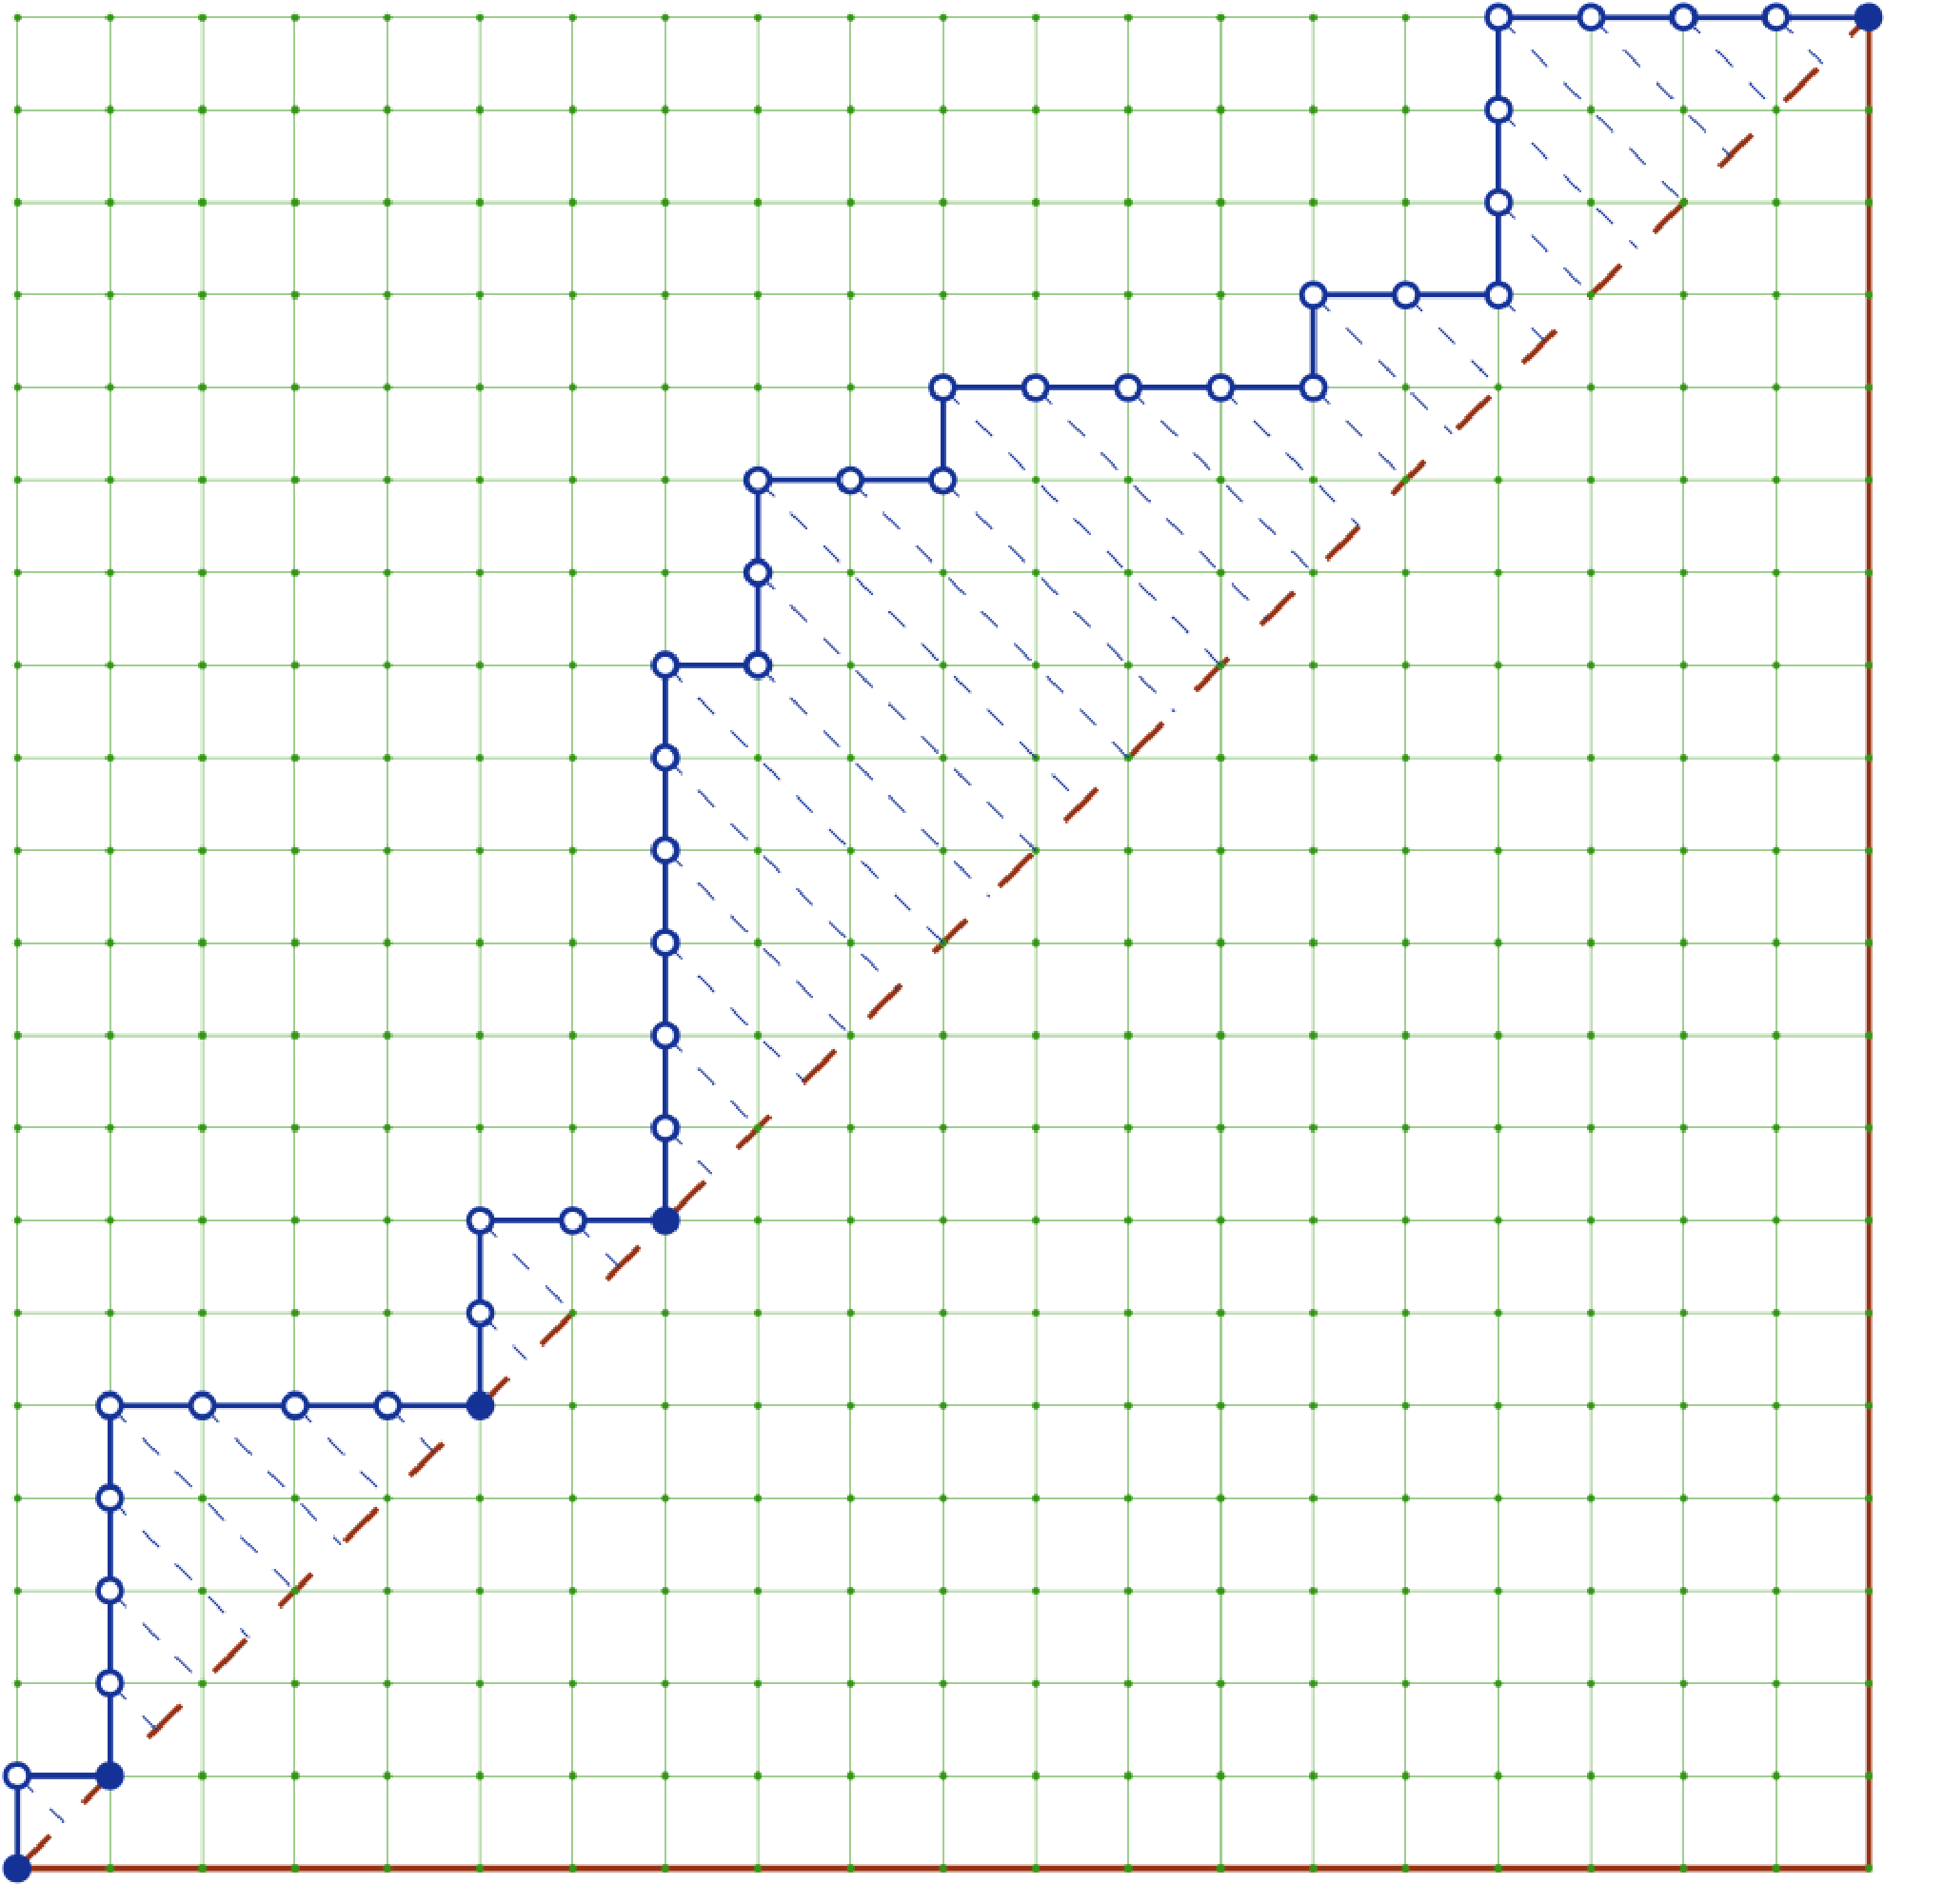
\includegraphics[width=0.7\textwidth]{dyck/basic_dyck_path.pdf}
    \caption{Simple Dyck path from $(0, 0)$ to $(20, 20)$}
    \label{fig:basic_dyck}
\end{figure}


\subsection{Catalan Trapezoids and Generalized Dyck Paths}
First, we define Catalan trapezoids as presented in \cite{trap}.
Let $C_k(n,m)$ be the $(n,m)^{th}$ entry of the Catalan trapezoid of order $k$, where $C_1(n,m)$ corresponds to the Catalan triangle.

The interpretation is as follows:
Consider a random walk from $(0,0)$ to $(m, n)$ ($n$ steps along the $y$-axis, and $m$ steps along the $x$-axis),
such that for any position $(x, y)$ along the walk, $y-x > 1-k$ (Figure~\ref{fig:complex_dyck})
i.e. the walk is always on one side of the shifted diagonal.
The total number of such paths is exactly $C_k(n,m)$.
For $k = 1$, we obtain the definition of the simple Dyck path (Figure~\ref{fig:basic_dyck}).

Now, we state a result from \cite{trap} without proof
$$
C_k(n,m)=
\begin{cases}
{n+m}\choose m &0\le m<k\\
{{n+m}\choose{m}} - {{n+m}\choose{m-k}} &k\le m\le n+k-1\\
0 &m>n+k-1
\end{cases}
$$

\begin{figure}[htbp]
    \centering
    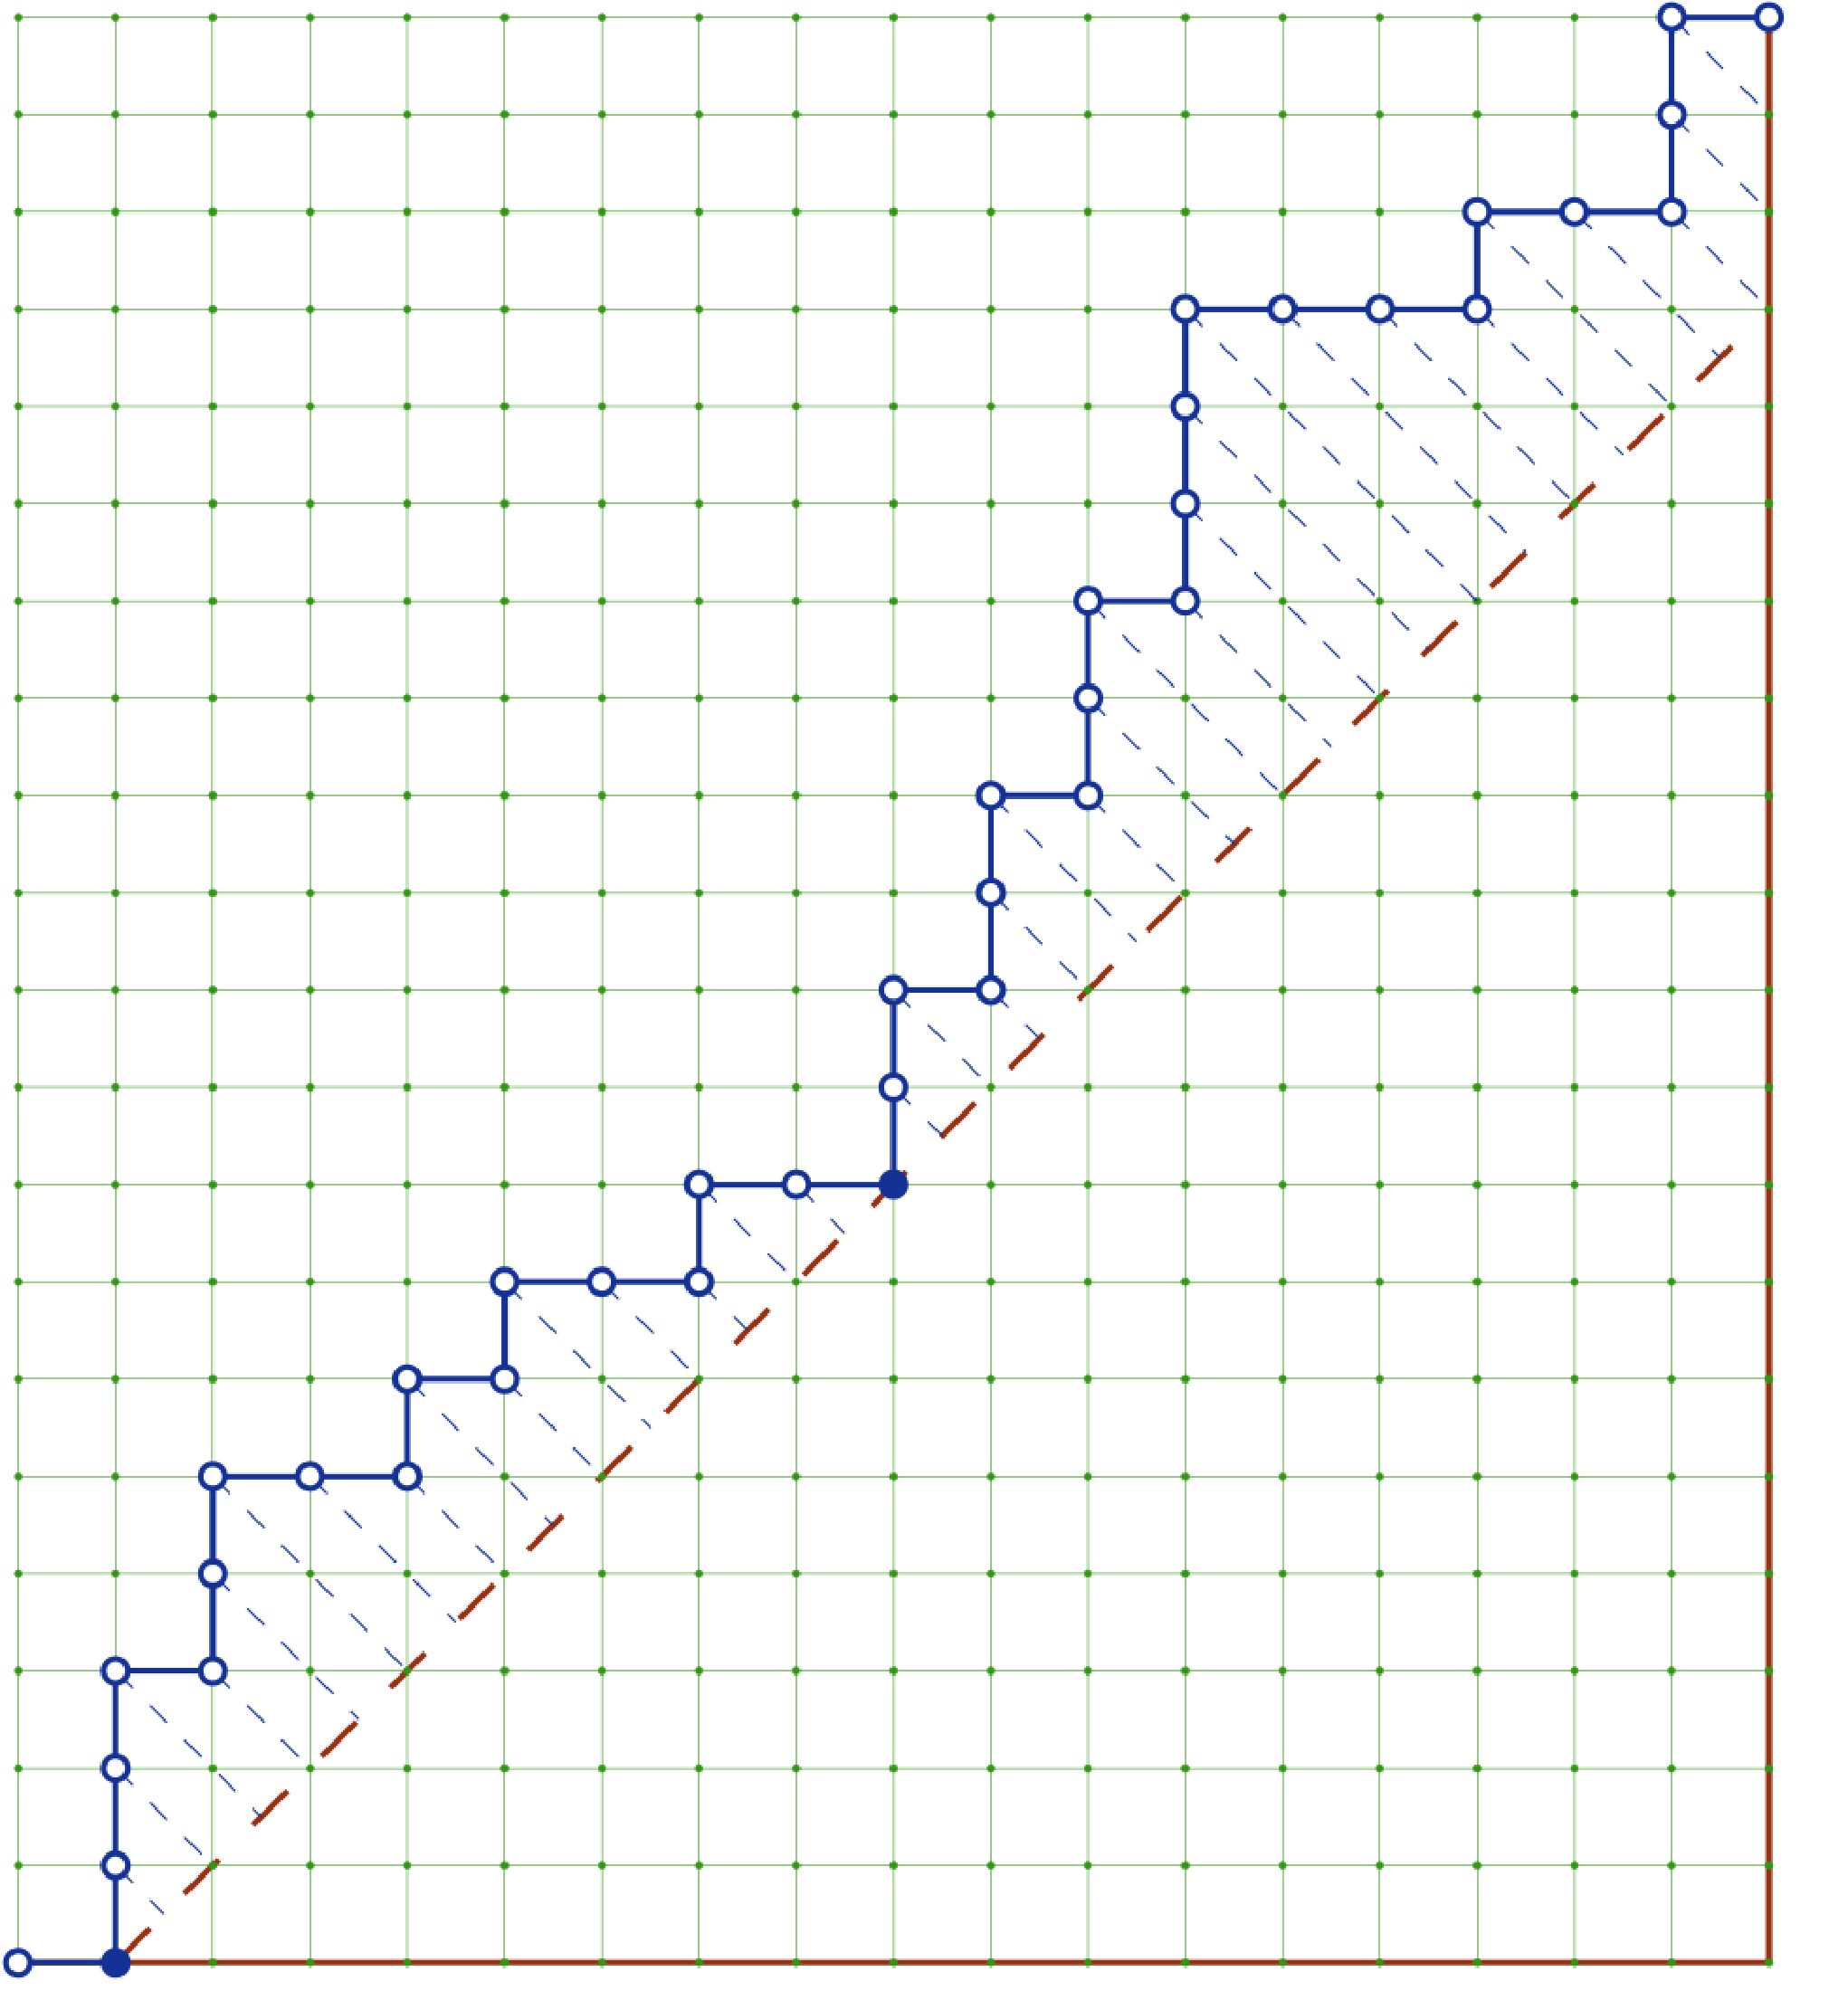
\includegraphics[width=0.7\textwidth]{dyck/complex_dyck_path.pdf}
    \caption{Complex Dyck path from $(0, 0)$ to $(18, 20)$ with $k = 2$. Notice that the diagonal is shifted.}
    \label{fig:complex_dyck}
\end{figure}

\subsection{Generating Dyck Paths}
Our general recursive step is as follows.
We consider a sequence of length $2S$ comprising of $2U$ up moves ($+1$) and $2D$ down moves ($-1$).
Additionally, the sum of any initial sequence {\color{red} prefix?} canon be less than $k-1$.
Without loss of generality, let's assume that $2D\le S$. If this were not the case,
we could simply flip the sequence and negate the elements.
This essentially means that the overall Dyck path is non-decreasing.

\begin{lemma}
$S-2D = \Bo(\log n\sqrt S) \implies U-D = \Bo(\log n\sqrt S)$
\label{lem:dyck_var0}
\end{lemma}

We want to sample the height of this path after $S$ steps.
This is the same as sampling the number of $(+1)$s that get assigned to the first half of the elements in the sequence.
We define $p_d$ as the probability that exactly $D-d$ $(-1)$s get assigned to the first half.
This means that exactly $U+d$ $(+1)$s get assigned to the first half.
Consequently, the second half will contain exactly $D+d$ $(-1)$s and $U-d$ $(+1)$s.

Let us first compute this probability.
$$
p_d = \frac{D_{left}\cdot D_{right}}{D_{tot}}
$$
Where $D_{left}$ denotes the number of valid starting sequences (first half)
and $D_{right}$ denotes the number of valid ending sequences.
Here, \textit{valid} means that each half sequence gets the appropriate number of ups and downs
and the initial sums never drop below $1-k$.
For, $D_{right}$, we will start the Dyck path from the end of the $2S$ sequence.
In this case the invalidation threshold will be a different $k'$.
This $k'$ is the final height of the $2S$ sequence. So, $k'=k+2U-2D = k+4S-2D$. We will use this fact extensively moving forward.

Also, $D_{tot}$ is the total number of possible sequences of length $2S$ , given the initial conditions.
This value is considered by constructing paths in the original direction i.e. the value of $k$ is the same.

\subsection{The Simple Case}
The problem of sampling reduces to the binomial sampling case when $k > \mathcal{O}(\log n)\sqrt S$ for some constant $c$.
In this case, the we can simply approximate the probability as
$$
\frac{{{S}\choose{D-d}}\cdot{{S}\choose{D+d}}}{{{2S}\choose{2D}}}
$$
This is because the random paths will not have initial sums less than $1-k$ with high probability.
Note that this uses the assumption that we have an increasing path.

\subsection{Path Segments Close to Zero}
The problem arises when we $k <\mathcal{O}(\log n)\sqrt{S}$. In this case we need to compute the actual probability,
Using the formula from \cite{trap}, we find that.
\begin{align}
D_{left} = {{S}\choose{D-d}}-{{S}\choose{D-d-k}} &&D_{right} = {{S}\choose{U-d}}-{{S}\choose{U-d-k'}}
\end{align}
Here, $k' = k+2U-2D$, and so $k' = \Bo(\log n)\sqrt S$.\todo{prove using Lemma~\ref{lem:dyck_var0}}

Finally, we compute the total number of Dyck paths as
$$
D_{tot} = {{2S}\choose{2D}}-{{2S}\choose{2D-k}}
$$

Now, we are going to use the following Lemma from \cite{huge}.
\begin{lemma}
\label{lem:huge}
Let $\{p_i\}$ and $\{q_i\}$ be distributions satisfying the following conditions
\begin{enumerate}
    \item There is a poly-time algorithm to approximate $p_i$ and $q_i$ up to $\pm n^{-2}$
    \item Generating an index $i$ according to $q_i$ is closely implementable.
    \item There exists a $poly(log n)$-time recognizable set $S$ such that
    \begin{itemize}
        \item $1-\SL{i\in S}{} p_i$ is negligible
        \item There exists a constant $c$ such that for every $i$, it holds that $p_i\le \log^{\mathcal{O}(1)} n\cdot q_i$
    \end{itemize}
\end{enumerate}
Then, generating an index $i$ according to the distribution $\{p_i\}$ is closely-implementable.
\end{lemma}

In this process, we will first disregard all values of $d$ where $|d|>\Theta(\sqrt S)$.
The probability mass associated with these values can be shown to be negligible \todo{bound variance of path}.

Next, we will construct an appropriate $\{q_i\}$ and show that $p_d < \log^{\mathcal{O}(1)} n\cdot q_d$
for all $|d|<\Theta(\sqrt S)$ and some constant $c$.
We will use the following distribution
$$
q_d = \frac{{S\choose D-d}\cdot{S\choose D+d}}{{2S\choose 2D}} = \frac{{S\choose D-d}\cdot{S\choose U-d}}{{2S\choose 2D}}
$$
It is shown in \cite{huge} that this distribution is closely implementable.

\begin{lemma}
First we show that $D_{left} \le \frac{c_1\cdot k}{\sqrt{S}}\cdot{{S}\choose{D-d}}$ for some constant $c_1$.
\end{lemma}
\begin{proof}
This involves some simple manipulations.
\begin{align}
D_{left} &= {{S}\choose{D-d}}-{{S}\choose{D-d-k}}\\
&= {{S}\choose{D-d}}\cdot \left[1-\frac{(D-d)(D-d-1)\cdots(D-d-k+1)}{(S-D-d+k)(S-D-d+k-1)\cdots(S-D-d+1)}\right]\\
&\le {{S}\choose{D-d}}\cdot \left[1-\left(\frac{D-d-k+1}{S-D+d+k}\right)^k\right]\\
&\le {{S}\choose{D-d}}\cdot \left[1-\left(\frac{U+d+k-(U-D+d+k-1)}{U+d+k}\right)^k\right]\\
&\le {{S}\choose{D-d}}\cdot \left[1-\left(\frac{U+d+k-\Bo(\sqrt{U})}{U+d+k}\right)^k\right]\\
&\le \frac{k}{\Theta(\sqrt{S})}\cdot{{S}\choose{D-d}}
\end{align}
\end{proof}

\begin{lemma}
Similarly, we show that $D_{right} < \frac{c_2\cdot k'}{\sqrt{S}}\cdot{{S}\choose{U-d}}$ for some constant $c_2$.
\end{lemma}
\begin{proof}
\begin{align}
D_{right} &= {{S}\choose{U-d}}-{{S}\choose{U-d-k'}}\\
&= {{S}\choose{U-d}}\cdot \left[1-\frac{(U-d)(U-d-1)\cdots(U-d-k'+1)}{(S-U-d+k')(S-U-d+k'-1)\cdots(S-U-d+1)}\right]\\
&\le {{S}\choose{U-d}}\cdot \left[1-\left(\frac{U-d-k'+1}{S-U+d+k'}\right)^{k'}\right]\\
&\le {{S}\choose{U-d}}\cdot \left[1-\left(\frac{2D-U-d-k+1}{2U-D+k+d}\right)^{k'}\right]\\
&\le {{S}\choose{U-d}}\cdot \left[1-\left(\frac{U+k+d - (2U-2D+2d+2k-1)}{U+k+d}\right)^{k'}\right]\\
&\le {{S}\choose{U-d}}\cdot \left[1-\left(\frac{U+k+d - \Bo(\sqrt U)}{U+k+d}\right)^{k'}\right]\\
&\le \frac{k'}{\Theta(\sqrt{S})}\cdot{{S}\choose{U-d}}
\end{align}
\end{proof}

Finally, we need to lower bound the value of $D_{tot}$.

\begin{lemma}
We claim that $D_{tot} < \frac{c_3\cdot k\cdot k'}{S}\cdot{{2S}\choose{2D}}$ for some constant $c_3$.
\end{lemma}
\begin{proof}
\begin{align}
D_{tot} &= {{2S}\choose{2D}}-{{2S}\choose{2D-k}}\\
&= {{2S}\choose{2D}}\cdot \left[1-\frac{(2D)(2D-1)\cdots(2D-k+1)}{(2S-2D+k)(2S-2D+k-1)\cdots(2S-2D+1)}\right]\\
&\ge {{2S}\choose{2D}}\cdot \left[1-\left(\frac{2D-k+1}{2S-2D+1}\right)^k\right]\\
&\ge {{2S}\choose{2D}}\cdot \left[1-\left(\frac{2U-(2U-2D+k-1)}{2U+1}\right)^k\right]\\
&\ge {{2S}\choose{2D}}\cdot \left[1-\left(\frac{(2U+1)-k'}{2U+1}\right)^k\right]\\
&\ge \frac{k\cdot k'}{\Theta(S)}\cdot{{2S}\choose{2D}}
\end{align}
\end{proof}

\begin{theorem}
We can now put these lemmas together to show that $p_d/q_d \le c = c_1\cdot c_2/c_3 = \Theta(1)$.
This satisfies all the conditions of Lemma~\ref{lem:huge} from \cite{huge}.
We simply need to set the accept probability less than $p_d/(c\cdot q_d)$.
\end{theorem}


%\section{Domino Tiling the $2\times n$ grid}
We will consider the problem of tiling a square grid with dominos.
This problem has a long history and various importtant applications in statistical physics.
Specifically, we will focus on the local generation of domino tilings of a $2\times n$ grid from the uniform distribution.
The queries will be as an index, and the generator should report the orientation of the domino at the $i^{th}$ position in the grid.
%\begin{figure}[htbp]
    %\centering
    %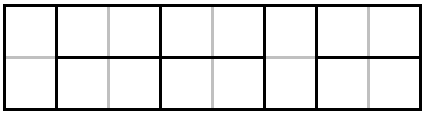
\includegraphics[width=\textwidth]{images/domino2.png}
    %\caption{}
    %\label{fig:dom2}
%\end{figure}

It is a well known result \todo{cite} that the number of tilings of a $2\times n$ grid is exactly $F_n$.
To aid with generalization, we will instead allow the generator to respond with the splitting boundary of the current tiling instead.
For example, in Figure~\ref{fig:b20}, the boundary is a vertical line at the specified position.
In Figure~\ref{fig:b21}, the boundary is horizontal, indicating that there are two horizontal dominos at that location.
Note that Figure~\ref{fig:b22} is impossible for a $2\times n$ grid.
It should be clear that this query model is equivalent.

\begin{figure}[h]
    \centering
    \begin{subfigure}[b]{0.4\textwidth}
        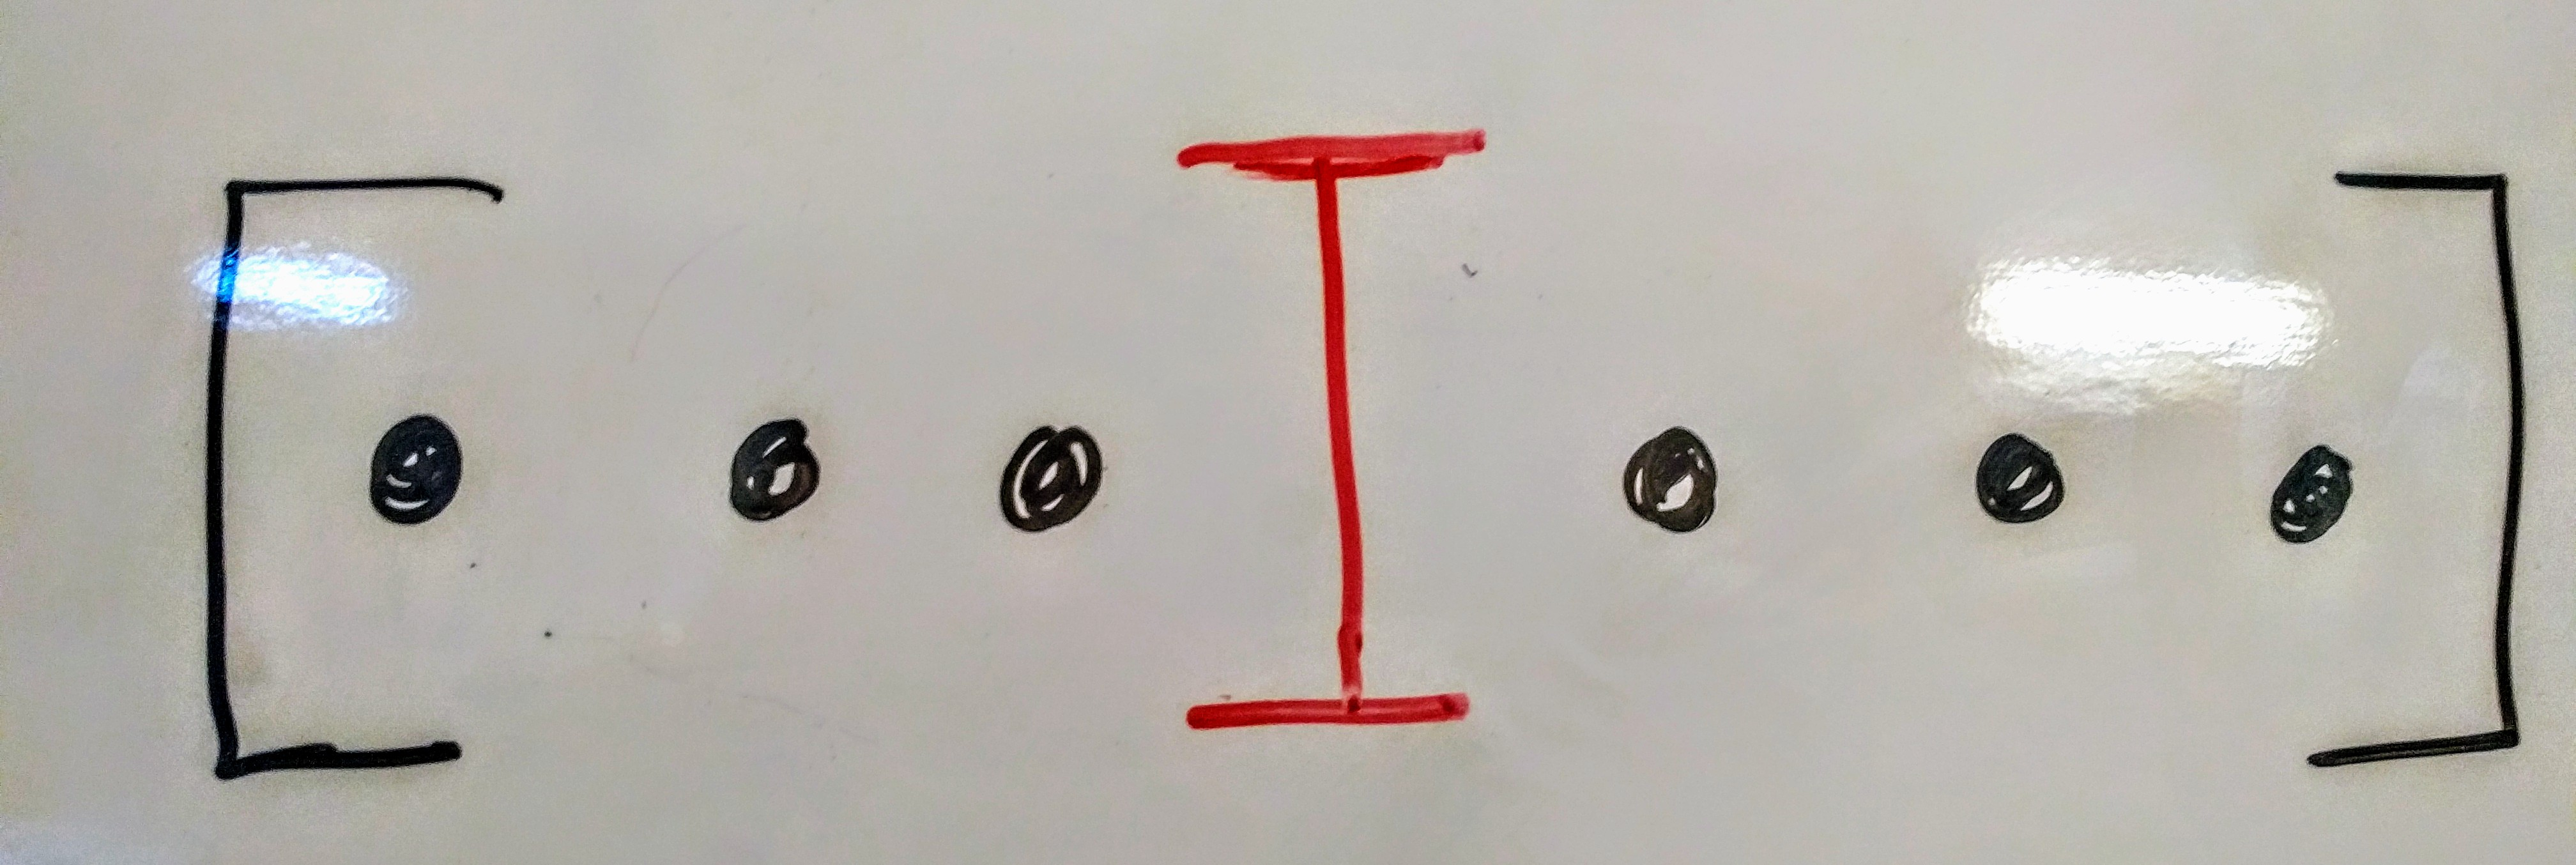
\includegraphics[width=\linewidth]{images/tile2-0.jpg}
        \label{fig:b20}
    \end{subfigure}
    \begin{subfigure}[b]{0.4\textwidth}
        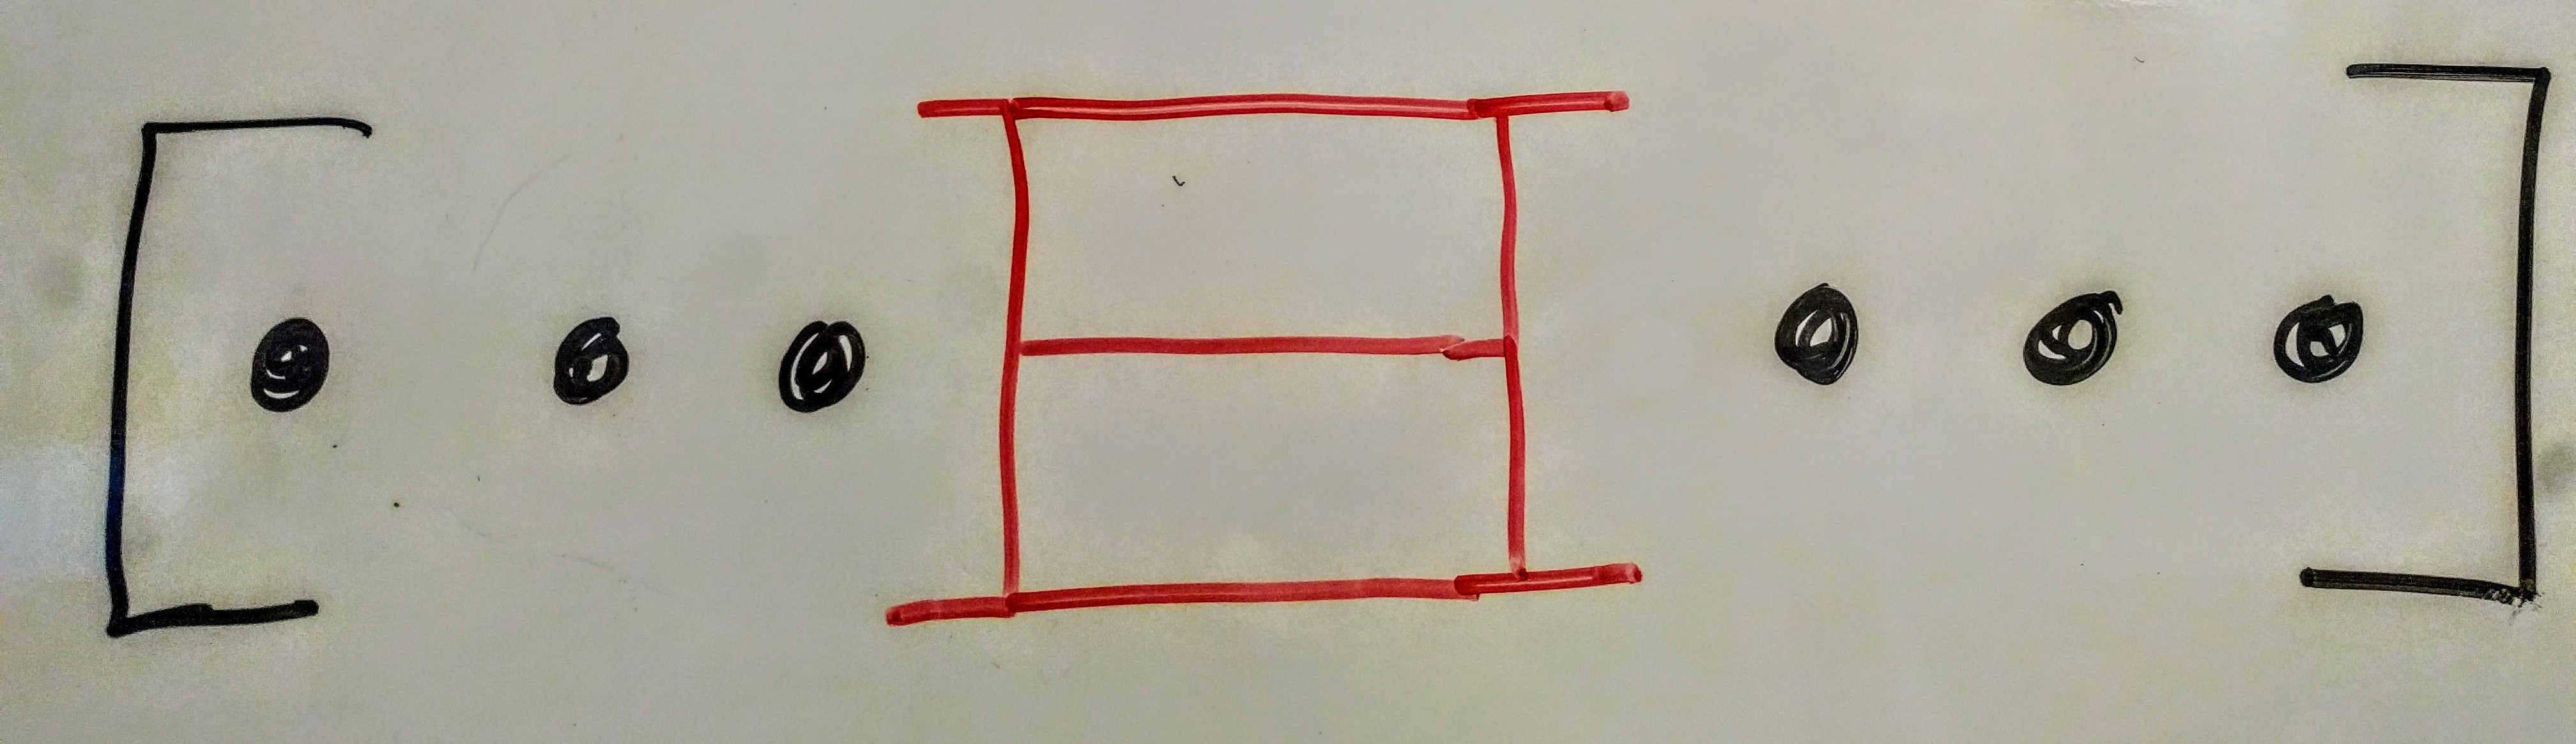
\includegraphics[width=\linewidth]{images/tile2-1.jpg}
        \label{fig:b21}
    \end{subfigure}

    \begin{subfigure}[b]{0.5\textwidth}
        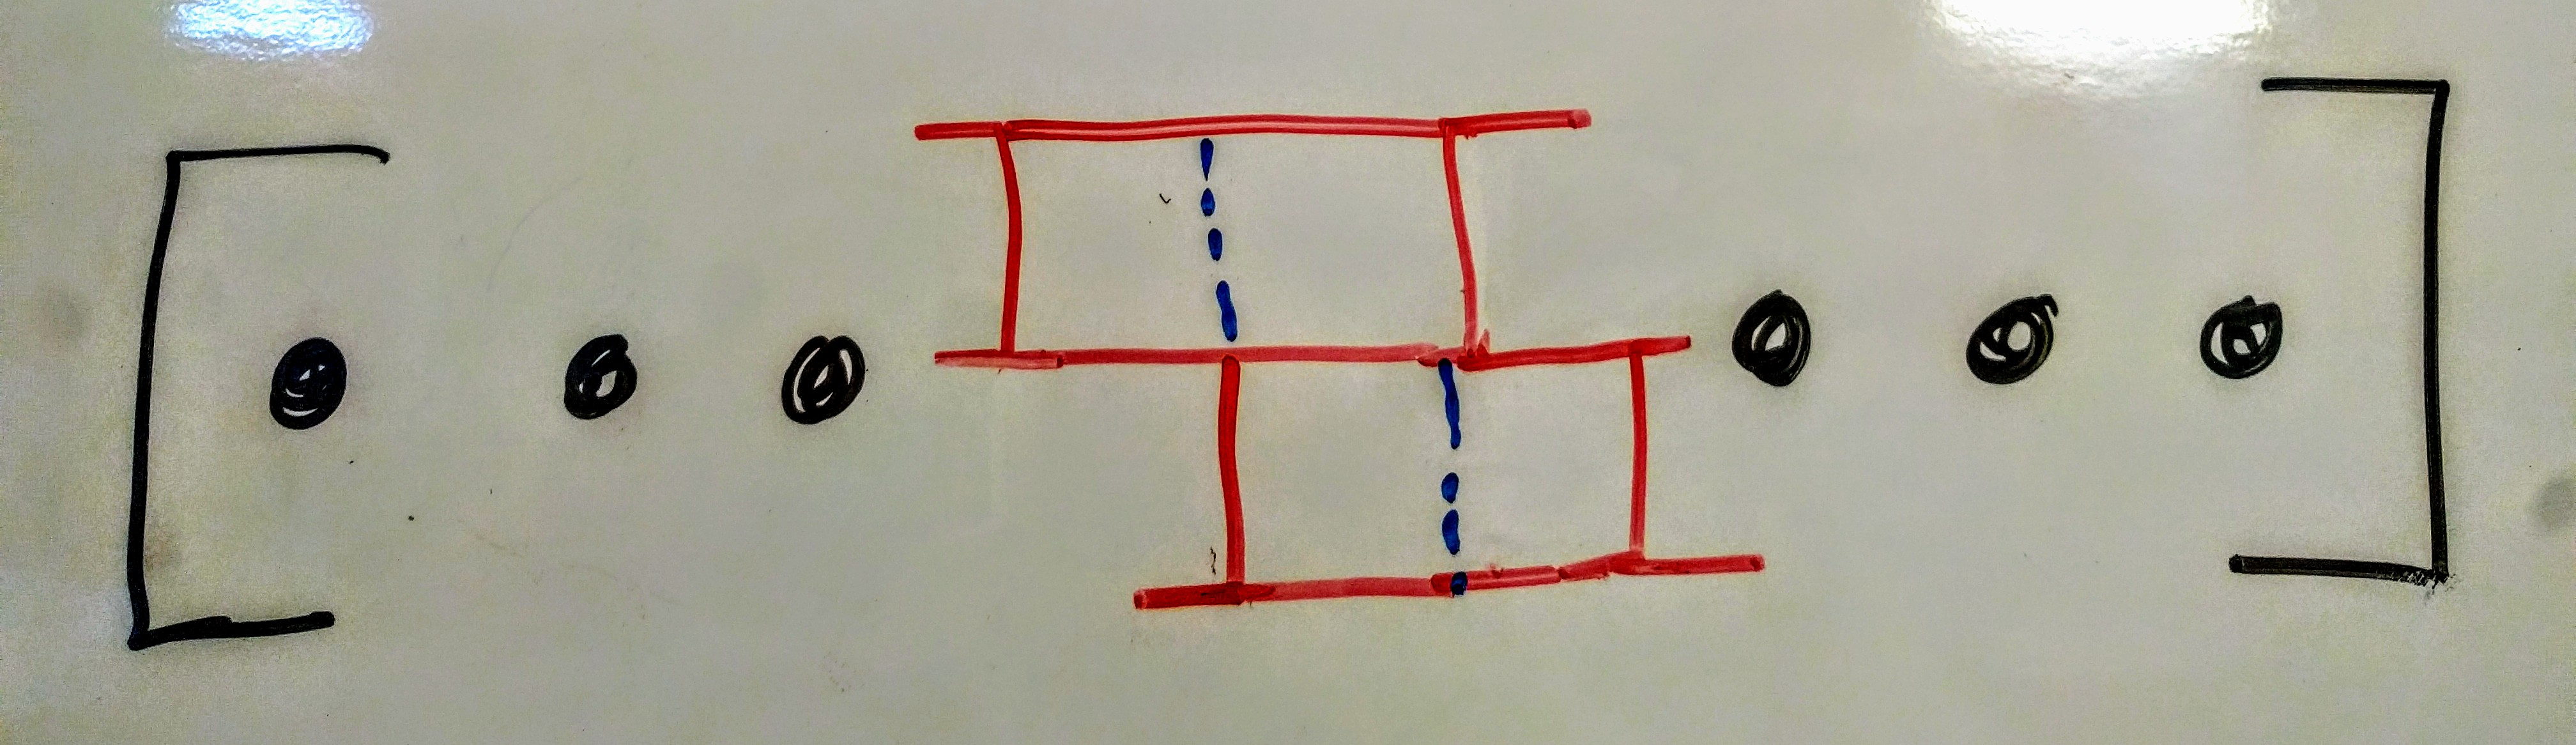
\includegraphics[width=\linewidth]{images/tile2-2.jpg}
        \label{fig:b22}
    \end{subfigure}
    \caption{Caption for this figure with two images}
    \label{fig:boundary2}
\end{figure}

Now, consider a query to the location $i$, such that all positions between $i-a$ and $i+b$ have not been queriesd so far.
So, there is a blank $2\times(a+b)$ size sub-grid that we have to sample from.
Let us consider the number of possible tilings resulting from each possible splitting boundary.
\begin{enumerate}
    \item Vertical Boundary -- This indicates that we divide the region into two sub-grids with sizes
          $2\times a$ and $2\times b$.
          So, the total number of possible tilings is exactly $F_a\cdot F_b$.
    \item Horizontal Boundary -- This indicates that we divide the region into two sub-grids with sizes
          $2\times (a-1)$ and $2\times (b-1)$.
          So, the total number of possible tilings is exactly $F_{a-1}\cdot F_{b-1}$.
\end{enumerate}

So the probabilities are computed as $\frac{F_a\cdot F_b}{F_a\cdot F_b + F_{a-1}\cdot F_{b-1}}$
and $\frac{F_{a-1}\cdot F_{b-1}}{F_a\cdot F_b + F_{a-1}\cdot F_{b-1}}$.
Now, we face the issue of approximating these fractions.
If either of the values $a$ or $b$ are less than $\Theta(\sqrt n)$,
then we can compute the exact value of the corresponding $F_a$ or $F_b$.
Otherwise, we use Lemma~\ref{lem:rat_conv} to approximate $F_a=\phi\cdot F_{a-1}$ and $F_b=\phi\cdot F_{b-1}$.
So, the probability of the vertical boundary becomes
$$
\frac{F_a\cdot F_b}{F_a\cdot F_b + F_{a-1}\cdot F_{b-1}} = \frac{\phi^2}{\phi^2+1}
$$
Similarly, the probability of a horizontal split with a top and bottom domino becomes $1/(\phi^2+1)$.
Note that this also determines the two adjacent boundaries.

The only information we needed to make this query was the extent of the un-queried interval $[i-a, i+b]$.
We can use any standard data-structure that allows insertion in positions $\{1, 2\cdots,n+1\}$,
and provides successor and predecessor queries.

Here's we can be fancy and use Van-Emde-Boas trees to get a $\Bo(\log\log n)$ query time.
However, in some cases, the exact value of a Fibonacci number still needs to be computed, and this takes $\Bo(\log n)$ time.
The faster queries only work when the new query is "far enough" ($\Bo(\log n)$ distance) away from all previous queries.


%\subsection{Permutations}

\anak{Did we try to support more information that just computing $\pi(i)$?}
[Specification]

In addition to a table (dictionary) containing all assigned values $\pi(i)$, we maintain the following binary trees,
whose nodes are generated on-the-fly in response to queries.

$T_1$: Each node of $T_1$ corresponds to a specific range of indices,
where the root represents the entire range $\{1, \ldots, N\}$,
and its two children represents each (approximately) half of the parent's range.
Each node counts the indices $i$ in the range, such that $\pi(i) = \bot$.
Initially $T_1$ only contains the root node, and the number of unassigned indices are $N$.
The children are only generated when we need to traverse down from the root; as these nodes are generated,
all of the indices in their ranges are unassigned.
Once an index becomes assigned, we simply update the information along the path in $\Bo(\log n)$ time.

$T_2$: $T_2$ is similar to $T_1$ but instead of maintaining the number of indices in the range that are still unassigned,
it maintains the number of values in the range that are still unused (have not been assigned to an index).
Similarly, we may sample an unused value or mark it as used within $\Bo(\log n)$ time.

To compute $\pi(i)$, first we check the table for $\pi(i)$ and return its value if $\pi(i)\neq\bot$.
Otherwise, sample an unused value $j$ from $T_2$ and mark that value as used.
Add $\pi(i) = j$ to the table, and mark index $i$ as used on $T_1$.

If we wish to support $\pi^{-1}(i)$, then also store the table of $\pi^{-1}(i)$.
To assign $\pi^{-1}(i)$, sample an unassigned index $j$ from $T_1$ then mark it as assigned,
add $\pi(j)=i$ and $\pi^{-1}(i)=j$ to the table, and mark the value $i$ as used on $T_2$.

\subsection{Generating Permutations with given Cyclic Structure}
We will use the technique from \cite{cyclic} to locally generate a random permutation with a given cyclic structure.
This algorithm uses two permutations $\pi$ and $\sigma$,
where $\pi$ is a uniformly random permutation and $\sigma$ is a fixed permutation with the given structure.
The resulting random permutation is formed by the composition $\pi^{-1}(\sigma(\pi(\cdot)))$.
We will generate the permutation $\pi$ as described in the previous section.;



We receive as input a list of cycle sizes \{$c_1, c_2,\cdots, c_k\}$ with the restriction that $\sum c_i = n$.
Now we need to locally generate the permutation $\sigma$ with the prescribed structure.
Define the indices $C_j = \SL{i=1}{j}c_i$ with $C_0 = 0$.
We will construct the cycle corresponding to $c_i$ as all the elements in the interval $\{c_{i-1}+1,c_{i-1}+2,\cdots,c_i\}$.

Of course we will not be computing $\sigma$ explicitly.
Instead, we will pre-compute the $C_j$ indices, and when given a query $\sigma(x)$,
we binary search amongst $C_j$ to find the cycle that $x$ belongs to.
Then we can report the value of $\sigma(x)$ accordingly.

So, we can now compose the generator oracles for $\pi$, $\sigma$, and $\pi^{-1}$ to get the full generator. 

%\section{Random Coloring of a Graph}%
\label{sec:random_coloring_of_a_graph}

We wish to locally sample an uniformly random coloring of a graph.
A $q$-coloring of a graph $G = (V, E)$ is a function $\sigma : V\rightarrow [q]$,
such that for all $(u,v)\in E$, $\sigma_u \not= \sigma_v$.
We will consider only bounded degree graphs, i.e. graphs with max degree $\le \Delta$.
Otherwise, the coloring problem becomes NP-hard\todo{cite}.

Using the technique of path-coupling, Vigoda \todo{cite} showed that for $q > 2\Delta$,
one can sample an uniformly random coloring by using a MCMC algorithm.

\subsection{Glauber Dynamics}%
\label{sub:glauber_dynamics}

The Markov Chain proceeds in $T$ steps. The state of the chain at time $t$ is given by $\vec X^t\in [q]^{|V|}$.
Specifically, the color of vertex $v$ at step $t$ is $\vec X^t_v$.

In each step of the Markov process, a pair $(v, c)\in V\times [q]$ is sampled uniformly at random.
Subsequently, if the recoloring of vertex $v$ with color $c$ does not result in a conflict with $v$'s neighbors,
i.e. $c\not\in \left\{ X^t_u : u\in \Gamma(v)\right\}$, then the vertex is recolored i.e. $X_v^{t+1}\leftarrow c$.

After running the MC for $T = \mathcal{O}(n\log n)$ steps we reach the stationary distribution ($\epsilon$ close),
and the coloring is an uniformly random one.

\subsection{Local Coloring Algortihm}%
\label{sub:local_coloring_algortihm}

Given a vertex $v$, the local-access generator has to output the color of $v$
after running $T = \mathcal{O}(n\log n) = k\cdot n\log n$ steps of Glauber Dynamics where $k$ is a constant.
For this algorithm to work, we will take $q > 2k\Delta\log n = \mathcal{O}(\Delta\log n)$.

We can consider T iterations of the above MC, and the corresponding vertex and color samples.
\[
\left\langle (v_1, c_1), (v_2, c_2), (v_3, c_3), \cdots, (v_T, c_T)\right\rangle \thicksim_{\mathcal U} \left( V\times [q]\right)^T
\]
A position $i$ in the sequence is labeled \emph{``ACCEPT''} if at the $i^{th}$ step,
$v_i$ was recolored to $c_i$ (no conflicts with neighbors).
Otherwise, position $i$ is marked \emph{``REJECT''}.

Given a vertex $v$, we consider all instances of $(v, *)$, where $*\in [q]$.
Let the last such occurrence be $(v, c_t)$.
We now need to compute whether position $i$ was marked \emph{``ACCEPT''} or \emph{``REJECT''}.

\subsection{Modified Glauber Dynamics}%
\label{sub:modified_glauber_dynamics}

Now we define a modified Markov Chain, with each step called an epoch.
In the $i^{th}$ epoch, denoted by $\mathcal E_i$,
\begin{itemize}
    \item Pick a random permutation $\pi^{(i)}$ of the vertices $V$.
    \item Sample $n = |V|$ colors $ \langle c_1, c_2,\cdots, c_n \rangle$ from $[q]$.
    \item Perform the standard update using the pairs
          $\left\langle (\pi^{(i)}_1, c_1), (\pi^{(i)}_2, c_2), \cdots, (\pi^{(i)}_n, c_n)\right\rangle$.
\end{itemize}

\begin{theorem}
\label{thm:modified_mixing}
After $k\log n$ epochs, the Markov Chain is mixed.
\end{theorem}




\bibliographystyle{alpha}

\bibliography{bib}

\clearpage
\appendix
\label{sec:appendix}

\section{Further Analysis and Extensions of Algorithm~\ref{alg:oblivious-coin-toss}}
\label{sec:reroll-cont}

\subsection{Performance Guarantee}
This section is devoted to showing the following lemma that bounds the required resources per query of Algorithm~\ref{alg:oblivious-coin-toss}. We note that we only require efficient computation of $\prod_{u \in [a,b]} (1-p_{v,u})$ (and not $\sum_{u \in [a,b]} p_{v,u}$), and that for the $G(n,p)$ model, the resources required for such computation is asymptotically negligible.

\begin{restatable}{theorem}{res:ER-rand-iterations}\label{thm:ER-rand-iterations}
Each execution of Algorithm~\ref{alg:oblivious-coin-toss} (the \func{next-neighbor} query), with high probability,
\begin{itemize}
\item terminates within $\bo(\log n)$ iterations (of its \textup{\textbf{repeat}} loop);
\item computes $\bo(\log^2 n)$ quantities of $\prod_{u \in [a,b]} (1-p_{v,u})$;
\item aside from the above computations, uses $\bo(\log^2 n)$ time, $\bo(\log n)$ random $N$-bit words, and $\bo(\log n)$ additional space.
\end{itemize}
\end{restatable}

\begin{proof}
We focus on the number of iterations as the remaining results follow trivially. This proof is rather involved and thus is divided into several steps.

\paragraph{Specifying random choices} The performance of the algorithm depends on not only the random variables $X_{v,u}$'s, but also the unused coins $C_{v,u}$'s. We characterize the two collections of Bernoulli variables $\{X_{v,u}\}$ and $\{Y_{v,u}\}$ that cover all random choices made by Algorithm~\ref{alg:oblivious-coin-toss} as follows.

\begin{itemize}
\item Each $X_{v,u}$ (same as $X_{u,v}$) represents the result for the \emph{first} coin-toss corresponding to cells $\ADJ[v][u]$ and $\ADJ[u][v]$, which is the coin-toss obtained when $X_{v,u}$ becomes decided: either $C_{v,u}$ during a \func{next-neighbor}$(v)$ call when $\ADJ[v][u] = \PHI$, or $C_{v,u}$ during a \func{next-neighbor}$(u)$ call when $\ADJ[u][v] = \PHI$, whichever occurs first.
This description of $X_{v,u}$ respects our invariant that, if the generation process is executed to completion, we will have $\ADJ[v][u]=X_{v,u}$ in all entries.
\item Each $Y_{v,u}$ represents the result for the \emph{second} coin-toss corresponding to cell $\ADJ[v][u]$, which is the coin-toss $C_{v,u}$ obtained during a \func{next-neighbor}$(v)$ call when $X_{v,u}$ is already decided. In other words, $\{Y_{v,u}\}$'s are the coin-tosses that should have been skipped but still performed in Algorithm~\ref{alg:oblivious-coin-toss} (if they have indeed been generated). Unlike the previous case, $Y_{v,u}$ and $Y_{u,v}$ are two independent random variables: they may be generated during a \func{next-neighbor}$(v)$ call and a \func{next-neighbor}$(u)$ call, respectively.
\end{itemize}
As mentioned earlier, we allow any sequence of probabilities $p_{v,u}$ in our proof. The success probabilities of these indicators are therefore given by $\pp[X_{v,u}=\ONE] = \pp[Y_{v,u}=\ONE] = p_{v,u}$.

%\anak{Consider improving paragraph below.}
\paragraph{Characterizing iterations}
Suppose that we compute \func{next-neighbor}$(v)$ and obtain an answer $u$. Then $X_{v,\LAST[v]+1} = \cdots = X_{v, u-1} = \ZERO$ as none of $u' \in (\LAST[v], u)$ is a neighbor of $v$. The vertices considered in the loop of Algorithm~\ref{alg:oblivious-coin-toss} that do not result in the answer $u$, are $u' \in (\LAST[v], u)$ satisfying $\ADJ[v][u'] = \ZERO$ and $Y_{v,u'} = \ONE$; we call the iteration corresponding to such a $u'$ a \emph{failed iteration}. Observe that if $X_{v,u'} = \ZERO$ but is undecided ($\ADJ[v][u'] = \PHI$), then the iteration is not failed, even if $Y_{v,u'} = \ONE$ (in which case, $X_{v,u'}$ takes the value of $C_{v,u'}$ while $Y_{v,u'}$ is never used). Thus we assume the worst-case scenario where all $X_{v,u'}$ are revealed: $\ADJ[v][u']=X_{v,u'}=\ZERO$ for all $u'\in(\LAST[v], u)$. The number of failed iterations in this case stochastically dominates those in all other cases.\footnote{There exists an adversary who can enforce this worst case. Namely, an adversary that first makes \func{next-neighbor} queries to learn all neighbors of every vertex except for $v$, thereby filling out the whole $\ADJ$ in the process. The claimed worst case then occurs as this adversary now repeatedly makes \func{next-neighbor} queries on $v$. In particular, a committee of $n$ adversaries, each of which is tasked to perform this series of calls corresponding to each $v$, can always expose this worst case.}

Then, the upper bound on the number of failed iterations of a call \func{next-neighbor}$(v)$ is given by the maximum number of cells $Y_{v, u'} = 1$ of $u' \in(\LAST[v], u)$, over any $u \in(\LAST[v], n]$ satisfying $X_{v,\LAST[v]+1} = \cdots = X_{v,u} = \ZERO$. Informally, we are asking ''of all consecutive cells of $\ZERO$'s in a single row of $\{X_{v,u}\}$-table, what is the largest number of cells of $\ONE$'s in the corresponding cells of $\{Y_{v,u}\}$-table?''

\paragraph{Bounding the number of iterations required for a fixed pair $(v, \LAST[v])$}
We now proceed to bounding the number of iterations required over a sampled pair of $\{X_{v,u}\}$ and $\{Y_{v,u}\}$, from any probability distribution. For simplicity we renumber our indices and drop the index $(v,\LAST[v])$ as follows. Let $p_1, \ldots, p_L \in [0, 1]$ denote the probabilities corresponding to the cells $\ADJ[v][\LAST[v]+1 \ldots n]$ (where $L = n-\LAST[v]$), then let $X_1, \ldots, X_L$ and $Y_1, \ldots, Y_L$ be the random variables corresponding to the same cells on $\ADJ$.

For $i=1, \ldots, L$, define the random variable $Z_i$ in terms of $X_i$ and $Y_i$ so that
\begin{itemize}
\item $Z_i = 2$ if $X_i = 0$ and $Y_i = 1$, which occurs with probability $p_i(1-p_i)$. \\
This represents the event where $i$ is not a neighbor, and the iteration fails.
\item $Z_i = 1$ if $X_i = Y_i = 0$, which occurs with probability $(1-p_i)^2$.\\
 This represents the event where $i$ is not a neighbor, and the iteration does not fail.
\item $Z_i = 0$ if $X_i = 1$, which occurs with probability $p_i$. \\
This represents the event where $i$ is a neighbor.
\end{itemize}

For $\ell \in [L]$, define the random variable $M_\ell := \prod_{i=1}^\ell Z_i$, and $M_0 = 1$ for convenience. If $X_i = 1$ for some $i \in [1, \ell]$, then $Z_i = 0$ and $M_\ell = 0$. Otherwise, $\log M_\ell$ counts the number of indices $i \in [\ell]$ with $Y_i = 1$, the number of failed iterations. Therefore, $\log(\max_{\ell \in \{0, \ldots, L\}} M_\ell)$ gives the number of failed iterations this \func{next-neighbor}$(v)$ call.

To bound $M_\ell$, observe that for any $\ell\in[L]$, $\mathbb{E}[Z_\ell] = 2p_\ell(1-p_\ell) + (1-p_\ell)^2 = 1 - p_\ell^2 \leq 1$ regardless of the probability $p_\ell \in [0, 1]$. Then, $\mathbb{E}[M_\ell] = \mathbb{E}[\prod_{i=1}^\ell Z_i] = \prod_{i=1}^\ell \mathbb{E}[Z_i] \leq 1$ because $Z_\ell$'s are all independent. By Markov's inequality, for any (integer) $r \geq 0$, $\Pr[\log M_\ell > r] = \Pr[M_\ell > 2^r] < 2^{-r}$. By the union bound, the probability that more than $r$ failed iterations are encountered is $\Pr[\log(\max_{\ell \in \{0, \ldots, L\}} M_\ell) > r] < L\cdot 2^{-r} \leq n\cdot 2^{-r}$.

\paragraph{Establishing the overall performance guarantee}
So far we have deduced that, for each pair of a vertex $v$ and its $\LAST[v]$, the probability that the call \func{next-neighbor}$(v)$ encounters more than $r$ failed iterations is less that $n \cdot 2^{-r}$, which is at most $n^{-c-2}$ for any desired constant $c$ by choosing a sufficiently large $r = \Theta(\log n)$. As Algorithm~\ref{alg:oblivious-coin-toss} may need to support up to $\Theta(n^2)$ \func{next-neighbor} calls, one corresponding to each pair $(v, \LAST[v])$, the probability that it ever encounters more than $O(\log n)$  failed iterations to answer a single \func{next-neighbor} query is at most $n^{-c}$. That is, with high probability, $O(\log n)$ iterations are required per \func{next-neighbor} call, which concludes the proof of Theorem~\ref{thm:ER-rand-iterations}.
%For the $G(n,p)$ model, each iteration requires $O(\log n)$ time and random bits (for sampling), so this bound on the number of iterations implies that each \func{next-neighbor} call requires $O(\log^2 n)$ time, $O(1)$ additional space for the maintained data structure, and $O(\log^2 n)$ random bits with high probability. The former two offer an improvement over Algorithm~\ref{alg:exact-coin-toss}, but note also that the bounds of Algorithm~\ref{alg:exact-coin-toss} holds deterministically.
\end{proof}

\subsection{Supporting \func{vertex-pair} Queries} \label{sec:ER-pair}

We extend our generator (Algorithm~\ref{alg:oblivious-coin-toss}) to support the \func{vertex-pair} queries: given a pair of vertices $(u, v)$, decide whether there exists an edge $\{u, v\}$ in the generated graph. To answer a \func{vertex-pair} query, we must first check whether the value $X_{u,v}$ for $\{u, v\}$ has already been assigned, in which case we answer accordingly. Otherwise, we must make a coin-flip with the corresponding bias $p_{u,v}$ to assign $X_{u,v}$, deciding whether $\{u, v\}$ exists in the generated graph. If we maintained the full $\ADJ$ as done in the na\"{i}ve Algorithm~\ref{alg:naive}, we would have been able to simply set $\ADJ[u][v]$ and $\ADJ[v][u]$ to this new value. However, our more efficient Algorithm~\ref{alg:oblivious-coin-toss} that represents $\ADJ$ compactly via $\LAST$ and $P_v$'s cannot record arbitrary modifications to $\ADJ$.

Observe that if we were to apply the trivial implementation of \func{vertex-pair} in Algorithm~\ref{alg:naive}, then by Lemma~\ref{lem:cond-0}, $\LAST$ and $P_v$'s will only fail capture the state $\ADJ[v][u] = \ZERO$ when $u > \LAST[v]$ and $v > \LAST[u]$. Fortunately, unlike \func{next-neighbor} queries, a \func{vertex-pair} query can only set one cell $\ADJ[v][u]$ to $\ZERO$ per query, and thus we may afford to store these changes explicitly.\footnote{The disadvantage of this approach is that the generator may allocate more than $\Theta(m)$ space over the entire graph generation process, if \func{vertex-pair} queries generate many of these $\ZERO$'s.} To this end, we define the set $Q = \{\{u,v\}: X_{u,v}\textrm{ is assigned to }\ZERO \textrm{ during a \func{vertex-pair} query}\}$, maintained as a hash table. Updating $Q$ during \func{vertex-pair} queries is trivial: we simply add $\{u,v\}$ to $Q$ before we finish processing the query if we set $\ADJ[u][v]=\ZERO$. Conversely, we need to add $u$ to $P_v$ and add $v$ to $P_u$ if the \func{vertex-pair} query sets $\ADJ[u][v]=\ONE$ as usual, yielding the following observation. It is straightforward to verify that each \func{vertex-pair} query requires $O(\log n)$ time, $O(1)$ random $N$-bit word, and $O(1)$ additional space per query.

\begin{restatable}{lem}{cond-q}\label{lem:cond-0-q}
The data structures $\LAST$, $P_v$'s and $Q$ together provide a succinct representation of $\ADJ$ when \func{next-neighbor} queries (modified Algorithm~\ref{alg:oblivious-coin-toss}) and \func{vertex-pair} queries (modified Algorithm~\ref{alg:naive}) are allowed. In particular, $\ADJ[v][u]=\ONE$ if and only if $u \in P_v$. Otherwise, $\ADJ[v][u]=\ZERO$ if $u <\LAST[v]$, $v < \LAST[u]$, or $\{v,u\} \in Q$. In all remaining cases, $\ADJ[v][u]=\PHI$.
\end{restatable}

We now explain other necessary changes to Algorithm~\ref{alg:oblivious-coin-toss}. In the implementation of \func{next-neighbor}, an iteration is not failed when the chosen $X_{v,u}$ is still undecided: $\ADJ[v][u]$ must still be $\phi$. Since $X_{v,u}$ may also be assigned to $\ZERO$ via a \func{vertex-pair}$(v,u)$ query, we must also consider an iteration where $\{v,u\} \in Q$ failed. That is, we now require one additional condition $\{v,u\} \notin Q$ for termination (which only takes $O(1)$ time to verify per iteration). As for the analysis, aside from handling the fact that $X_{v,u}$ may also become decided during a \func{vertex-pair} call, and allowing the states of the algorithm to support \func{vertex-pair} queries, all of the remaining analysis for correctness and performance guarantee still holds. 


Therefore, we have established that our augmentation to Algorithm~\ref{alg:oblivious-coin-toss} still maintains all of its (asymptotic) performance guarantees for \func{next-neighbor} queries, and supports \func{vertex-pair} queries with complexities as specified above, concluding the following corollary.
We remark that, as we do not aim to support \func{random-neighbor} queries, this simple algorithm here provides significant improvement over the performance of \func{random-neighbor} queries (given in Corollary~\ref{cor:random_neighbor_time}).

\begin{restatable}{corollary}{res:oblivious-thm}\label{cor:oblivious-alg}
Algorithm~\ref{alg:oblivious-coin-toss} can be modified to allow an implementation of \func{vertex-pair} query as explained above, such that the resource usages per query still asymptotically follow those of Theorem~\ref{thm:ER-rand-iterations}.
\end{restatable} 



\clearpage
\section{Omitted Details from Section~\ref{sec:undirected}}
\label{sec:undirected_omitted}


\subsection{Removing the Perfect-Precision Arithmetic Assumption}
\label{sec:remove-perfect}

In this section we remove the prefect-precision arithmetic assumption. Instead, we only assume that it is possible to compute $\prod_{u=a}^b (1-p_{vu})$ and $\sum_{u=a}^b p_{vu}$ to $N$-bit precision, as well as drawing a random $N$-bit word, using polylogarithmic resources. Here we will focus on proving that the family of the random graph we generate via our procedures is statistically close to that of the desired distribution. The main technicality of this lemma arises from the fact that, not only the generator is randomized, but the agent interacting with the generator may choose his queries arbitrarily (or adversarially): our proof must handle any sequence of random choices the generator makes, and any sequence of queries the agent may make.

Observe that the distribution of the graphs constructed by our generator is governed entirely by the samples $u$ drawn from $\mathsf{F}(v,a,b)$ in Algorithm~\ref{alg:fill}. By our assumption, the CDF of any $\mathsf{F}(v,a,b)$ can be efficiently computed from $\prod_{u=a}^{u'} (1-p_{vu})$, and thus sampling with $\frac{1}{\poly(n)}$ error in the $L_1$-distance requires a random $N$-bit word and a binary-search in $\bo(\log (b-a+1)) = \bo(\log n)$ iterations. Using this crucial fact, we prove our lemma that removes the perfect-precision arithmetic assumption.

%Note that throughout the proof, we refer to the pair $\mathsf{F}(v,a,b), \mathsf{F}'(v,a,b)$ generically 

\begin{restatable}{lemma}{transition}\label{lemma:transition}
If Algorithm~\ref{alg:fill} (the \func{Fill} operation) is repeatedly invoked to construct a graph $G$ by drawing the value $u$ for at most $S$ times in total, each of which comes from some distribution $\mathsf{F}'(v,a,b)$ that is $\epsilon$-close in $L_1$-distance to the correct distribution $\mathsf{F}(v,a,b)$ that perfectly generates the desired distribution $\mathsf{G}$ over all graphs, then the distribution $\mathsf{G}'$ of the generated graph $G$ is $(\epsilon S)$-close to $\mathsf{G}$ in the $L_1$-distance.
\end{restatable}
\begin{proof}
\label{proof:transition}
For simplicity, assume that the algorithm generates the graph to completion according to a sequence of up to $n^2$ distinct buckets $\mathcal{B} = \langle B^{(u_1)}_{v_1}, B^{(u_2)}_{v_2}, \ldots \rangle$, where each $B^{(u_i)}_{v_i}$ specifies the \unfilled~bucket in which any query instigates a \func{Fill} function call. Define an \emph{internal state} of our generator as the triplet $s = (k, u, \ADJ)$, representing that the algorithm is currently processing the $k^\textrm{th}$ \func{Fill}, in the iteration (the \textbf{repeat} loop of Algorithm~\ref{alg:fill}) with value $u$, and have generated $\ADJ$ so far. Let $t_{\ADJ}$ denote the \emph{terminal state} after processing all queries and having generated the graph $G_\ADJ$ represented by $\ADJ$. We note that $\ADJ$ is used here in the analysis but not explicitly maintained; further, it reflects the changes in every iteration: as $u$ is updated during each iteration of \func{Fill}, the cells $\ADJ[v][u'] = \PHI$ for $u' < u$ (within that bucket) that has been skipped are also updated to $\ZERO$.

Let $\mathcal{S}$ denote the set of all (internal and terminal) states. For each state $s$, the generator samples $u$ from the corresponding $\mathsf{F}'(v,a,b)$ where $\|\mathsf{F}(v,a,b)-\mathsf{F}'(v,a,b)\|_1 \leq \epsilon = \frac{1}{\poly(n)}$, then moves to a new state according to $u$. In other words, there is an induced pair of collection of distributions over the states: $(\mathcal{T},\mathcal{T}')$ where $\mathcal{T}=\{\mathsf{T}_s\}_{s\in\mathcal{S}}, \mathcal{T}'=\{\mathsf{T}'_s\}_{s\in\mathcal{S}}$, such that $\mathsf{T}_s(s')$ and $\mathsf{T}'_s(s')$ denote the probability that the algorithm advances from $s$ to $s'$ by using a sample from the correct $\mathsf{F}(v,a,b)$ and from the approximated $\mathsf{F}'(v,a,b)$, respectively. Consequently, $\|\mathsf{T}_s-\mathsf{T}'_s\|_1 \leq \epsilon$ for every $s\in\mathcal{S}$.

The generator begins with the initial (internal) state $s_0 = (1, 0, \ADJ_\PHI)$ where all cells of $\ADJ_\PHI$ are $\PHI$'s, goes through at most $S=O(n^3)$ other states (as there are up to $n^2$ values of $k$ and $O(n)$ values of $u$), and reach some terminal state $t_\ADJ$, generating the entire graph in the process. Let $\pi = \langle s^\pi_0 = s_0, s^\pi_1, \ldots, s^\pi_{\ell(\pi)} = t_\ADJ \rangle$ for some $\ADJ$ denote a sequence (``path'') of up to $S+1$ states the algorithm proceeds through, where $\ell(\pi)$ denote the number of transitions it undergoes. For simplicity, let $T_{t_\ADJ}(t_\ADJ)=1$, and $T_{t_\ADJ}(s)=0$ for all state $s \neq t_\ADJ$, so that the terminal state can be repeated and we may assume $\ell(\pi) = S$ for every $\pi$. Then, for the correct transition probabilities described as $\mathcal{T}$, each $\pi$ occurs with probability $q(\pi) = \prod_{i=1}^{S} \mathsf{T}_{s_{i-1}}(s_i)$, and thus $\mathsf{G}(G_\ADJ) = \sum_{\pi:s^\pi_{S} = t_\ADJ} q(\pi)$.

Let $\mathcal{T}^{\min}=\{\mathsf{T}^{\min}_s\}_{s\in\mathcal{S}}$ where $\mathsf{T}^{\min}_s(s') = \min\{\mathsf{T}_s(s'),\mathsf{T}'_s(s')\}$, and note that each $\mathsf{T}^{\min}_s$ is not necessarily a probability distribution. Then, $\sum_{s'} \mathsf{T}^{\min}_s(s') = 1 - \|\mathsf{T}_s-\mathsf{T}'_s\|_1 \geq 1-\epsilon$. Define $q', q^{\min}, \mathsf{G}'(G_\ADJ),\mathsf{G}^{\min}(G_\ADJ)$ analogously, and observe that $q^{\min}(\pi) \leq \min\{q(\pi), q'(\pi)\}$ for every $\pi$, so $\mathsf{G}^{\min}(G_\ADJ) \leq \min\{\mathsf{G}(G_\ADJ),\mathsf{G}'(G_\ADJ)\}$ for every $G_\ADJ$ as well. In other words, $q^{\min}(\pi)$ lower bounds the probability that the algorithm, drawing samples from the correct distributions or the approximated distributions, proceeds through states of $\pi$; consequently, $\mathsf{G}^{\min}(G_\ADJ)$ lower bounds the probability that the algorithm generates the graph $G_\ADJ$.

Next, consider the probability that the algorithm proceeds through the prefix $\pi_i = \langle s^\pi_0, \ldots, s^\pi_{i}\rangle$ of $\pi$. Observe that for $i \geq 1$,
\begin{align*}\sum_{\pi} q^{\min}(\pi_i) &=\sum_{\pi} q^{\min}(\pi_{i-1})\cdot \mathsf{T}^{\min}_{s^\pi_{i-1}}(s^\pi_{i}) 
= \sum_{s,s'} \sum_{\pi:s^\pi_{i-1} = s,s^\pi_{i} = s'} q^{\min}(\pi_{i-1})\cdot \mathsf{T}^{\min}_{s}(s') \\
&= \sum_{s'} \mathsf{T}^{\min}_s(s')\cdot\sum_{s} \sum_{\pi:s^\pi_{i-1} = s} q^{\min}(\pi_{i-1})
\geq (1-\epsilon) \sum_{\pi} q^{\min}(\pi_{i-1}).\end{align*}
Roughly speaking, at least a factor of $1-\epsilon$ of the ``agreement'' between the distributions over states according to $\mathcal{T}$ and $\mathcal{T}'$ is necessarily conserved after a single sampling process. As $\sum_{\pi} q^{\min}(\pi_0)=1$ because the algorithm begins with $s_0 = (1, 0, \ADJ_\PHI)$, by an inductive argument we have $\sum_{\pi} q^{\min}(\pi)=\sum_{\pi} q^{\min}(\pi_S) \geq (1-\epsilon)^S \geq 1-\epsilon S$. Hence, $\sum_{G_\ADJ} \min\{\mathsf{G}(G_\ADJ),\mathsf{G}'(G_\ADJ)\} \geq \sum_{G_\ADJ} \mathsf{G}^{\min}(G_\ADJ) \geq 1-\epsilon S$, implying that $\|\mathsf{G}-\mathsf{G}'\|_1 \leq \epsilon S$, as desired. In particular,  by substituting $\epsilon = \frac{1}{\poly(n)}$ and $S = O(n^3)$, we have shown that Algorithm~\ref{alg:fill} only creates a $\frac{1}{\poly(n)}$ error in the $L_1$-distance. 
\end{proof}

We remark that \func{Random-Neighbor} queries also require that the returned edge is drawn from a distribution that is close to a uniform one, but this requirement applies only \emph{per query} rather then over the entire execution of the generator. Hence, the error due to the selection of a random neighbor may be handled separately from the error for generating the random graph; its guarantee follows straightforwardly from a similar analysis.





\subsection{Bounding bucket sizes}\label{sec:bounding_bucket_sizes}
\MaxBucketSize*
\begin{proof}
Fix a bucket $B_v^{(i)}$, and consider the Bernoulli RVs $\left\{ X_{vu}\right\}_{u\in B_v^{(i)}}$.
The expected number of neighbors in this bucket is
$ \textstyle\mathbb{E} \left[ |\Gamma^{(i)}(v)| \right] =\mathbb{E} \left[ \sum_{u\in B_v^{(i)}} X_{vu} \right] < L+1$.
Via the Chernoff bound,
\[
\mathbb{P} \left[ |\Gamma^{(i)}(v)|> (1+3c\log n)\cdot L \right]
\le e^{-\frac{3c\log n\cdot L}{3}} = n^{-\Theta(c)}
\]
for any constant $c > 0$.
\end{proof}

\EmptyBucket*
\begin{proof}
For $i < |B_v|$, since $ \mathbb{E} \left[ |\Gamma^{(i)}(v)| \right] =\mathbb{E} \left[ \sum_{u\in B_v^{(i)}} X_{vu} \right] > L-1$, we bound the probability that $B_v^{(i)}$ is empty:
\[
\mathbb P[B_v^{(i)}\textrm{ is empty}] = \prod_{u\in B_v^{(i)}} (1-p_{vu}) \leq e^{-\sum_{u\in B_v^{(i)}} p_{vu}} \leq e^{1-L}=c
\]
for any arbitrary small constant $c$ given sufficienty large constant $L$. Let $T_{i}$ be the indicator for the event that $B_v^{(i)}$ is \emph{not} empty, so $\mathbb E 1-c$. By the Chernoff bound, the probability that less than $|B_v|/3$ buckets are non-empty is 
\[
\textstyle
\mathbb P\left[\sum_{i\in[|B_v|]} T_i<\frac{|B_v|}{3}\right]<\mathbb P\left[\sum_{i\in[|B_v|-1]} T_i<\frac{|B_v-1|}{2}\right]\leq e^{-\Theta(|B_v|-1)} = n^{-\Omega(1)}
\] as $|B_v| = \Omega(\log n)$ by assumption.
\end{proof}

\clearpage
\section{Alternative Generator with Deterministic Performance Guarantee}\label{sec:ER-det}

In this section, we construct data structures that allow us to sample for the next neighbor directly by considering only the cells $\ADJ[v][u]=\PHI$ in the Erd\"{o}s-R\'{e}nyi model and the Stochastic Block model. This provides $\poly(\log n)$ \emph{worst-case} performance guarantee for generators supporting only the \func{Next-Neighbor} queries. We may again extend this data structure to support \func{Vertex-Pair} queries, however, at the cost of providing $\poly(\log n)$ \emph{amortized} performance guarantee instead.

In what follows, we first focus on the $G(n,p)$ model, starting with \func{Next-Neighbor} queries (Section~\ref{sec:det-er}) then extend to \func{Vertex-Pair} queries (Section~\ref{sec:det-er-pair}. We then explain how this result may be generalized to support the Stochastic Block model with random community assignment in Section~\ref{sec:det-sbm}.

\subsection{Data structure for next-neighbor queries in the Erd\"{o}s-R\'{e}nyi model}\label{sec:det-er}

\begin{wrapfigure}[17]{L}{0.5\textwidth}
    \caption{Alternative Generator}
    \label{alg:exact-coin-toss}
    \begin{algorithmic}
        \Procedure{Next-Neighbor}{$v$}
            \State{$w \gets \min K_v$, or $n+1$ if $K_v = \emptyset$}
            \State{$t \gets$ \func{count}$(v)$}
            \State{\textbf{sample} $F\sim\mathsf{ExactF}(p,t)$}
            \If{$F \leq t$}
                \State{$u \gets$ \func{pick}$(v,F)$}
                \State{$K_u \gets K_u \cup \{v\}$}
            \Else
                \State{$u \gets w$}
                \If{$u \neq n+1$}
                    \State{$K_v \gets K_v \setminus \{u\}$}
                \EndIf
            \EndIf
            \State{\func{update}$(v,u)$}
            \State{$\LAST[v] \gets u$}
            \State \Return $u$
        \EndProcedure
    \end{algorithmic}
\end{wrapfigure}

Recall that \func{Next-Neighbor}$(v)$ is given by $\min\{u > \LAST[v]: X_{vu} = 1\}$ (or $n+1$ if no satisfying $u$ exists). To aid in computing this quantity, we define:
\begin{align*}
K_v &= \{u \in (\LAST[v], n]: \ADJ[v][u]=1\},\\
w_v &= \min K_v \textrm{, or $n+1$ if $K_v = \emptyset$,} \\
T_v &= \{u \in (\LAST[v], w_v): \ADJ[v][u] = \PHI\}.
\end{align*}
The ordered set $K_v$ is only defined for ease of presentation within this section: it is equivalent to $(\LAST[v],n] \cap P_v$, recording the known neighbors of $v$ after $\LAST[v]$ (i.e., those that have not been returned as an answer by any \func{Next-Neighbor}$(v)$ query yet). The quantity $w_v$ remains unchanged but is simply restated in terms of $K_v$. $T_v$ specifies the list of candidates $u$ for \func{Next-Neighbor}$(v)$ with $\ADJ[v][u] = \PHI$; in particular, all candidates $u$'s, such that the corresponding RVs $X_{vu} = \ZERO$ are decided, are explicitly excluded from $T_v$.

Unlike the approach of Algorithm~\ref{alg:oblivious-coin-toss} that simulates coin-flips even for decided $X_{vu}$'s, here we only flip undecided coins for the indices in $T_v$: we have $|T_v|$ Bernoulli trials to simulate. Let $F$ be the random variable denoting the first index of a successful trial out of $|T_v|$ coin-flips, or $|T_v|+1$ if all fail; denote the distribution of $F$ by $\mathsf{ExactF}(p,|T|)$. The CDF of $F$ is given by $\mathbb P[F = f] = 1-(1-p)^f$ for $f \leq |T_v|$ (i.e., there is some success trial in the first $f$ trials), and $\mathbb P[F = |T_v|+1] = 1$. Thus, we must design a data structure that can compute $w_v$, compute $|T_v|$, find the $F^\textrm{th}$ minimum value in $T_v$, and update $\ADJ[v][u]$ for the $F$ lowest values $u \in T_v$ accordingly.

Let $k = \lceil \log n \rceil$. We create a range tree, where each node itself contains a balanced binary search tree (BBST), storing $\LAST$ values of its corresponding range. Formally, for $i \in [0, n/2^j)$ and $j \in [0, k]$, the $i^\textrm{th}$ node of the $j^\textrm{th}$ level of the range tree, stores $\LAST[v]$ for every $v \in (i \cdot 2^{k-j}, (i+1)\cdot 2^{k-j}]$. Denote the range tree by $\mathbf{R}$, and each BBST corresponding to the range $[a, b]$ by $\mathbf{B}_{[a,b]}$. We say that the range $[a,b]$  is \emph{canonical} if it corresponds to a range of some $\mathbf{B}_{[a,b]}$ in $\mathbf{R}$.

Again, to allow fast initialization, we make the following adjustments from the given formalization above: (1) values $\LAST[v] = 0$ are never stored in any $\mathbf{B}_{[a,b]}$, and (2) each $\mathbf{B}_{[a,b]}$ is created on-the-fly during the first occasion it becomes non-empty. Further, we augment each $\mathbf{B}_{[a,b]}$ so that each of its node maintains the size of the subtree rooted at that node: this allows us to count, in $O(\log n)$ time, the number of entries in $\mathbf{B}_{[a,b]}$ that is no smaller than a given threshold.

Observe that each $v$ is included in exactly one $\mathbf{B}_{[a,b]}$ per level in $\mathbf{R}$, so $k+1=O(\log n)$ copies of $\LAST[v]$ are stored throughout $\mathbf{R}$. Moreover, by the property of range trees, any interval can be decomposed into a disjoint union of $O(\log n)$ canonical ranges. From these properties we implement the data structure $\mathbf{R}$ to support the following operations. (Note that $\mathbf{R}$ is initially an empty tree, so initialization is trivial.)
\begin{itemize}
\item \func{count}$(v)$: compute $|T_v|$. \\
We break $(\LAST[v],w_v)$ into $O(\log n)$ disjoint canonical ranges $[a_i, b_i]$'s each corresponding to some $\mathbf{B}_{[a_i,b_i]}$, then compute $t_{[a_i,b_i]} =|\{u \in [a_i, b_i]: \LAST[u] < v\}|$, and return $\sum_i t_{[a_i,b_i]}$. The value $t_{[a_i, b_i]}$ is obtained by counting the entries of $\mathbf{B}_{[a_i, b_i]}$ that is at least $v$, then subtract it from $b_i-a_i+1$; we cannot count entries less than $v$ because $\LAST[u]=0$ are not stored.
\item \func{pick}$(v,F)$: find the $F^\textrm{th}$ minimum value in $T_v$ (assuming $F \leq |T_v|$). \\
We again break $(\LAST[v],w_v)$ into $O(\log n)$ canonical ranges $[a_i, b_i]$'s, compute $t_{[a_i, b_i]}$'s, and identify the canonical range $[a^*,b^*]$ containing the $i^\textrm{th}$ smallest element (i.e., $[a_i, b_i]$ with the smallest $b$ satisfying $\sum_{j \leq i} t_{[a_j,b_j]} \geq F$ assuming ranges are sorted). Binary-search in $[a^*,b^*]$ to find exactly the $i^\textrm{th}$ smallest element of $T$. This is ccomplished by traversing $\mathbf{R}$ starting from the range $[a^*,b^*]$ down to a leaf, at each step computing the children's $T_{[a,b]}$'s and deciding which child's range contains the desired element.
\item \func{update}$(v,u)$: simulate coin-flips, assigning $X_{vu} \leftarrow 1$, and $X_{v,u'} \leftarrow 0$ for $u' \in (\LAST[v], u) \cap T_v$. \\
This is done implicitly by handling the change $\LAST[v] \leftarrow u$: for each BBST $\mathbf{B}_{[a,b]}$ where $v \in [a, b]$, remove the old value of $\LAST[v]$ and insert $u$ instead.
\end{itemize}
It is straightforward to verify that all operations require at most $O(\log^2 n)$ time and $O(\log n)$ additional space per call. The overall implementation is given in Algorithm~\ref{alg:exact-coin-toss}, using the same asymptotic time and additional space. Recall also that sampling $F\sim\mathsf{ExactF}(p,t)$ requires $O(\log n)$ time and one $N$-bit random word for the $G(n,p)$ model.

\subsection{Data structure for \func{Vertex-Pair} queries in the Erd\"{o}s-R\'{e}nyi model}\label{sec:det-er-pair}
Recall that we define $Q$ in Algorithm~\ref{alg:oblivious-coin-toss} as the  set of pairs $(u,v)$ where $X_{uv}$ is assigned to $\ZERO$ during a \func{Vertex-Pair} query, allowing us to check for modifications of $\ADJ$ not captured by $\LAST[v]$ and $K_v$. Here in Algorithm~\ref{alg:exact-coin-toss}, rather than checking, we need to be able to count such entries. Thus, we instead create a BBST $Q'_v$ for each $v$ defined as:
\[Q'_v = \{u: u > \LAST[v], v > \LAST[u], \textrm{ and } X_{uv}\textrm{ is assigned to }\ZERO \textrm{ during a \func{Vertex-Pair} query}\}.\]
This definition differs from that of $Q$ in Section~\ref{sec:ER-pair} in two aspects. First, we ensure that each $\ADJ[v][u] = \ZERO$ is recorded by either $\LAST$ (via Lemma~\ref{lem:cond-0}) or $Q'_v$ (explicitly), but \emph{not both}. In particular, if $u$ were to stay in $Q'_v$ when $\LAST[v]$ increases beyond $u$, we would have double-counted these entries $\ZERO$ not only recorded by $Q'_v$ but also implied by $\LAST[v]$ and $K_v$. By having a BBST for each $Q'_v$, we can compute the number of $\ZERO$'s that must be excluded from $T_v$, which cannot be determined via $\LAST[v]$ and $K_v$ alone: we subtract these from any counting process done in the data structure $\mathbf{R}$.

Second, we maintain $Q'_v$ separately for each $v$ as an ordered set, so that we may identify non-neighbors of $v$ within a specific range -- this allows us to remove non-neighbors in specific range, ensuring that the first aspect holds. More specifically, when we increase $\LAST[v]$, we must go through the data structure $Q'_v$ and remove all $u < \LAST[v]$, and for each such $u$, also remove $v$ from $Q'_u$. There can be as many as linear number of such $u$, but the number of removals is trivially bounded by the number of insertions, yielding an amortized time performance guarantee in the following theorem. Aside from the deterministic guarantee, unsurprisingly, the required amount of random words for this algorithm is lower than that of the algorithm from Section~\ref{sec:reroll-cont} (given in Theorem~\ref{thm:ER-rand-iterations} and Corollary~\ref{cor:oblivious-alg}).

\begin{theorem}
Consider the Erd\"{o}s-R\'{e}nyi $G(n,p)$ model. For \func{Next-Neighbor} queries only, Algorithm~\ref{alg:exact-coin-toss} is a generator that answers each query using $O(\log^2 n)$ time, $O(\log n)$ additional space, and one $N$-bit random word. For \func{Next-Neighbor} and \func{vertex pair} queries,an extension of Algorithm~\ref{alg:exact-coin-toss} answers each query using $O(\log^2 n)$ amortized time, $O(\log n)$ additional space, and one $N$-bit random word.
\end{theorem}

\subsection{Data structure for the Stochastic Block model}\label{sec:det-sbm}

We employ the data structure for generating and counting the number of vertices of each community in a specified range from Section~\ref{sec:app_sbm}. We create $r$ different copies of the data structure $\mathbf{R}$ and $Q'_v$, one for each community, so that we may implement the required operations separately for each color, including using the \func{count} subroutine to sample $F\sim\mathsf{ExactF}$ via the corresponding CDF, and picking the next neighbor according to $F$. Recall that since we do not store $\LAST[v] = 0$ in $\mathbf{R}$, and we only add an entry to $K_v$, $P_v$ or $Q'_v$ after drawing the corresponding $X_{uv}$, the communities of the endpoints, which cover all elements stored in these data structures, must have already been determined. Thus, we obtain the following corollary for the Stochastic Block model.

\begin{restatable}{corollary}{res:sbm-corol}
Consider the Stochastic Block model with randomly-assigned communities. For \func{Next-Neighbor} queries only, Algorithm~\ref{alg:exact-coin-toss} is a generator that answers each query using $O(r\,\poly(\log n))$ time, random words, and additional space per query. For \func{Next-Neighbor} and \func{Vertex-Pair} queries, Algorithm~\ref{alg:exact-coin-toss} answers each query using $O(r\,\poly(\log n))$ amortized time, $O(r\,\poly(\log n))$ random words, and $O(r\,\poly(\log n))$ additional space per query additional space, and one $N$-bit random word.
\end{restatable}


\clearpage
\section{Sampling from the Multivariate Hypergeometric Distribution}
\label{sec:multivariate_hypergeometric_sampling}

Consider the following random experiment. Suppose that we have an urn containing $B \leq n$ marbles (representing vertices), each occupies one of the $r$ possible colors (representing communities) represented by an integer from $[r]$. The number of marbles of each color in the urn is known: there are $C_k$ indistinguishable marbles of color $k \in [r]$, where $C_1 + \cdots + C_r = B$. Consider the process of drawing $\ell \leq B$ marbles from this urn \emph{without replacement}. We would like to sample how many marbles of each color we draw.

More formally, let $\vec{C} = \langle c_1, \ldots, c_r \rangle$, then we would like to (approximately) sample a vector $\mathbf{S}^\vec{C}_\ell$ of $r$ non-negative integers such that
\[\Pr[\mathbf{S}^\vec{C}_\ell = \langle s_1, \ldots, s_r \rangle]
= \frac{{C_1\choose s_1}\cdot{C_2\choose s_2}\cdots{C_r\choose s_r}}{{B \choose C_1+C_2+ \cdots +C_r}}\]

where the distribution is supported by all vectors satisfying $s_k \in \{0, \ldots, C_k\}$ for all $k \in [r]$ and $\sum_{k=1}^{r} s_k = \ell$. This distribution is referred to as the \emph{multivariate hypergeometric distribution}.

The sample $\mathbf{S}^\vec{C}_\ell$ above may be generated easily by simulating the drawing process, but this may take $\Omega(\ell)$ iterations, which have linear dependency in $n$ in the worst case: $\ell = \Theta(B) = \Theta(n)$. Instead, we aim to generate such a sample in $O(r\,\poly(\log n))$ time with high probability. We first make use of the following procedure from \cite{huge}.

\begin{restatable}{lemma}{res:ggn-marble}\label{claim:ggn}
Suppose that there are $T$ marbles of color $1$ and $B-T$ marbles of color $2$ in an urn,
where $B \leq n$ is even. There exists an algorithm that samples $\langle s_1, s_2 \rangle$,
the number of marbles of each color appearing when drawing $B/2$ marbles from the urn without replacement,
in $O(\poly(\log n))$ time and random words.
Specifically, the probability of sampling a specific pair $\langle s_1, s_2 \rangle$ where $s_1 + s_2 = T$
is approximately ${B/2 \choose s_1}{B/2 \choose T-s_1}/{B \choose T}$ with error of at most $n^{-c}$ for any constant $c>0$.
\end{restatable}

In other words, the claim here only applies to the two-color case,
where we sample the number of marbles when drawing exactly half of the marbles from the entire urn ($r=2$ and $\ell = B/2$).
First we generalize this claim to handle any desired number of drawn marbles $\ell$ (while keeping $r=2$).

\begin{restatable}{lemma}{res:new-marble2}\label{thm:sampling_two_colors}
Given $C_1$ marbles of color $1$ and $C_2 = B-C_1$ marbles of color $2$,
there exists an algorithm that samples $\langle s_1, s_2 \rangle$,
the number of marbles of each color appearing when drawing $\ell$ marbles from the urn without replacement,
in $O(\poly(\log B))$ time and random words.
\end{restatable}
\begin{proof}
For the base case where $B=1$, we trivially have $\mathbf{S}^\vec{C}_1=\vec{C}_1$ and $\mathbf{S}^\vec{C}_0=\vec{C}_2$.
Otherwise, for even $B$, we apply the following procedure.
\begin{itemize}
\item If $\ell \leq B/2$, generate $\vec{C}'=\mathbf{S}^\vec{C}_{B/2}$ using Claim~\ref{claim:ggn}.
\begin{itemize}
\item If $\ell = B/2$ then we are done.
\item Else, for $\ell < B/2$ we recursively generate $\mathbf{S}^\vec{C'}_{\ell}$.
\end{itemize}
\item Else, for $\ell > B/2$, we generate $\mathbf{S}^\vec{C'}_{B-\ell}$ as above, then output $\vec{C}-\mathbf{S}^\vec{C'}_{B-\ell}$.
\end{itemize}
On the other hand, for odd $B$, we simply simulate drawing a single random marble
from the urn before applying the above procedure on the remaining $B-1$ marbles in the urn.
That is, this process halves the domain size $B$ in each step, requiring $\log B$ iterations to sample $\mathbf{S}^\vec{C}_\ell$.
\end{proof}

Lastly we generalize to support larger $r$.
\SamplingManyColors*
\begin{proof}
Observe that we may reduce $r>2$ to the two-color case by sampling the number of marbles of the first color,
collapsing the rest of the colors together.
Namely, define a pair $\vec D=\langle C_1, C_2+\cdots+C_r \rangle$,
then generate $\mathbf{S}^{\vec D}_{\ell}=\langle s_1, s_2+\ldots+s_r\rangle$ via the above procedure.
At this point we have obtained the first entry $s_1$ of the desired $\mathbf{S}^{\vec{C}}_{\ell}$.
So it remains to generate the number of marbles of each color from the remaining $r-1$ colors in $\ell-s_1$ remaining draws.
In total, we may generate $\mathbf{S}^{\vec{C}}_{\ell}$ by performing $r$ iterations of the two-colored case.
The error in the $L_1$-distance may be established similarly to the proof of Lemma~\ref{lemma:transition}.
\end{proof}
\begin{theorem}
\label{thm:sampling_many_colors_contiguous}
Given $B$ marbles of $r$ different colors in $[r]$, such that there are $C_i$ marbles of color $i$ and a parameter $k\le r$,
there exists an algorithm that samples $s_1 + s_2 +\cdots + s_k$,
the number of marbles among the first $k$ colors appearing when drawing $\ell$ marbles from the urn without replacement,
in $O(\poly(\log B))$ time and random words.
\end{theorem}
\begin{proof}
Since we don't have to find the individual counts, we can be more efficient by grouping half the colors together at each step.
Formally, we define a pair $\vec  D= \langle D_1,D_2 \rangle$ where $D_1=C_1 + C_2 +\cdots + C_{r/2}$ and $D_2=C_{r/2+1}+\cdots+C_{r-1}+C_r$.
We then generate $ \langle D_1', D_2'\rangle = \mathbf S^{\vec D}_\ell$.
\begin{itemize}
    \item If $k < r/2$, we recursively solve the problem with the first $r/2$ colors, $B\gets D_1'$, and the original value of $k$.
    \item If $k > r/2$, we recurse on the last $r/2$ colors, $B$ set to $D_2'$, and $k$ set to $k-r/2$.
    In this case, we add $D_1'$ to the returned value.
    \item Otherwise, $k=r/2$ and we can return $D_1'$.
\end{itemize}
The number of recursive calls is $\mathcal O(\log r) = \mathcal O(\log B)$ (since $r\le B$).
So, the overall runtime is $\mathcal O(\poly(\log B))$.
\end{proof}

\clearpage
\section{Local-Access Generators for Random Directed Graphs}
\label{sec:small_world}

In this section, we consider Kleinberg's Small-World model \cite{kleinberg, klein}
where the probability that a \emph{directed} edge $(u,v)$ exists is $\min\{c/(\func{dist}(u,v))^2, 1\}$.
Here, $\func{dist}(u,v)$ is the Manhattan distance between $u$ and $v$ on a $\sqrt n\times\sqrt n$ grid.
We begin with the case where $c = 1$, then generalize to different values of $c = \log^{\pm\Theta(1)}(n)$. 
We aim to support $\func{All-Neighbors}$ queries using $\poly(\log n)$ resources. 
This returns the entire list of out-neighbors of $v$.

\subsection{Generator for $c=1$}

%Let $X_{u,v}$ denote the Bernoulli indicator variable for the event that that $(u,v)$ exists; all $X_{u,v}$'s are independent, and unlike the undirected case, $X_{u,v}$ and $X_{v,u}$ are different random variables. Moreover, 
Observe that since the graphs we consider here are directed, the answers to the $\func{All-Neighbor}$ queries are all independent: each vertex may determine its out-neighbors independently.
Given a vertex $v$, we consider a partition of all the other vertices of the graph into sets $\{\Gamma^v_1, \Gamma^v_2,\ldots\}$ by distance: $\Gamma^v_k = \{u: \func{dist}(v,u) = k\}$ contains all vertices at a distance $k$ from vertex $v$. Observe that $|\Gamma^v_k|\leq 4k = O(k)$. Then, the expected number of edges from $v$ to vertices in $\Gamma^v_k$ is therefore $|\Gamma^v_k|\cdot 1/k^2 = O(1/k)$.
Hence, the expected degree of $v$ is at most $\sum_{k=1}^{2(\sqrt{n}-1)}O(1/k) = O(\log n)$.
It is straightforward to verify that this bound holds with high probability (use Hoeffding's inequality).
Since the degree of $v$ is small, in this model we can afford to perform \func{All-Neighbors} queries instead of \func{Next-Neighbor} queries using an additional $\poly(\log n)$ resources.

Nonetheless, internally in our generator, we sample for our neighbors one-by-one similarly to how we process \func{Next-Neighbor} queries.
We perform our sampling in two phases.
In the first phase, we sample a distance $d$, such that the next neighbor closest to $v$ is at distance $d$.
We maintain $\LAST[v]$ to be the last sampled distance.
In the second phase, we sample all neighbors of $v$ at distance $d$, under the assumption that there must be at least one such neighbor.
For simplicity, we sample these neighbors as if there are \emph{full} $4d$ vertices at distance $d$ from $v$:
some sampled neighbors may lie outside our $\sqrt n\times\sqrt n$ grid, which are simply discarded.
As the running time of our generator is proportional to the number of generated neighbors,
then by the bound on the number of neighbors, this assumption does not asymptotically worsen the performance of the generator.

\subsubsection{Phase 1: Sample the distance $D$}
Let $a = \LAST[v] + 1$, and let $\distr{D}(a)$ to denote the probability distribution of the distance where the next closest neighbor of $v$ is located, or $\bot$ if there is no neighbor at distance at most $2(\sqrt{n}-1)$.
That is, if $D\sim\distr{D}(a)$ is drawn, then we proceed to Phase 2 to sample all neighbors at distance $D$.
We repeat the process by sampling the next distance from $\distr{D}(a+D)$ and so on until we obtain $\bot$, at which point we return our answers and terminate.

To sample the next distance, we perform a binary search: we must evaluate the CDF of $\distr{D}(a)$.
The CDF is given by $\mathbb P[D\leq d]$ where $D\sim\distr{D}(a)$, the probability that there is \emph{some} neighbor at distance at most $d$.
As usual, we compute the probability of the negation: there is \emph{no} neighbor at distance at most $d$.
Recall that each distance $i$ has exactly $|\Gamma_i^v| = 4i$ vertices, and the probability of a vertex $u \in \Gamma_i^v$ is not a neighbor is exactly $1-1/i^2$.
So, the probability that there is no neighbor at distance $i$ is $(1-1/i^2)^{4i}$.
Thus, for $D\sim\distr{D}(a)$ and $d \leq 2(\sqrt{n}-1)$,
\begin{align*}
\mathbb P[D\leq d] &= 1-\prod_{i=a}^{d} \left(1-\frac{1}{i^2}\right) = 1-\prod_{i=a}^{d} \left(\frac{(i-1)(i+1)}{i^2}\right)^{4i}
=1-\left(\frac{(a-1)^{a}}{a^{a-1}}\cdot\frac{(d+1)^{d}}{d^{d+1}}\right)^4
\end{align*}
where the product enjoys telescoping as the denominator $(i^2)^{4i}$ cancels with $(i^2)^{4(i-1)}$ and $(i^2)^{4(i+1)}$ in the numerators of the previous and the next term, respectively.
\iffalse
\begin{align}
F_a(b) = &\BPL{d=a}{b} \left[1-\frac{1}{d^2}\right] = \BPL{d=a}{b} \left[\frac{(d-1)(d+1)}{d^2}\right]^{4d} \\
= & \frac{(a-1)^{a}\cancel{(a+1)^{a}}}{a^{2a}}\cdot\frac{a^{a+1}(a+2)^{a+1}}{\cancel{(a+1)^{2(a+1)}}}
\cdot\frac{\cancel{(a+1)^{a+2}}(a+3)^{a+2}}{(a+2)^{2(a+2)}}\cdot\frac{(a+2)^{a+3}(a+4)^{a+3}}{(a+3)^{2(a+3)}}\cdot\\
&\bullet\bullet\bullet
\cdot\frac{(b-4)^{b-3}\cancel{(b-2)^{b-3}}}{(b-3)^{2(b-3)}}\cdot\frac{(b-3)^{b-2}(b-1)^{b-2}}{\cancel{(b-2)^{2(b-2)}}}
\cdot\frac{\cancel{(b-2)^{b-1}}b^{b-1}}{(b-1)^{2(b-1)}}\cdot\frac{(b-1)^{b}(b+1)^{b}}{b^{2b}} \\
= & \frac{(a-1)^{a}\cancel{(a+1)^{a}}}{a^{2a}}\cdot\frac{a^{a+1}\cancel{(a+2)^{a+1}}}{\cancel{(a+1)^{2(a+1)}}}
\cdot\frac{\cancel{(a+1)^{a+2}}\cancel{(a+3)^{a+2}}}{\cancel{(a+2)^{2(a+2)}}}
\cdot\frac{\cancel{(a+2)^{a+3}}\cancel{(a+4)^{a+3}}}{\cancel{(a+3)^{2(a+3)}}}\cdot\\
&\bullet\bullet\bullet
\cdot\frac{\cancel{(b-4)^{b-3}}\cancel{(b-2)^{b-3}}}{\cancel{(b-3)^{2(b-3)}}}
\cdot\frac{\cancel{(b-3)^{b-2}}\cancel{(b-1)^{b-2}}}{\cancel{(b-2)^{2(b-2)}}}
\cdot\frac{\cancel{(b-2)^{b-1}}b^{b-1}}{\cancel{(b-1)^{2(b-1)}}}\cdot\frac{\cancel{(b-1)^{b}}(b+1)^{b}}{b^{2b}} \\
= & \frac{(a-1)^{a}}{a^{a-1}}\cdot\frac{(b+1)^{b}}{b^{b+1}} \\
\implies & F_a(b) = 1 - \frac{(a-1)^{a}}{a^{a-1}}\cdot\frac{(b+1)^{b}}{b^{b+1}}
\end{align}
\fi
This gives us a closed form for the CDF, which we can compute with $2^{-N}$ additive error in constant time (by our computation model assumption).
Thus, we may sample for the distance $D\sim\distr{D}(a)$ with $O(\log n)$ time and one random $N$-bit word.

\subsubsection{Phase 2: Sampling neighbors at distance $D$}
After sampling a distance $D$, we now have to sample all the neighbors at distance $D$.
We label the vertices in $\Gamma_D^v$ with unique indices in $\{1, \ldots, 4D\}$.
Note that now each of the $4D$ vertices in $\Gamma_D^v$ is a neighbor with probability $1/D^2$.
However, by Phase 1, this is conditioned on the fact that there is at least one neighbor among the vertices in $\Gamma_D^v$,
which may be difficult to sample when $1/D^2$ is very small.
We can emulate this na\"{i}vely by repeatedly sampling a ``block'', composing of the $4D$ vertices in $\Gamma_D^v$, by deciding whether each vertex is a neighbor of $v$ with uniform probability $1/D^2$ (i.e., $4D$ identical independent Bernoulli trials), and then discarding the entire block if it contains no neighbor. We repeat this process until we finally sample one block that contains at least one neighbor, and use this block as our output.

For the purpose of making the sampling process more efficient, we view this process differently. Let us imagine that we are given an infinite sequence of independent Bernoulli variables, each with bias $1/D^2$.
We then divide the sequence into contiguous blocks of length $4D$ each.
Our task is to find the \emph{first} occurrence of success (a neighbor), then report the whole block hosting this variable.

This first occurrence of a successful Bernoulli trial is given by sampling from the geometric distribution, $X\sim\distr{Geo}(1/D^2)$.
Since the vertices in each block are labeled by $1, \ldots, 4D$, then this first occurrence has label $X' = {X\mathrm{\,mod\,}4D}$.
By sampling $X\sim\distr{Geo}(1/D^2)$, the first $X'$ Bernoulli variables of this block is also implicitly determined. Namely, the vertices of labels $1, \ldots, X'-1$ are non-neighbors, and that of label $X'$ is a neighbor.
The sampling for the remaining $4D-X'$ vertices can then be performed in the same fashion we sample for next neighbors in the $G(n,p)$ case: 
repeatedly find the next neighbor by sampling from $\distr{Geo}(1/D^2)$, until the index of the next neighbor falls beyond this block.

Thus at this point, we have sampled all neighbors in $\Gamma_D^v$. We can then update $\LAST[v] \leftarrow D$ and continue the process of larger distances.
Sampling each neighbor takes $O(\log n)$ time and one random $N$-bit word; the resources spent sampling the distances is also bounded by that of the neighbors.
As there are $O(\log n)$ neighbors with high probability, we obtain the following theorem.

\begin{restatable}{theorem}{res:swm-thm}\label{thm-swm}
There exists an algorithm that generates a random graph from Kleinberg's Small World model, where probability of including each directed edge $(u,v)$ in the graph is $1/(\func{dist}(u,v))^2$ where $\func{dist}$ denote the Manhattan distance,
using $O(\log^2 n)$ time and random $N$-bit words per \func{All-Neighbors} query with high probability.
\end{restatable}

\subsection{Generator for $c \neq 1$}

Observe that to support different values of $c$ in the probability function $c/(\func{dist}(u,v))^2$, we do not have a closed-form formula for computing the CDF for Phase 1, whereas the process for Phase 2 remains unchanged. To handle the change in the probability distribution Phase 1, we consider the following, more general problem. Suppose that we have a process $P$ that, one-by-one, provide occurrences of successes from the sequence of independent Bernoulli trials with success probabilities $\langle p_1, p_2, \ldots \rangle$. We show how to construct a process $\mathcal{P}^c$ that provide occurrences of successes from Bernoulli trials with success probabilities $\langle c\cdot p_1, c\cdot p_2, \ldots\rangle$ (truncated down to $1$ as needed). For our application, we assume that $c$ is given in $N$-bit precision, there are $O(n)$ Bernoulli trials, and we aim for an error of $\frac{1}{\poly(n)}$ in the $L_1$-distance.

\subsubsection{Case $c < 1$}
We use rejection sampling in order to construct a new Bernoulli process.

\begin{restatable}{lemma}{res:small-c}
Given a process $\mathcal{P}$ outputting the indices of successful Bernoulli trials with bias $\langle p_i\rangle$, there exists a process $\mathcal{P}^c$ outputting the indices of successful Bernoulli trials with bias $\langle c\cdot p_i\rangle$ where $c<1$,
using one additional $N$-bit word overhead for each answer of $\mathcal{P}$.
\end{restatable}
\begin{proof}
Consider the following rejection sampling process to generating the Bernoulli trials.
In addition to each Bernoulli variable $X_i$ with bias $p_i$, we sample another coin-flip $C_i$ with bias $c$.
Set $Y_i = X_i \cdot C_i$, then $\mathbb P[Y_i = 1] = \mathbb P[X_i = 1]\cdot\mathbb P[C_i] = c\cdot p_i$, as desired.
That is, we keep a success of a Bernoulli trial with probability $c$, or reject it with probability $1-c$.

Now, we are already given the process $\mathcal{P}$ that ``handles'' $X_i$'s, generating a sequence of indices $i$ with $X_i = 1$.
The new process $\mathcal{P}^c$ then only needs to handle the $C_i$'s. Namely, for each $i$ reported as success by $\mathcal{P}$, $\mathcal{P}^c$ flips a coin $C_i$ to see if it should also report $i$, or discard it.
As a result, $\mathcal{P}^c$ can generate the indices of successful Bernoulli trials using only one random $N$-bit word overhead for each answer from $\mathcal{P}$.
\end{proof}
Applying this reduction to the distance sampling in Phase 1, we obtain the following corollary.
\begin{restatable}{corollary}{res:small-c-corol}
There exists an algorithm that generates a random graph from Kleinberg's Small World model with edge probabilities $c/(\func{dist}(u,v))^2$ where $c<1$,
using $O(\log^2 n)$ time and random $N$-bit words per \func{All-Neighbors} query with high probability.
\end{restatable}

\subsubsection{Case $c > 1$}

Since we aim to sample with larger probabilities, we instead consider making $k\cdot c$ independent copies of each process $\mathcal{P}$, where $k>1$ is a positive integer.
Intuitively, we hope that the probability that one of these process returns an index $i$ will be at least $c\cdot p_i$, so that we may perform rejection sampling to decide whether to keep $i$ or not.
Unfortunately such a process cannot handle the case where $c\cdot p_i$ is large, notably when $c\cdot p_i > 1$ is truncated down to $1$, while there is always a possibility that none of the processes return $i$.

\begin{restatable}{lemma}{rem:large-c}
Let $k>1$ be a constant integer. Given a process $\mathcal{P}$ outputting the indices of successful Bernoulli trials with bias $\langle p_i\rangle$, there exists a process $\mathcal{P}^c$ outputting the indices of successful Bernoulli trials with bias $\langle \min\{c\cdot p_i, 1\}\rangle$ where $c>1$ and $c \cdot p_i \leq 1-\frac{1}{k}$ for every $i$,
using one additional $N$-bit word overhead for each answer of $k\cdot c$ independent copies of $\mathcal{P}$.
\end{restatable}
\begin{proof}
By applying the following form of Bernoulli's inequality, we have
\begin{align*}
(1-p_{i})^{k\cdot c} \leq 1-\frac{k\cdot c\cdot p_{i}}{1+(k\cdot c-1)\cdot p_{i}}
= 1-\frac{k\cdot c\cdot p_{i}}{1+k\cdot c\cdot p_{i}-p_{i}}
\leq 1-\frac{k\cdot c\cdot p_{i}}{1+(k-1)} = 1-c\cdot p_{i}
\end{align*}
That is, the probability that at least one of the generators report an index $i$ is $1-(1-p_{i})^{k\cdot c} \geq c\cdot p_i$, as required.
Then, the process $\mathcal{P}^c$ simply reports $i$ with probability $(c\cdot p_i) / (1-(1-p_{i})^{k\cdot c})$ or discard $i$ otherwise.
Again, we only require $N$-bit of precision for each computation, and thus one random $N$-bit word suffices.
\end{proof}

In Phase 1, we may apply this reduction only when the condition $c \cdot p_i \leq 1-\frac{1}{k}$ is satisfied.
For lower value of $p_i = 1/D^2$, namely for distance $D < \sqrt{c/(1-1/k)} = O(\sqrt{c})$, we may afford to sample the Bernoulli trials one-by-one as $c$ is $\poly(\log n)$.
We also note that the degree of each vertex is clearly bounded by $O(\log n)$ with high probability, as its expectation is scaled up by at most a factor of $c$.
Thus, we obtain the following corollary.
\begin{restatable}{corollary}{res:large-c-corol}
There exists an algorithm that generates a random graph from Kleinberg's Small World model with edge probabilities $c/(\func{dist}(u,v))^2$ where $c = \poly(\log n)$,
using $O(\log^2 n)$ time and random $N$-bit words per \func{All-Neighbors} query with high probability.
\end{restatable}


\clearpage
\section{Omitted Proofs for the Dyck Path Implementation}%
\label{sec:dyck_appendix}

\begin{theorem}
\label{thm:number_of_dyck_paths}
There are $\frac{1}{n+1}\binom{2n}{n}$ Dyck paths for length $2n$ (construction from \cite{catalan_book}).
\end{theorem}
\begin{proof}[Proof from \cite{catalan_book}]
Consider all possible sequences containing $n+1$ up-steps and $n$ down-steps with the restriction that the first step is an up-step.
We say that two sequences belong to the same \emph{class} if they are cyclic shifts of each other.
Because of the restriction, the total number of sequences is $\binom{2n}{n}$ and each class is of size $n+1$.
Now, within each class, exactly one of the sequences is such that the prefix sums are \emph{strictly greater} than zero.
From such a sequence, we can obtain a Dyck sequence by deleting the first up-step.
Similarly, we can start with a Dyck sequence, add an initial up-step and consider all $n+1$ cyclic shifts to obtain a \emph{class}.
This bijection shows that the number of Dyck paths is $ \frac{1}{n+1} \binom{2n}{n}$.
\end{proof}



\subsection{Approximating Close-to-Central Binomial Coefficients}%
\label{sec:approximating_close_to_central_binomial_coefficients}
We start with Stirling's approximation which states that
\[
m! = \sqrt{2\pi m}\left( \frac me\right)^m\left( 1 + \mathcal O\left( \frac 1m\right)\right)\\
\]
We will also use the logarithm approximation when a better approximation is required:
\begin{align}
    \label{eq:log_factorial_approximation}
\log (m!) = m\log m -m + \frac 12 \log(2\pi m) + \frac{1}{12m} - \frac{1}{360m^3} + \frac{1}{1260m^5} - \cdots
\end{align}

This immediately gives us an asymptotic formula for the central binomial coefficient as:
\begin{lemma}
\label{lem:central_binomial_coefficient}
The central binomial coefficient can be approximated as:
\[
\binom{n}{n/2} = \sqrt{\frac{2}{\pi n}}2^n\left( 1 + \mathcal O\left( \frac 1n\right)\right)
\]
\end{lemma}

Now, we consider a ``off-center'' Binomial coefficient $\binom{n}{k}$ where $k = \frac{n+c\sqrt n}{2}$.
\begin{lemma}
\label{lem:close_to_central_binomial_coefficient}
\[
\binom{n}{k} = \binom{n}{n/2} e^{-c^2/2}exp\left( \mathcal O(c^3/\sqrt n)\right)
\]
\end{lemma}
\begin{proof}[Proof from \cite{asymptopia}]
We consider the ratio: $R = \binom{n}{k}/\binom{n}{n/2}$:
\begin{align}
R &= \frac{\binom{n}{k}}{\binom{n}{n/2}}
= \frac{(n/2)!(n/2)!}{k!(n-k)!} = \mathlarger\prod\limits_{i=1}^{c\sqrt n/2}\frac{n/2-i+1}{n/2+i}\\
\implies \log R &= \mathlarger\sum\limits_{i=1}^{c\sqrt n/2}\log\left(\frac{n/2-i+1}{n/2+i} \right)\\
&= \mathlarger\sum\limits_{i=1}^{c\sqrt n/2} - \frac{4i}{n} + \mathcal O\left( \frac{i^2}{n^2}\right)
= - \frac{c^2n}{2n} + \mathcal O\left( \frac{(c\sqrt n)^3}{n^2}\right)
= - \frac{c^2}{2} + \mathcal O\left( \frac{c^3}{\sqrt n}\right)\\
\implies \binom{n}{k} &= \binom{n}{n/2} e^{-c^2/2}exp\left( \mathcal O(c^3/\sqrt n)\right)
\end{align}
\end{proof}



\subsection{Dyck Path Boundaries and Deviations}%
\label{sec:dyck_path_boundaries_and_deviations}
\begin{lemma}
\label{lem:random_walk_deviation_bound}
Given a random walk of length $2n$ with exactly $n$ up and down steps,
consider a contiguous \emph{sub-path} of length $2B$ that comprises of $U$ up-steps and $D$ down-steps i.e. $U + D = 2B$.
Both $|B-U|$ and $|B-D|$ are $\mathcal O(\sqrt{B\log n})$ with probability at least $1-1/n^4$.
\end{lemma}
\begin{proof}
We consider the random walk as a sequence of unbiased random variables $\{X_i\}_{i=1}^{2n}\in \{0,1\}^{2n}$
with the constraint $\sum\limits_{i=1}^{2n}X_i = n$.
Here, $1$ corresponds to an up-step and $0$ corresponds to a down step.
Because of the constraint, $X_i, X_j$ are negatively correlated for $i \not= j$ which allows us to apply Chernoff bounds.
Now we consider a sub-path of length $2B$ and let $U$ denote the sum of the $X_i$s associated with this subpath.
Using Chernoff bound with $\mathbb E[X] = B$, we get:
\[
\mathbb P\left[ |U-B| < 3\sqrt{B \log n}\right]
= \mathbb P\left[ |U-B| < 3\frac{\sqrt{\log n}}{\sqrt B}B\right] < e^{\frac{9\log n}{3}} \approx \frac{1}{n^3}
\]
Since $U$ and $D$ are symmetric, the same argument applies.
\end{proof}

\begin{corollary}
\label{cor:random_walk_deviation_bound}
With high probability, every contiguous sub-path in the random walk (with $U$ up and $D$ down steps) satisfies the property with high probability.
Specifically, if $U+D = 2B$, then $|B-U|$ and $|B-D|$ are upper bounded by $c\sqrt{B\log n}$ w.h.p. $1-1/n^2$
for all contiguous sub-paths (for some constant $c$).
\end{corollary}
\begin{proof}
We can simply apply Lemma~\ref{lem:random_walk_deviation_bound} and union bound over all $n^2$ possible contiguous sub-paths.
\end{proof}

\DyckPathDeviationBound*
\begin{proof}
As a consequence of Theorem~\ref{thm:number_of_dyck_paths}, we can sample a Dyck path
by first sampling a \emph{balanced} random walk with $n$ up steps and $n$ down steps and adding an initial up step.
We can then find the corresponding Dyck path by taking the unique cyclic shift that satisfies the Dyck constraint (after removing the initial up-step).
Any interval in a cyclic shift is the union of at most two intervals in the original sequence.
This affects the bound only by a constant factor.
So, we can simply use Corollary~\ref{cor:random_walk_deviation_bound} to finish the proof.
Notice that since $|U-D| \le |B-U|+|B-D|$, $|U-D| = \mathcal O(\sqrt{B\log n})$ comes for free.
\end{proof}

\DyckPathIrrelevantBoundary*
\begin{proof}
We use $\mathcal D$ and $\mathcal R$ to denote the set of all valid Dyck paths and all random sequences respectively.
Clearly, $\mathcal D\subseteq \mathcal R$. Let $c$ be a constant satisfying Corollary~\ref{cor:random_walk_deviation_bound}.
Since the random walk/sequence distribution is uniform on $\mathcal R$, and by Corollary~\ref{cor:random_walk_deviation_bound}
we see that at least $1-1/n^2$ fraction of the elements of $\mathcal R$ do not violate the boundary constraint.
Therefore, $|\mathcal D|\ge (1-1/n^2)|\mathcal R|$ and so the $L_1$ distance between
$\mathcal U_{\mathcal D}$ and $\mathcal U_{\mathcal R}$ is $\mathcal O(1/n^2)$.
\end{proof}



\subsection{Estimating Probabilities}%
\label{sec:computing_probabilities}
Oracle for estimating probabilities:
\begin{lemma}
\label{lem:probability_approximation_oracle}
Given a Dych sub-path problem within a global Dyck path of size $2n$ and a probability expression of the form
$p_d = \frac{S_{left}\cdot S_{right}}{S_{total}}$, there exists a $\poly(\log n)$ time oracle that returns a
$\left( 1\pm 1/n^2\right)$ multiplicative approximation to $p_d$ if $p_d = \Omega(1/n^2)$ and returns $0$ otherwise.
\end{lemma}
\begin{proof}
We first compute a $1+1/n^3$ multiplicative approximation to $\ln p_d$.
Using $\mathcal O(\log n)$ terms of the series in Equation~\ref{eq:log_factorial_approximation},
it is possible to estimate the logarithm of a factorial up to $1/n^c$ additive error.
So, we can use the series expansion from Equation~\ref{eq:log_factorial_approximation} up to $\mathcal O(\log n)$ terms.
The additive error can also be cast as multiplicative since factorials are large positive integers.

The probability $p_d$ can be written as an arithmetic expression involving sums and products of a constant number of factorial terms.
Given a $1\pm1/n^c$ multiplicative approximation to $l_a = \ln a$ and $l_a = \ln b$, we wish to approximate $\ln(ab)$ and $\ln(a+b)$.
The former is trivial since $\ln(ab) = \ln a + \ln b$.
For the latter, we assume $a>b$ and use the identity $\ln(a+b) = \ln a + \ln(1+b/a)$ to note that it suffices to approximate $\ln(1+b/a)$.
We define $\hat l_a = l_a\cdot(1\pm \mathcal O(1/n^c))$ and $\hat l_b = l_b\cdot(1\pm \mathcal O(1/n^c))$.
In case $\hat l_b-\hat l_a <c\ln n\implies b/a < 1/n^c$, we approximate $\ln(a+b)$ by $\ln a$ since $\ln(1+b/a) = \mathcal O(1/n^c)$ in this case.
Otherwise, using the fact that $l_a-l_b = o(n^2)$, we compute:
\[
1+e^{\hat l_b-\hat l_a} = 1+\frac ba\cdot \mathlarger e^{\mathcal O\left( \frac{l_b-l_a}{n^c}\right)}
= 1+\frac ba\cdot\left( 1 \pm \mathcal O\left( \frac{1}{n^{c-2}} \right)\right)
= \left( 1+\frac ba\right)\cdot\left( 1 \pm \mathcal O\left( \frac{1}{n^{c-2}} \right)\right)
\]
In other words, the value of $c$ decreases every time we have a sunm operation.
Since there are only a constant number of such arithmetic operations in the expression for $p_d$,
we can set $c$ to be a high enough constant (when approximating the factorials) and obtain the desired $1\pm1/n^3$ approximation to $\ln p_d$.
If $\ln p_d < -3\ln n$, we approximate $p_d = 0$.
Otherwise, we can exponentiate the approximation to obtain $p_d\cdot e^{-\mathcal O(\ln n/n^3)} = p_d\left( 1 \pm \mathcal O(1/n^2)\right)$.
\end{proof}



\subsection{Sampling the Height}%
\label{sec:sampling_the_height}
\begin{lemma}
\label{lem:taylor_bound}
For $x < 1$ and $k\ge 1$, we claim that $1-kx < (1-x)^k < 1 - kx + \frac{k(k-1)}{2}x^2$
\end{lemma}


\DLeftBound*
\begin{proof}
This involves some simple manipulations.
\begin{align}
S_{left} &= {{B}\choose{D-d}}-{{B}\choose{D-d-k}}\\
&= {{B}\choose{D-d}}\cdot \left[1-\frac{(D-d)(D-d-1)\cdots(D-d-k+1)}{(B-D-d+k)(B-D-d+k-1)\cdots(B-D-d+1)}\right]\\
&\le {{B}\choose{D-d}}\cdot \left[1-\left(\frac{D-d-k+1}{B-D+d+k}\right)^k\right]\\
&\le {{B}\choose{D-d}}\cdot \left[1-\left(\frac{U+d+k-(U-D+d+k-1)}{U+d+k}\right)^k\right]\\
&\le {{B}\choose{D-d}}\cdot \left[1-\left(\frac{U+d+k-\Bo(\sqrt{B\log n})}{U+d+k}\right)^k\right]\\
&\le \Theta \left( \frac{k\sqrt{\log n}}{\sqrt{B}} \right) \cdot{{B}\choose{D-d}}
\end{align}
\end{proof}

\DRightBound*
\begin{proof}
\begin{align}
S_{right} &= {{B}\choose{U-d}}-{{B}\choose{U-d-k'}}\\
&= {{B}\choose{U-d}}\cdot \left[1-\frac{(U-d)(U-d-1)\cdots(U-d-k'+1)}{(B-U-d+k')(B-U-d+k'-1)\cdots(B-U-d+1)}\right]\\
&\le {{B}\choose{U-d}}\cdot \left[1-\left(\frac{U-d-k'+1}{B-U+d+k'}\right)^{k'}\right]\\
&\le {{B}\choose{U-d}}\cdot \left[1-\left(\frac{2D-U-d-k+1}{2U-D+k+d}\right)^{k'}\right]\\
&\le {{B}\choose{U-d}}\cdot \left[1-\left(\frac{U+k+d - (2U-2D+2d+2k-1)}{U+k+d}\right)^{k'}\right]\\
&\le {{B}\choose{U-d}}\cdot \left[1-\left(\frac{U+k+d - \Bo(\sqrt{B\log n})}{U+k+d}\right)^{k'}\right]\\
&\le \Theta\left(\frac{k'\sqrt{\log n}}{\sqrt{B}}\right)\cdot{{B}\choose{U-d}}
\end{align}
\end{proof}

\begin{restatable}{lemma}{DTotalBasicBound}
\label{lem:DTotalBasicBound}
\todo{change statement}
$S_{tot} \ge {{2B}\choose{2D}}\cdot \left[1-\left(1 - \frac{k'}{2U+1}\right)^k\right]$.
\end{restatable}
\begin{proof}
\begin{align}
S_{tot} &= {{2B}\choose{2D}}-{{2B}\choose{2D-k}}\\
&= {{2B}\choose{2D}}\cdot \left[1-\frac{(2D)(2D-1)\cdots(2D-k+1)}{(2B-2D+k)(2B-2D+k-1)\cdots(2B-2D+1)}\right]\\
&\ge {{2B}\choose{2D}}\cdot \left[1-\left(\frac{2D-k+1}{2B-2D+1}\right)^k\right]\\
&\ge {{2B}\choose{2D}}\cdot \left[1-\left(\frac{2U-(2U-2D+k-1)}{2U+1}\right)^k\right]\\
&\ge {{2B}\choose{2D}}\cdot \left[1-\left(\frac{(2U+1)-k'}{2U+1}\right)^k\right]\\
&\ge {{2B}\choose{2D}}\cdot \left[1-\left(1 - \frac{k'}{2U+1}\right)^k\right]\\
\end{align}
\end{proof}

\todo{Reference previous lemma}

\DTotalFarBoundary*
\begin{proof}
When $kk' > 2U + 1 \implies k > \frac{2U+1}{k'}$,
we will show that the above expression is greater than $\frac 12 \binom{2B}{2D}$.
Defining $\nu = \frac{2U+1}{k'} > 1$, we see that $(1-\frac 1\nu)^k \le (1-\frac 1\nu)^\nu$.
Since this is an increasing function of $\nu$ and since the limit of this function is $\frac 1e$,
we conclude that
\[
1-\left(1 - \frac{k'}{2U+1}\right)^k > \frac 12
\]
\end{proof}

\DTotalNearBoundary*
\begin{proof}
Now we bound the term $1-\left(1-\frac{k'}{2U+1}\right)^k$, given that $kk'\le 2U+1\implies\frac{kk'}{2U+1} \le 1$.
Using Taylor expansion, we see that
\begin{align}
&1 - \left(1 - \frac{k'}{2U+1}\right)^k\\
&\le \frac{kk'}{2U+1} - \frac{k(k-1)}{2}\cdot\frac{k'^2}{(2U+1)^2}\\
&\le \frac{kk'}{2U+1} - \frac{k^2k'^2}{2(2U+1)^2}\\
&\le \frac{kk'}{2U+1} \left(1 - \frac{kk'}{2(2U+1)}\right)\\
&\le \frac{kk'}{2(2U+1)} \le \frac{kk'}{\Theta(B)}\\
\end{align}
\end{proof}



\subsection{Omitted Proofs from Section~\ref{sec:supporting_first_return_queries}}
\label{sec:omitted_supporting_first_return_queries}
\ReturnProbabilityBoundNotNormalized*
\begin{proof}
This follows from the fact that both $r_{left}(d)$ and $r_{right}(d)$ are $\mathcal O(\log^2 n)$.
\end{proof}

\ReturnDLeftBound*
\begin{proof}
In what follows, we will drop constant factors:
Refer to Figure~\ref{fig:dyck_mandatory_boundary_sampling} for the setup.
The left section of the path reaches one unit above the boundary (the next step would make it touch the boundary).
The number of up-steps on the left side is $d$ and therefore the number of down steps must be $d + k - 2$.
This inclues $d$ down steps to cancel out the upwards movement, and $k-2$ more to get to one unit above the boundary.
The boundary for this section is $k' = k-1$. This gives us:
\begin{align}
S_{left}(d) &= \binom{2d+k-2}{d} - \binom{2d+k-2}{d-1}\\
&= \binom{2d+k-2}{d}\left[ 1-\frac{d}{d+k-1}\right] = \binom{2d+k-2}{d}\frac{k-1}{d+k-1}
\end{align}
Now, letting $z = 2d+k-2$,  we can write $d = \frac{z-(k-2)}{2} = \frac{z-\frac{k-2}{\sqrt z}\sqrt z}{2}$.
Using Lemma~\ref{lem:DyckPathDeviationBound}, we see that $\frac{k-2}{\sqrt z}$ should be $\mathcal O(\sqrt{\log n})$.
If this is not the case, we can simply return $0$ because the probability associated with this value of $d$ is negligible.
Since $z > \log^4 n$, we can apply Lemma~\ref{lem:close_to_central_binomial_coefficient} to get:
\[
S_{left}(d) = \Theta\left( \binom{z}{z/2} e^{\frac{(k-2)^2}{2z}} \frac{k-1}{d+k-1} \right)
= \Theta\left( \frac{2^{2d+k}}{\sqrt d} e^{\frac{(k-2)^2}{2(2d+k-2)}} \frac{k-1}{d+k-1} \right)
\]
\end{proof}


\ReturnDRightBound*
\begin{proof}
The right section of the path starts from the original boundary.
Consequently, the boundary for this section is at $k' = 1$.
The number of up-steps on the right side is $U-d$ and the number of down steps is $D-d-k+1$.
This gives us:
\begin{align}
S_{right}(d) &= \binom{U+D-2d-k+1}{U-d} - \binom{U+D-2d-k+1}{U-d+1}\\
&= \binom{U+D-2d-k+1}{U-d}\left[ 1-\frac{D-d-k-1}{U-d+1}\right]\\
&= \binom{U+D-2d-k+1}{U-d}\frac{U-D+k}{U-d+1}
\end{align}
Now, letting $z = U+D-2d-k+1$,  we can write $U-d = \frac{z+(U-D+k-1)}{2} = \frac{z+\frac{U-D+k-1}{\sqrt z}\sqrt z}{2}$.
Using Lemma~\ref{lem:DyckPathDeviationBound}, we see that $\frac{k-2}{\sqrt z}$ should be $\mathcal O(\sqrt{\log n})$.
If this is not the case, we can simply return $0$ because the probability associated with this value of $d$ is negligible.
Since $z > \log^4 n$, we can apply Lemma~\ref{lem:close_to_central_binomial_coefficient} to get:
\begin{align}
S_{right}(d) &= \Theta\left( \binom{z}{z/2} e^{\frac{(U-D+k-1)^2}{2z}} \frac{U-D+k}{U-d+1} \right)\\
&= \Theta\left( \frac{2^{U+D-2d-k}}{\sqrt{U+D-2d-k}} e^{\frac{(U-D+k-1)^2}{2(U+D-2d-k+1)}} \frac{U-D+k}{U-d+1} \right)
\end{align}
\end{proof}

\clearpage
\section{Additional related work}
\label{sec:additional_related_work}

\paragraph*{Random graph models}
The Erd\"{o}s-R\'{e}nyi model, given in \cite{er}, is one of the most simple theoretical random graph model,
yet more specialized models are required to capture properties of real-world data.
The Stochastic Block model (or the planted partition model) was proposed in \cite{holland} originally for modeling social networks;
nonetheless, it has proven to be an useful general statistical model in numerous fields,
including recommender systems \cite{rec0,rec1}, medicine \cite{med0}, social networks \cite{social0,social1},
molecular biology \cite{bio0,bio1}, genetics \cite{gene0,gene1,gene2}, and image segmentation \cite{img0}.
Canonical problems for this model are the community detection and community recovery problems:
some recent works include \cite{chin2015stochastic,mossel2015reconstruction,abbe2015community,abbe2016exact};
see e.g., \cite{abbe} for survey of recent results.
The study of Small-World networks is originated in \cite{watts1998collective} has frequently been observed,
and proven to be important for the modeling of many real world graphs such as social networks \cite{small0, small1},
brain neurons \cite{bassett2006small}, among many others.
Kleinberg's model on the simple lattice topology (as considered in this paper) imposes a geographical that allows navigations,
yielding important results such as routing algorithms (decentralized search) \cite{kleinberg, klein}.
See also e.g., \cite{newman2000models} and Chapter 20 of \cite{easley2010networks}.

\paragraph*{Generation of random graphs}
The problem of local-access implementation of random graphs has been considered in the aforementioned work \cite{huge_old,sparse,reut},
as well as in \cite{mansour} that locally generates out-going edges on bipartite graphs while minimizing the maximum in-degree.
The problem of generating full graph instances for random graph models have been frequently considered in many models of computations,
such as sequential algorithms \cite{milo2003uniform,er_gen,nobari2011fast,miller2011efficient},
and the parallel computation model \cite{alam2017parallel}.

\paragraph*{Query models}
In the study of sub-linear time graph algorithms where reading the entire input is infeasible,
it is necessary to specify how the algorithm may access the input graph,
normally by defining the type of queries that the algorithm may ask about the input graph;
the allowed types of queries 
can greatly affect the performance of the algorithms.
While \func{Next-Neighbor} query is only recently considered in \cite{reut},
there are other query models providing a neighbor of a vertex,
such as asking for an entry in the adjacency-list representation \cite{goldreich1997property},
or traversing to a random neighbor. On the other hand,
the
\func{Vertex-Pair} query is common in the study of dense graphs as accessing the adjacency matrix representation \cite{goldreich1998property}.
The \func{All-Neighbors} query has recently been explicitly considered in local algorithms \cite{feige2017probe}.

Other constructions of huge pseudorandom functions that are permutations or random hash functions were given in \cite{luby_rackoff, naor, mansour}.




\end{document}
